% circuit-sim-lab-report — report.tex
% Course 0714-EEE-2102, Circuit Simulation Laboratory
% Experiment 2 — frequency responses of passive LP/HP/BP/BS filters
%
% Compile (twice, from Lab_report_latex/):
%   env pdflatex -interaction=nonstopmode report.tex

\documentclass[12pt,a4paper]{article}

% ----- Page geometry: A4, 1 inch margins all sides -----
\usepackage[margin=1in]{geometry}

% ----- Times New Roman (text + math) -----
\usepackage{newtxtext,newtxmath}

% ----- Spacing: 1.5 line spacing, 6 pt paragraph spacing -----
\usepackage{setspace}
\onehalfspacing
\usepackage{parskip}          % paragraph gaps instead of indents
\setlength{\parskip}{6pt plus 1pt}

% ----- Math, SI units -----
\usepackage{amsmath}
\usepackage{siunitx}

% ----- Graphics, tables, captions, floats -----
\usepackage{graphicx}
\usepackage{booktabs}
\usepackage[american]{circuitikz}
\usepackage{caption}
\usepackage{float}
\usepackage{array}
\newcolumntype{P}[1]{>{\raggedright\arraybackslash}p{#1}}
\usepackage{multirow}
\usepackage[table]{xcolor} % row shading for Word-style table headers
\graphicspath{{../figures/circuit_diagrams/}{../figures/graphs_for_task5/}{../figures/PSpice_graphs/}}

% ----- Lists: compact, guide-style itemization -----
\usepackage{enumitem}
\setlist{nosep, leftmargin=2em, label=\textbullet}

% ----- Front matter and PDF output -----
\usepackage{pdfpages}
\usepackage[hidelinks]{hyperref}

% ----- Headings: bold, left-aligned, 14/15 pt -----
\usepackage{titlesec}
\titleformat{\section}
{\normalfont\Large\bfseries}{\thesection}{0.8em}{}
\titleformat{\subsection}
{\normalfont\large\bfseries}{\thesubsection}{0.8em}{}
\titlespacing*{\section}{0pt}{*3}{*2}
\titlespacing*{\subsection}{0pt}{*2.5}{*1.5}

% ----- Captions: centered, 11 pt, figures below / tables above -----
\captionsetup{font=small, labelfont=bf, justification=centering}
\captionsetup[table]{position=above, skip=4pt, labelfont=normalfont}
\captionsetup[figure]{position=below, skip=4pt, labelfont=normalfont}

% ----- Page number: bottom-center -----
\usepackage{fancyhdr}
\pagestyle{fancy}
\fancyhf{}
\fancyfoot[C]{\thepage}
\renewcommand{\headrulewidth}{0pt}

% ----- Experiment number: sections then number 2.1-2.10 -----
\newcommand{\expnumber}{2}
\renewcommand{\thesection}{\expnumber.\arabic{section}}

\begin{document}
	
	% =====================================================================
	% FRONT MATTER (pages 1-2): cover page and task sheet
	% =====================================================================
	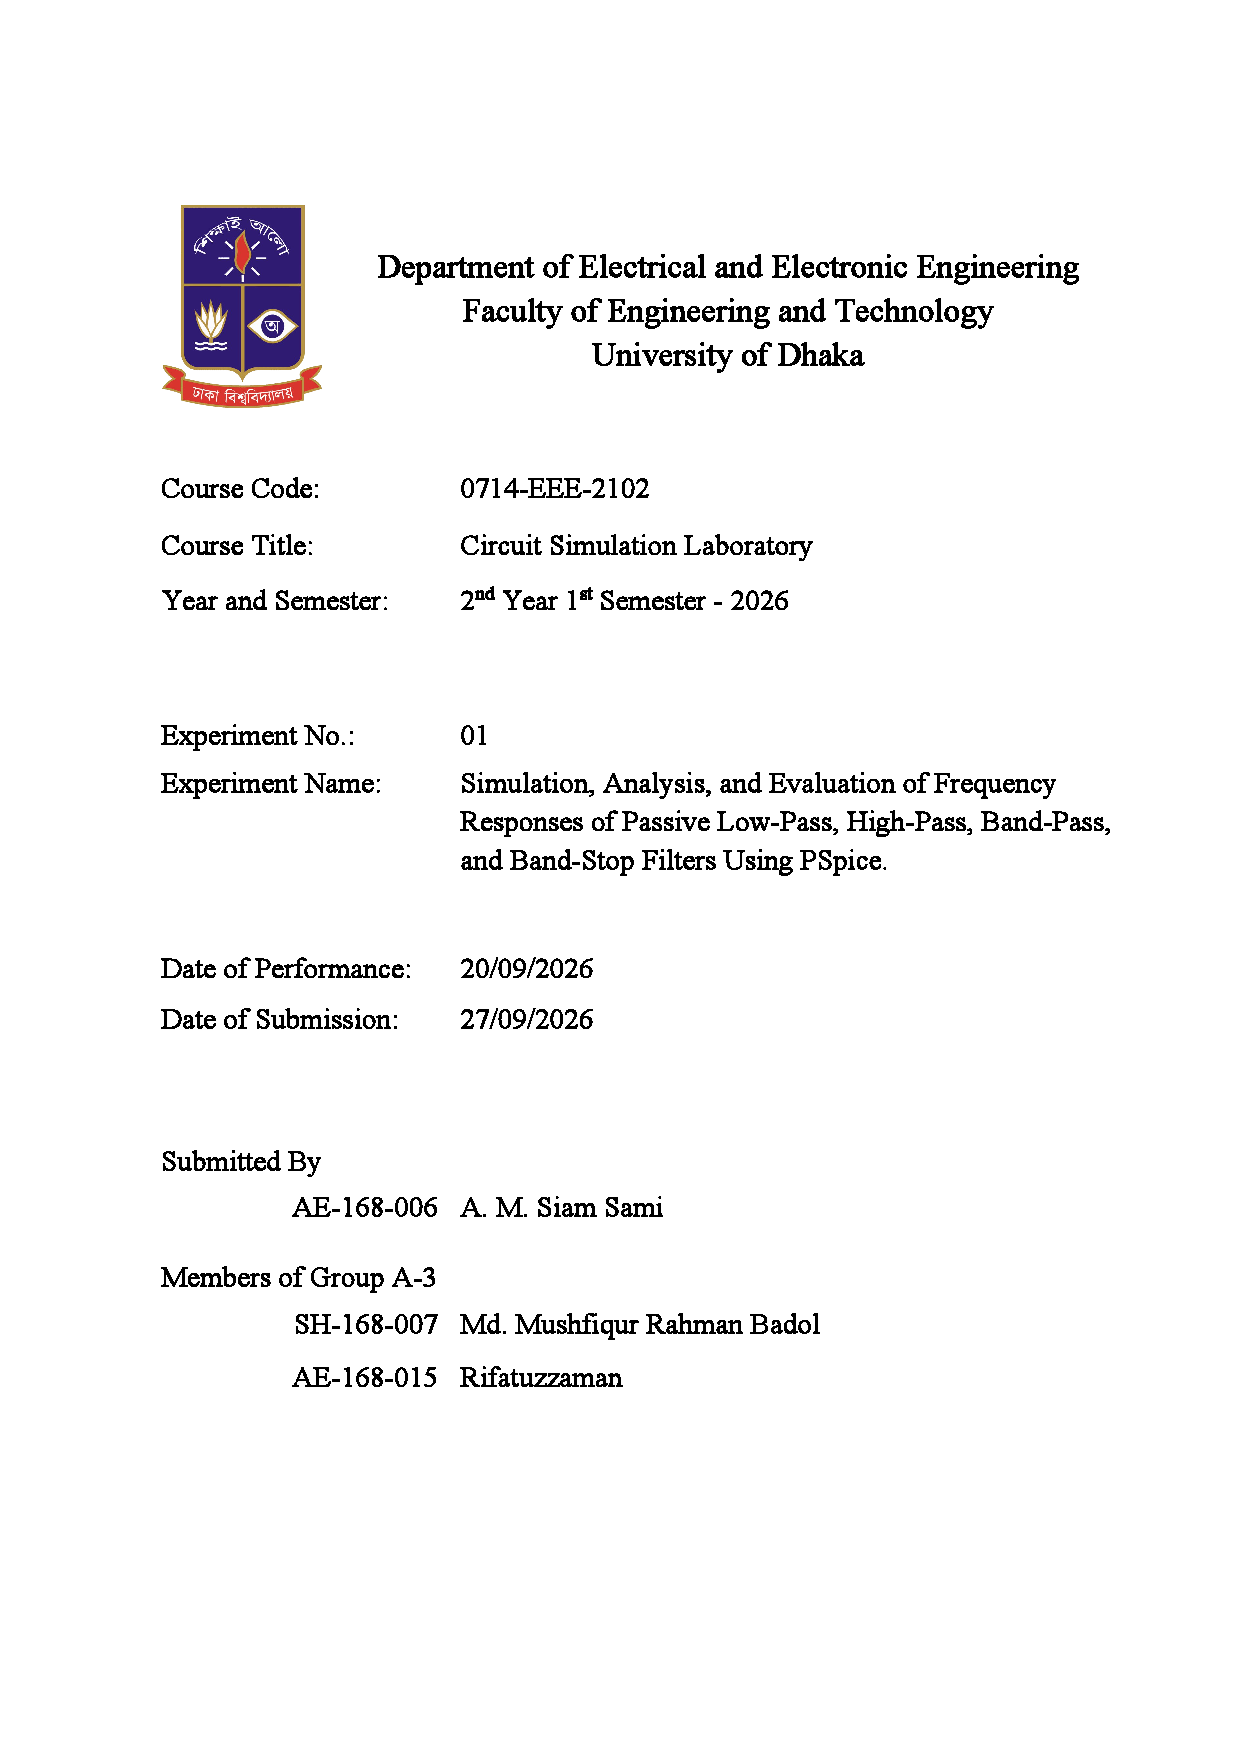
\includepdf[pages={1}]{../Cover_page.pdf}
	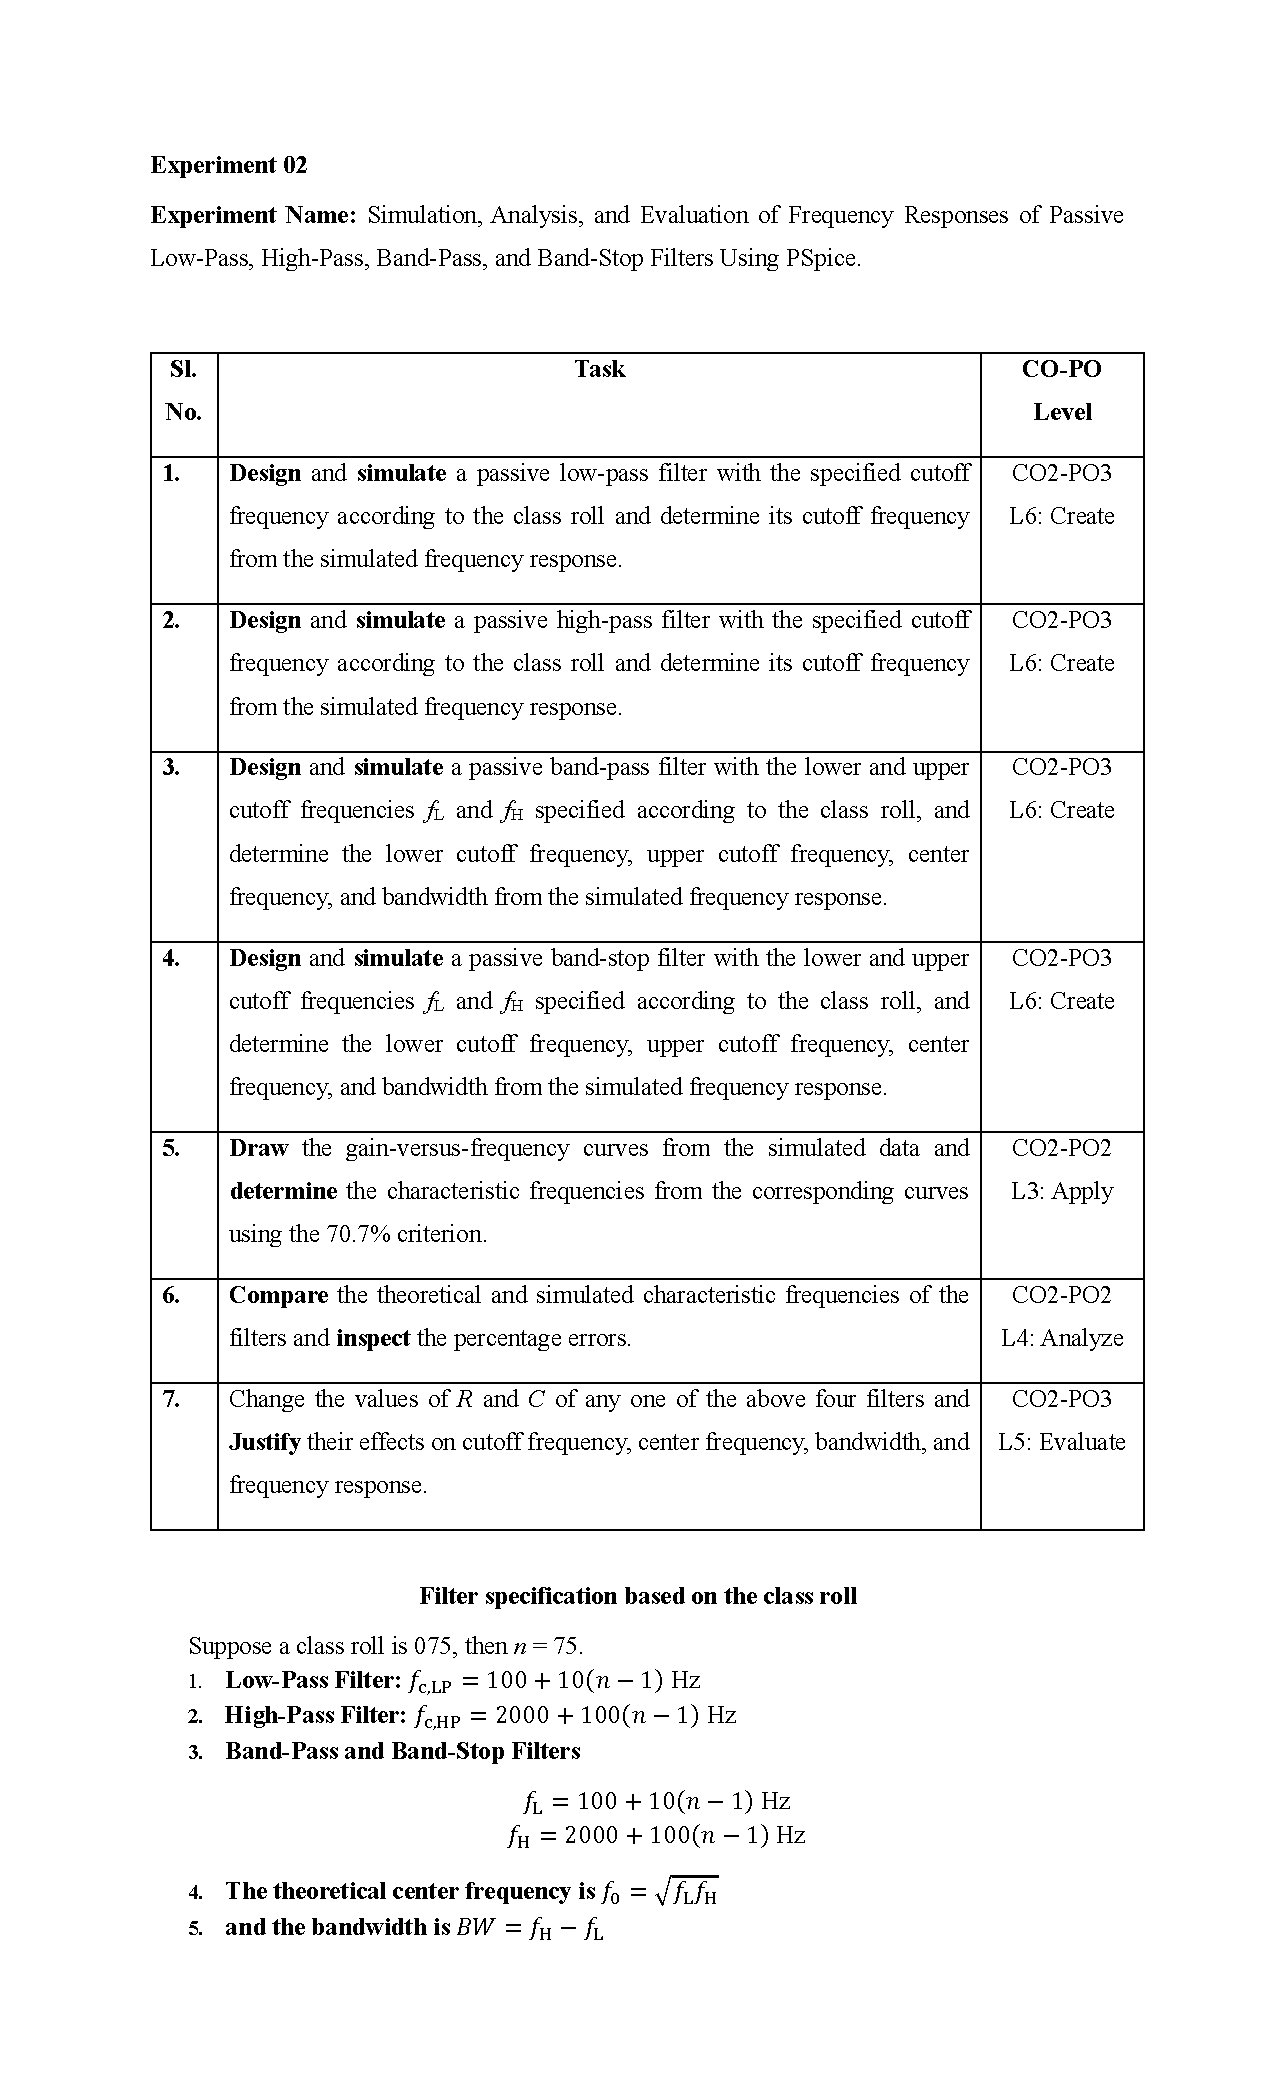
\includepdf[pages={1}]{../2nd_page.pdf}
	\includepdf[pages={2}]{../2nd_page.pdf}
	
	% =====================================================================
	% HEADER BLOCK
	% =====================================================================
	\begin{center}
		{\large\bfseries Experiment No. \expnumber}\\[4pt]
		{\large\bfseries Name of the Experiment: Simulation, Analysis, and
			Evaluation of Frequency Responses of Passive Low-Pass, High-Pass,
			Band-Pass, and Band-Stop Filters Using PSpice}
	\end{center}
	\vspace{6pt}
	
	% =====================================================================
	\section{Objective}
	% =====================================================================
	The purposes of this experiment are-
	\begin{enumerate}[label=\arabic*.]
		\item Designing of a low-pass circuit to pass the desired low frequency signals and stop the unwanted high frequency signals.
		\item Designing of a high-pass circuit to pass the desired high frequency signals and stop the unwanted low frequency signals.
		\item Designing of a band-pass circuit that allows signals between two specific frequencies to pass and discriminates against signals at other frequencies.
		\item Designing of a stop-band circuit that rejects a band of frequencies and let through signals at other frequencies.
		\item Verifying the frequency responses of the above low-pass, high-pass, band-pass and stop-band filters.
	\end{enumerate}
	\section{Theory}
	
	A frequency-selective circuit changes the amplitude and phase of a sinusoidal signal according to frequency. For a linear circuit, its frequency response is represented by the transfer function
	\begin{equation}
		H(j\omega)=\frac{V_{\mathrm{out}}(j\omega)}{V_{\mathrm{in}}(j\omega)},
		\qquad \omega=2\pi f .
		\label{eq:transfer-general}
	\end{equation}
	The voltage gain may be expressed either as the magnitude $|H(j\omega)|$ or in decibels as
	\begin{equation}
		G_{\mathrm{dB}}=20\log_{10}|H(j\omega)| .
		\label{eq:gain-db}
	\end{equation}
	At a cutoff frequency, the output magnitude is $1/\sqrt{2}=0.707$ of the corresponding passband value, and therefore
	\begin{equation}
		20\log_{10}\left(\frac{1}{\sqrt{2}}\right)\approx-3.01\,\mathrm{dB}.
		\label{eq:cutoff-db}
	\end{equation}
	Thus, the 70.7\% voltage criterion and the $-3\,\mathrm{dB}$ criterion identify the same cutoff point \cite{ref:sadiku}\cite{ref:boylestad}.
	
	\subsection*{Low-Pass Filter}
	
	A first-order passive RC low-pass filter passes low-frequency signals and attenuates signals above its cutoff frequency. In Fig.~\ref{fig:lp-theory}, the output is measured across the capacitor. Since the capacitor impedance is
	\begin{equation}
		Z_C=\frac{1}{j\omega C},
		\label{eq:zc}
	\end{equation}
	voltage division gives
	\begin{equation}
		H_{\mathrm{LP}}(j\omega)
		=\frac{V_{\mathrm{out}}}{V_{\mathrm{in}}}
		=\frac{Z_C}{R+Z_C}
		=\frac{1}{1+j\omega RC}.
		\label{eq:lp-transfer}
	\end{equation}
	
	\begin{figure}[htbp]
		\centering
		\begin{circuitikz}[american voltages]
			\draw (0,0) to[sV,l_=$V_{\mathrm{in}}$] (0,2)
			to[R,l=$R$] (3,2) coordinate (out)
			to[C,l=$C$] (3,0) -- (0,0);
			\draw (1.5,0) node[ground]{};
			\draw (out) -- (4,2) node[ocirc,label=right:$V_{\mathrm{out}}$]{};
		\end{circuitikz}
		\caption{First-order passive RC low-pass filter.}
		\label{fig:lp-theory}
	\end{figure}
	
	The magnitude response is
	\begin{equation}
		|H_{\mathrm{LP}}(j\omega)|
		=\frac{1}{\sqrt{1+(\omega RC)^2}}.
		\label{eq:lp-magnitude}
	\end{equation}
	At cutoff, $|H_{\mathrm{LP}}(j\omega_c)|=1/\sqrt{2}$. Hence,
	\begin{equation}
		\frac{1}{\sqrt{1+(2\pi f_cRC)^2}}=\frac{1}{\sqrt{2}},
		\label{eq:lp-cutoff-condition}
	\end{equation}
	which reduces to
	\begin{equation}
		2\pi f_cRC=1.
		\label{eq:lp-cutoff-step}
	\end{equation}
	Therefore, the cutoff frequency is
	\begin{equation}
		f_c=\frac{1}{2\pi RC}.
		\label{eq:lp-cutoff}
	\end{equation}
	Below $f_c$, the output approaches the input magnitude; above $f_c$, the magnitude decreases at approximately $20\,\mathrm{dB/decade}$ \cite{ref:sadiku}\cite{ref:boylestad}.
	
	\subsection{High-Pass Filter}
	
	A first-order passive RC high-pass filter attenuates low-frequency signals and passes signals above its cutoff frequency. The output in Fig.~\ref{fig:hp-theory} is measured across the resistor. Voltage division gives
	\begin{equation}
		H_{\mathrm{HP}}(j\omega)
		=\frac{V_{\mathrm{out}}}{V_{\mathrm{in}}}
		=\frac{R}{R+Z_C}
		=\frac{j\omega RC}{1+j\omega RC}.
		\label{eq:hp-transfer}
	\end{equation}
	
	\begin{figure}[htbp]
		\centering
		\begin{circuitikz}[american voltages]
			\draw (0,0) to[sV,l_=$V_{\mathrm{in}}$] (0,2)
			to[C,l=$C$] (3,2) coordinate (out)
			to[R,l=$R$] (3,0) -- (0,0);
			\draw (1.5,0) node[ground]{};
			\draw (out) -- (4,2) node[ocirc,label=right:$V_{\mathrm{out}}$]{};
		\end{circuitikz}
		\caption{First-order passive RC high-pass filter.}
		\label{fig:hp-theory}
	\end{figure}
	
	Its magnitude response is
	\begin{equation}
		|H_{\mathrm{HP}}(j\omega)|
		=\frac{\omega RC}{\sqrt{1+(\omega RC)^2}}.
		\label{eq:hp-magnitude}
	\end{equation}
	Applying the cutoff condition gives
	\begin{equation}
		\frac{2\pi f_cRC}{\sqrt{1+(2\pi f_cRC)^2}}
		=\frac{1}{\sqrt{2}},
		\label{eq:hp-cutoff-condition}
	\end{equation}
	and hence
	\begin{equation}
		f_c=\frac{1}{2\pi RC}.
		\label{eq:hp-cutoff}
	\end{equation}
	Below $f_c$, the gain rises at approximately $20\,\mathrm{dB/decade}$; sufficiently above $f_c$, it approaches unity \cite{ref:sadiku}\cite{ref:boylestad}.
	
	\subsection{Band-Pass Filter}
	
	A series-resonant RLC circuit acts as a band-pass filter when the output is measured across the resistor, as shown in Fig.~\ref{fig:bp-theory}. At very low frequencies the capacitor reactance is large, while at very high frequencies the inductor reactance is large; in both cases the circuit current and the resistor voltage are small. Near resonance, the inductive and capacitive reactances cancel, the current is maximum, and the output across $R$ reaches its maximum value \cite{ref:sadiku}\cite{ref:boylestad}.
	
	\begin{figure}[htbp]
		\centering
		\begin{circuitikz}[american voltages]
			\draw (0,0) to[sV,l_=$V_{\mathrm{in}}$] (0,3)
			to[L,l=$L$] (2,3)
			to[C,l=$C$] (4,3) coordinate (out)
			to[R,l=$R$] (4,0) -- (0,0);
			\draw (2,0) node[ground]{};
			\draw (out) -- (5.1,3) node[ocirc,label=right:$V_{\mathrm{out}}$]{};
		\end{circuitikz}
		\caption{Series RLC band-pass filter with the output measured across $R$.}
		\label{fig:bp-theory}
	\end{figure}
	
	The total series impedance is
	\begin{equation}
		Z=R+j\left(\omega L-\frac{1}{\omega C}\right).
		\label{eq:rlc-total-z}
	\end{equation}
	Therefore, the band-pass transfer function is
	\begin{equation}
		H_{\mathrm{BP}}(j\omega)
		=\frac{V_{\mathrm{out}}}{V_{\mathrm{in}}}
		=\frac{R}{R+j\left(\omega L-\dfrac{1}{\omega C}\right)}.
		\label{eq:bp-transfer}
	\end{equation}
	Its magnitude is
	\begin{equation}
		|H_{\mathrm{BP}}(j\omega)|
		=\frac{R}{\sqrt{R^2+\left(\omega L-\dfrac{1}{\omega C}\right)^2}}.
		\label{eq:bp-magnitude}
	\end{equation}
	At resonance, the inductive and capacitive reactances cancel:
	\begin{equation}
		\omega_0L=\frac{1}{\omega_0C}.
		\label{eq:resonance-condition}
	\end{equation}
	Thus, the center frequency is
	\begin{equation}
		f_0=\frac{1}{2\pi\sqrt{LC}}=\sqrt{f_Lf_H}.
		\label{eq:rlc-f0}
	\end{equation}
	At either half-power cutoff frequency, $|H_{\mathrm{BP}}|=1/\sqrt{2}$, which gives
	\begin{equation}
		\left|\omega L-\frac{1}{\omega C}\right|=R.
		\label{eq:rlc-cutoff-condition}
	\end{equation}
	Solving the lower- and upper-cutoff equations gives
	\begin{equation}
		\omega_H-\omega_L=\frac{R}{L}.
		\label{eq:rlc-angular-bw}
	\end{equation}
	Hence, the bandwidth and quality factor are
	\begin{equation}
		BW=f_H-f_L=\frac{R}{2\pi L}
		\label{eq:rlc-bw}
	\end{equation}
	and
	\begin{equation}
		Q=\frac{f_0}{BW}=\frac{1}{R}\sqrt{\frac{L}{C}},
		\label{eq:rlc-q}
	\end{equation}
	respectively. The cutoff frequencies also satisfy
	\begin{equation}
		f_Lf_H=f_0^2.
		\label{eq:rlc-cutoff-product}
	\end{equation}
	The frequency interval $f_L<f<f_H$ is the passband, and the ideal gain at resonance is unity.
	
	\subsection{Band-Stop Filter}
	
	A band-stop, or notch, filter passes frequencies below and above a rejected band. Figure~\ref{fig:bs-theory} shows a series RLC notch network in which the output is measured across the series $LC$ branch. This output location is essential: measuring across $R$ would instead produce a band-pass response.
	
	\begin{figure}[htbp]
		\centering
		\begin{circuitikz}[american voltages]
			\draw (0,0) to[sV,l_=$V_{\mathrm{in}}$] (0,3)
			to[R,l=$R$] (3,3) coordinate (out)
			to[C,l=$C$] (3,1.5)
			to[L,l=$L$] (3,0) -- (0,0);
			\draw (1.5,0) node[ground]{};
			\draw (out) -- (4.3,3) node[ocirc,label=right:$V_{\mathrm{out}}$]{};
		\end{circuitikz}
		\caption{Series RLC band-stop filter with the output measured across the series $LC$ branch.}
		\label{fig:bs-theory}
	\end{figure}
	
	The series-network impedance is given by Eq.~\eqref{eq:rlc-total-z}, while the impedance of the output branch is
	\begin{equation}
		Z_{LC}=j\left(\omega L-\frac{1}{\omega C}\right),
		\label{eq:lc-z}
	\end{equation}
	Therefore,
	\begin{equation}
		H_{\mathrm{BS}}(j\omega)
		=\frac{Z_{LC}}{R+Z_{LC}}
		=\frac{j\left(\omega L-\dfrac{1}{\omega C}\right)}
		{R+j\left(\omega L-\dfrac{1}{\omega C}\right)}.
		\label{eq:bs-transfer}
	\end{equation}
	Its magnitude is
	\begin{equation}
		|H_{\mathrm{BS}}(j\omega)|
		=\frac{\left|\omega L-\dfrac{1}{\omega C}\right|}
		{\sqrt{R^2+\left(\omega L-\dfrac{1}{\omega C}\right)^2}}.
		\label{eq:bs-magnitude}
	\end{equation}
	At the resonance condition of Eq.~\eqref{eq:resonance-condition}, $Z_{LC}=0$ and the ideal output becomes zero. The notch center frequency is given by Eq.~\eqref{eq:rlc-f0}.
	At either cutoff, $|H_{\mathrm{BS}}|=1/\sqrt{2}$, which requires
	\begin{equation}
		\left|\omega L-\frac{1}{\omega C}\right|=R.
		\label{eq:bs-cutoff-condition}
	\end{equation}
	Consequently, the band-stop filter has the same center-frequency, cutoff-frequency, bandwidth, and quality-factor relationships as Eqs.~\eqref{eq:rlc-f0}--\eqref{eq:rlc-cutoff-product}; however, its magnitude response is complementary to that of the resistor-output band-pass circuit. Practical inductors introduce winding resistance and parasitic effects that reduce the notch depth \cite{ref:sadiku}\cite{ref:boylestad}.
	
	\subsection{Comparison with Simulation}
	
	The characteristic frequencies obtained from the simulated gain curves will be compared with the theoretical values by the absolute percentage error
	\begin{equation}
		\%\,\mathrm{Error}
		=\left|\frac{\text{Theoretical value}-\text{Simulated value}}
		{\text{Theoretical value}}\right|\times100.
		\label{eq:percentage-error}
	\end{equation}
	The analysis assumes ideal lumped components and an ideal source with zero internal resistance. Component tolerances, source and measurement loading, inductor winding resistance and parasitic effects, and the finite frequency resolution of the AC sweep can cause deviations between calculated and simulated characteristic frequencies.
	
	
	% =====================================================================
	\section{Design}
	% =====================================================================
	The class roll number is $n = 6$, so the specified (formula) cutoff
	frequencies are
	\begin{itemize}
		\item Low-pass filter:
		$f_{c,\mathrm{LP}} = 100 + 10(n-1) = 100 + 10\cdot 5
		= \SI{150}{\hertz}$.
		\item High-pass filter:
		$f_{c,\mathrm{HP}} = 2000 + 100(n-1) = 2000 + 100\cdot 5
		= \SI{2500}{\hertz}$.
		\item Band-pass and band-stop filters:
		$f_{L} = \SI{150}{\hertz}$, $f_{H} = \SI{2500}{\hertz}$, with
		$f_{0} = \sqrt{f_{L}f_{H}} = \sqrt{150\cdot 2500}
		= \SI{612.4}{\hertz}$ and
		$BW = f_{H}-f_{L} = \SI{2350}{\hertz}$.
	\end{itemize}
	
	Component values were then selected from the standard E-series so that
	the formula frequencies are reproduced as closely as possible; the
	actual frequencies produced by the chosen standard values are the
	\textbf{theoretical values} against which the simulation is compared.
	
	\subsection{Low-pass filter (circuit 1)}
	Choosing the standard capacitor $C = \SI{100}{\nano\farad}$,
	\eqref{eq:lp-cutoff} requires
	\[
	R = \frac{1}{2\pi f_{c} C}
	= \frac{1}{2\pi \cdot 150 \cdot 100\times 10^{-9}}
	= \SI{10.61}{\kilo\ohm},
	\]
	so the nearest standard value $R = \SI{10.7}{\kilo\ohm}$ was used.
	
	\subsection{High-pass filter (circuit 2)}
	Choosing the standard capacitor $C = \SI{10}{\nano\farad}$,
	\[
	R = \frac{1}{2\pi f_{c} C}
	= \frac{1}{2\pi \cdot 2500 \cdot 10\times 10^{-9}}
	= \SI{6.37}{\kilo\ohm},
	\]
	and the nearest standard value $R = \SI{6.34}{\kilo\ohm}$ was used.
	
	\subsection{Band-pass and band-stop filters (circuits 3 and 4)}
	Both use the same series RLC loop with a standard
	$C = \SI{10}{\micro\farad}$. From \eqref{eq:rlc-f0}, the inductor needed
	for $f_0 = \SI{612.4}{\hertz}$ is
	\[
	L = \frac{1}{(2\pi f_{0})^{2} C}
	= \frac{1}{(2\pi \cdot 612.4)^{2} \cdot 10\times 10^{-6}}
	= \SI{6.75}{\milli\henry},
	\]
	rounded to the standard value $L = \SI{6.8}{\milli\henry}$. From
	\eqref{eq:rlc-bw}, the resistance setting $BW = \SI{2350}{\hertz}$ is
	\[
	R = 2\pi L \cdot BW = 2\pi \cdot 6.8\times 10^{-3} \cdot 2350
	= \SI{100.4}{\ohm},
	\]
	rounded to the standard value $R = \SI{100}{\ohm}$. The band-pass
	circuit takes the output across $R$; the band-stop circuit takes it
	across the series $LC$ pair.
	
	\subsection{Modified low-pass filter (task 7)}
	The resistor and capacitor of circuit 1 were changed to the standard
	values $R = \SI{2.2}{\kilo\ohm}$ and $C = \SI{1}{\micro\farad}$ to
	evaluate the effect of $R$ and $C$ on the response.
	
	% =====================================================================
	\section{List of Components}
	% =====================================================================
	\begin{table}[H]
		\centering
		\caption{Components, instruments, and software used}
		\label{tab:components}
		\renewcommand{\arraystretch}{1.25}
		\begin{tabular}{|c|l|l|S|}
			\hline
			\rowcolor{black!12}\textbf{Sl. No.} & \textbf{Component/Instrument} & \textbf{Specification/Value} & {\textbf{Quantity}} \\
			\hline
			1 & Resistor & \SI{10.7}{\kilo\ohm} (circuit 1) & 1 \\
			\hline
			2 & Resistor & \SI{6.34}{\kilo\ohm} (circuit 2) & 1 \\
			\hline
			3 & Resistor & \SI{100}{\ohm} (circuits 3--4)   & 2 \\
			\hline
			4 & Resistor & \SI{2.2}{\kilo\ohm} (circuit 1, modified) & 1 \\
			\hline
			5 & Capacitor & \SI{100}{\nano\farad} (circuit 1) & 1 \\
			\hline
			6 & Capacitor & \SI{10}{\nano\farad} (circuit 2)  & 1 \\
			\hline
			7 & Capacitor & \SI{10}{\micro\farad} (circuits 3--4) & 2 \\
			\hline
			8 & Capacitor & \SI{1}{\micro\farad} (circuit 1, modified) & 1 \\
			\hline
			9 & Inductor & \SI{6.8}{\milli\henry} (circuits 3--4) & 2 \\
			\hline
			10 & AC voltage source & VAC, magnitude \SI{5}{\volt}, phase \SI{0}{\degree} & 5 \\
			\hline
			11 & Simulation software & PSpice & 1 \\
			\hline
			12 & Plotting software & OriginPro & 1 \\
			\hline
		\end{tabular}
	\end{table}
	
	\section{PSpice Circuit Diagrams}
	% The actual PSpice schematic exports.
	% =====================================================================
	\begin{figure}[H]
		\centering
		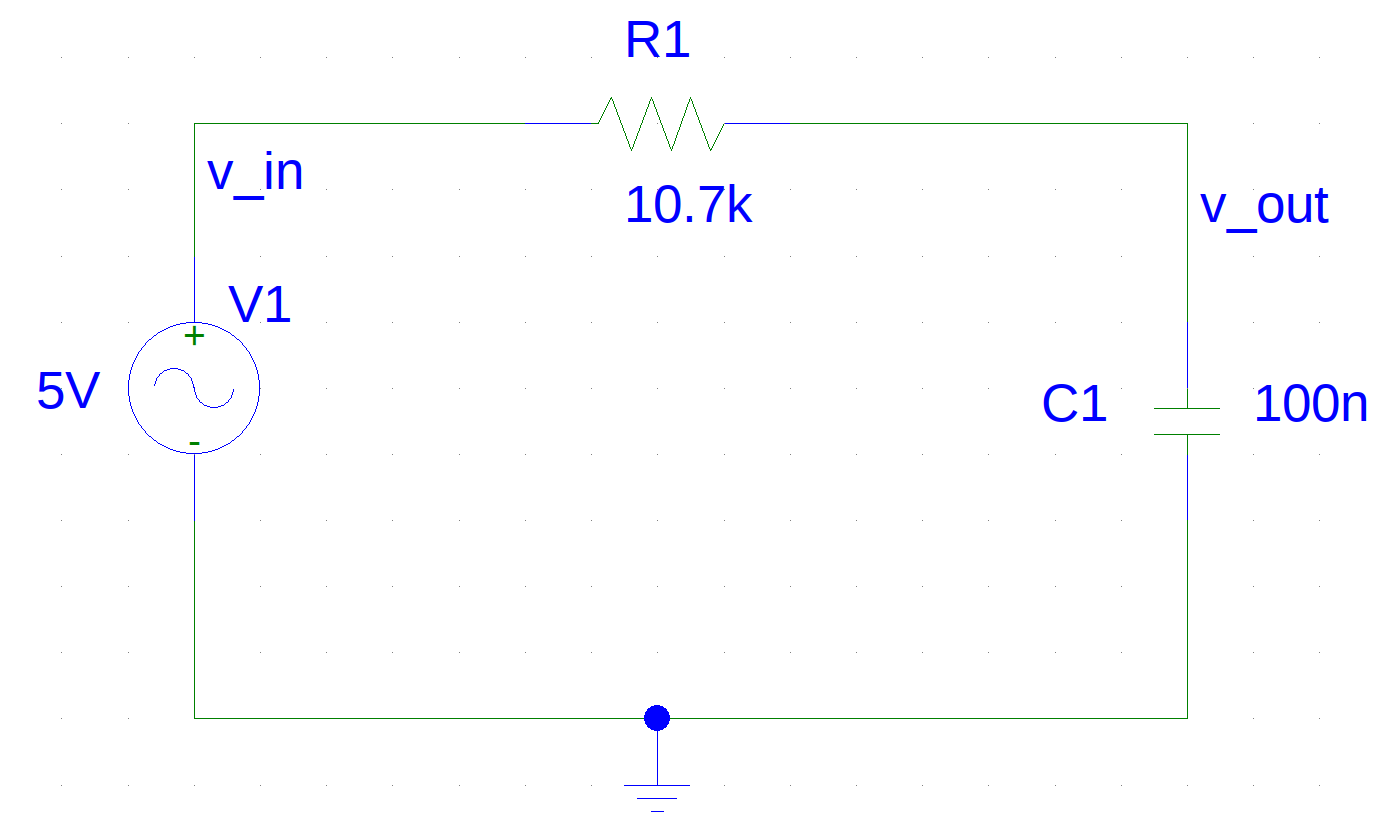
\includegraphics[width=0.9\textwidth]{circuit1.png}
		\caption{PSpice schematic of circuit 1: passive low-pass RC filter
			($R = \SI{10.7}{\kilo\ohm}$, $C = \SI{100}{\nano\farad}$),
			output taken across the capacitor}
		\label{fig:sch1}
	\end{figure}
	
	\begin{figure}[H]
		\centering
		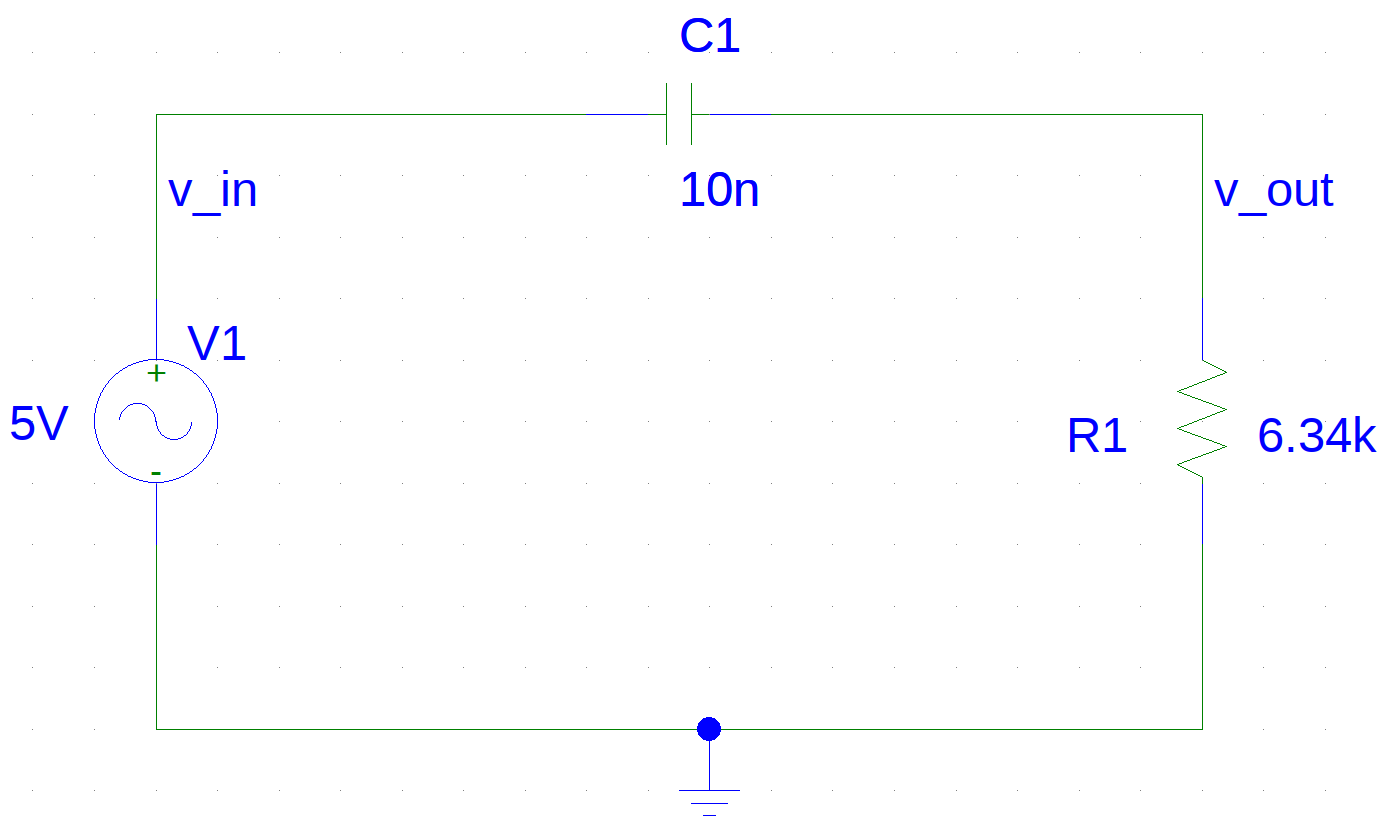
\includegraphics[width=0.9\textwidth]{circuit2.png}
		\caption{PSpice schematic of circuit 2: passive high-pass RC filter
			($R = \SI{6.34}{\kilo\ohm}$, $C = \SI{10}{\nano\farad}$),
			output taken across the resistor}
		\label{fig:sch2}
	\end{figure}
	
	\begin{figure}[H]
		\centering
		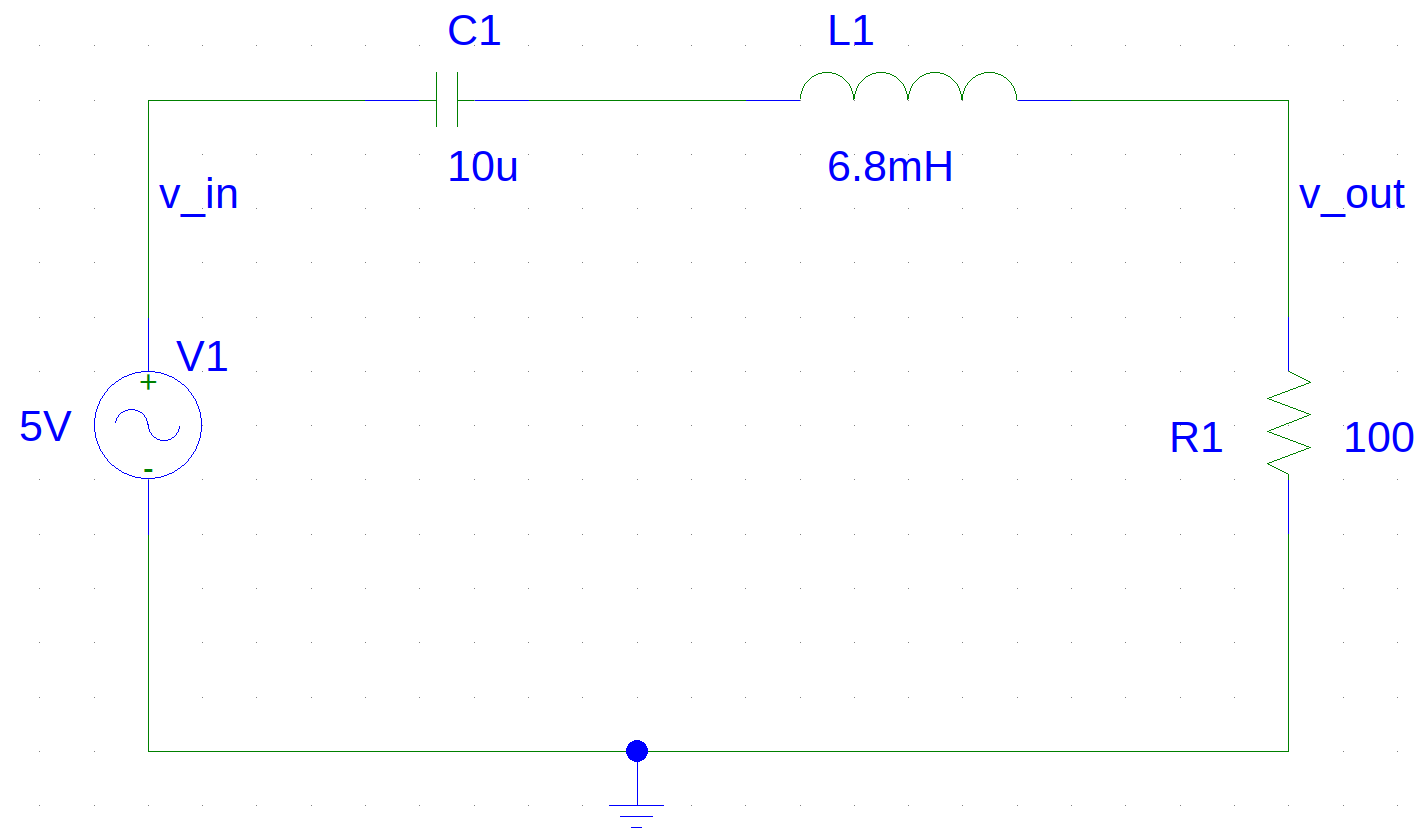
\includegraphics[width=0.9\textwidth]{circuit3.png}
		\caption{PSpice schematic of circuit 3: passive band-pass series RLC
			filter ($R = \SI{100}{\ohm}$, $L = \SI{6.8}{\milli\henry}$,
			$C = \SI{10}{\micro\farad}$), output taken across the
			resistor}
		\label{fig:sch3}
	\end{figure}
	
	\begin{figure}[H]
		\centering
		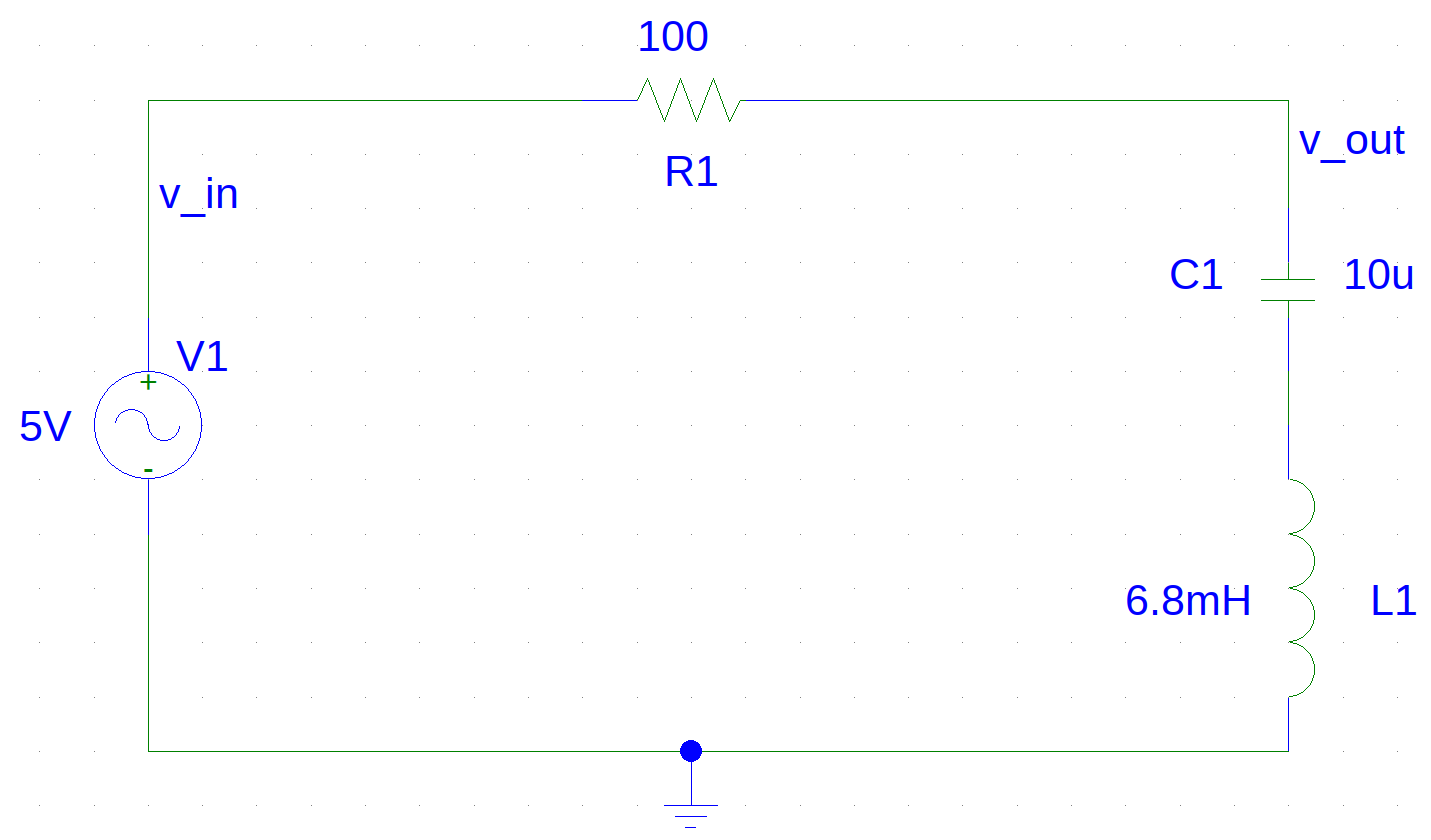
\includegraphics[width=0.9\textwidth]{circuit4.png}
		\caption{PSpice schematic of circuit 4: passive band-stop series RLC
			filter ($R = \SI{100}{\ohm}$, $L = \SI{6.8}{\milli\henry}$,
			$C = \SI{10}{\micro\farad}$), output taken across the series
			$LC$ pair}
		\label{fig:sch4}
	\end{figure}
	
	\begin{figure}[H]
		\centering
		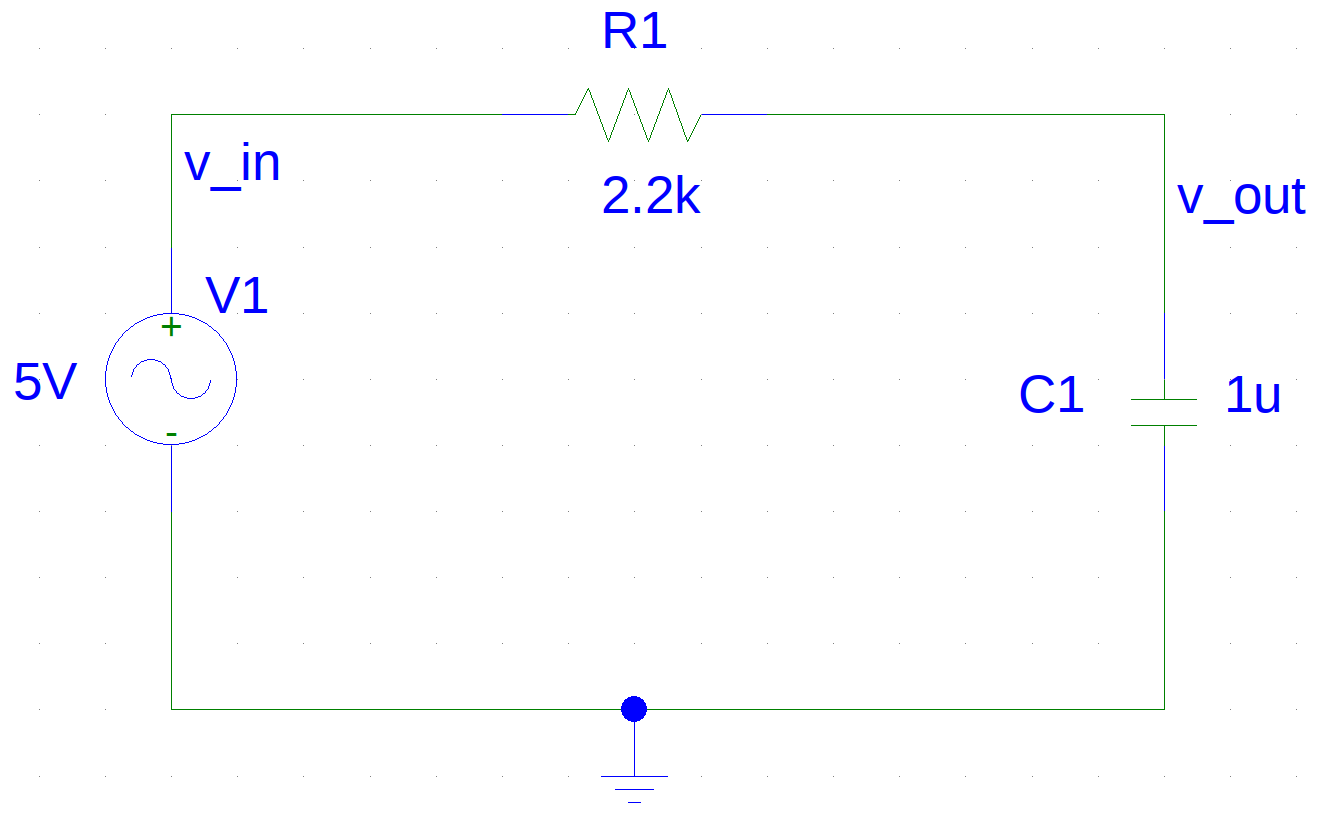
\includegraphics[width=0.9\textwidth]{circuit1_changed.png}
		\caption{PSpice schematic of the modified low-pass filter of task 7
			(circuit 1 with $R = \SI{2.2}{\kilo\ohm}$,
			$C = \SI{1}{\micro\farad}$)}
		\label{fig:sch1c}
	\end{figure}
	
	% =====================================================================
	
	% =====================================================================
	\section{Simulation/Working Procedure}
	
	PSpice 9.1 Schematics was used to construct the circuits and perform AC-sweep simulations. OriginPro 2018 was used to tabulate the simulated data, plot the final gain-versus-frequency curves, determine the characteristic frequencies, and calculate percentage errors. The procedure was divided into the following two parts.
	
	\subsection*{Part 1: Simulation in PSpice 9.1 Schematics}
	
	\begin{enumerate}[leftmargin=0.8cm,label=\textbf{Step \arabic*:},itemsep=0.55em]
		\item \textbf{Draw the schematics.}
		Open PSpice 9.1 Schematics. Select \texttt{Draw $\rightarrow$ Get New Part} or press \texttt{Ctrl+G}. Place the required resistors, capacitors, inductors, AC voltage source (VAC), and analog ground (AGND/EGND) on the workspace. Construct the low-pass, high-pass, series RLC band-pass, and series RLC band-stop circuits according to Figs.~\ref{fig:sch1}--\ref{fig:sch1c}.
		
		Double-click each component and assign the values calculated in Section 1.3. For example, use $R=10.7\,\mathrm{k}\Omega$ and $C=100\,\mathrm{n}\mathrm{F}$ for the low-pass filter. Set the AC magnitude of the VAC source to $5\,\mathrm{V}$. Use \texttt{Draw $\rightarrow$ Wire}, or press \texttt{Ctrl+W}, to connect the circuit. Label the source and output nodes as \texttt{Vin} and \texttt{Vout}, respectively, and verify that each circuit has one analog-ground reference.
		
		\item \textbf{Set up the AC sweep.}
		Select \texttt{Analysis $\rightarrow$ Setup}, enable \texttt{AC Sweep}, and open its settings. Select a decade sweep and enter the following parameters:
		\begin{center}
			\begin{tabular}{@{}ll@{}}
				Points per decade: & 100 \\
				Start frequency: & $1\,\mathrm{Hz}$ \\
				End frequency: & $100\,\mathrm{kHz}$
			\end{tabular}
		\end{center}
		Click \texttt{OK}, close the setup window, and save the schematic with an identifiable name, such as \texttt{LowPassFilter.sch}.
		
		\item \textbf{Run the simulation and display the gain.}
		Select \texttt{Analysis $\rightarrow$ Simulate}, or press \texttt{F11}. When the Probe window opens, select \texttt{Trace $\rightarrow$ Add Trace}. Enter
		\begin{equation}
			\texttt{DB(V(Vout)/V(Vin))}
			\label{eq:pspice-db-trace}
		\end{equation}
		in the trace-expression box to display the voltage gain in decibels. Confirm that the plotted response has the expected low-pass, high-pass, band-pass, or band-stop shape.
		
		\item \textbf{Measure and record the output voltage.}
		Delete the decibel trace and add \texttt{V(Vout)} to display the output-voltage amplitude. Enable the cursor from \texttt{Trace $\rightarrow$ Cursor $\rightarrow$ Display}. Move the cursor along the frequency axis and record $V_{\mathrm{out}}$ at each frequency specified in the experimental data tables. Record enough points near each cutoff frequency and, for the RLC filters, near the resonant frequency to define the curve accurately.
		
		\item \textbf{Repeat for all filters.}
		Repeat Steps 1--4 for the high-pass, band-pass, and band-stop filters. For the band-pass filter, measure the output across $R$. For the band-stop filter, measure the output across the series $LC$ combination. Export or manually tabulate the frequency and output-voltage data for processing in OriginPro.
	\end{enumerate}
	
	\subsection*{Part 2: Plotting and Analysis in OriginPro 2018}
	
	\begin{enumerate}[leftmargin=0.8cm,label=\textbf{Step \arabic*:},itemsep=0.55em]
		\item \textbf{Enter the simulation data.}
		Launch OriginPro 2018 and prepare a separate worksheet for each filter. Assign the worksheet columns as follows:
		\begin{center}
			\begin{tabular}{@{}ll@{}}
				Column A (X): & Input frequency, $f$ ($\mathrm{Hz}$) \\
				Column B (Y): & Simulated output voltage, $V_{\mathrm{out}}$ ($\mathrm{V}$) \\
				Column C (Y): & Voltage gain, $A_v=V_{\mathrm{out}}/V_{\mathrm{in}}$
			\end{tabular}
		\end{center}
		If a decibel plot is required, calculate the gain using Eq.~\eqref{eq:gain-db}. Enter the recorded PSpice data in the corresponding rows.
		
		\item \textbf{Plot the frequency response.}
		Highlight the frequency column and the gain or output-voltage column. Select \texttt{Plot $\rightarrow$ Line + Symbol} or \texttt{Scatter} to create the discrete-point graph. Connect the points with a smooth curve without altering the recorded data. Double-click the horizontal axis, open the \texttt{Scale} tab, and select \texttt{Logarithmic (Log10)} so that the complete frequency range is displayed clearly.
		
		\item \textbf{Determine the cutoff frequencies by the 70.7\% criterion.}
		Determine the appropriate passband or peak output voltage $V_{\max}$ from the plotted curve. The cutoff-reference voltage is
		\begin{equation}
			V_{\mathrm{cutoff}}=0.707V_{\max}.
			\label{eq:cutoff-reference-voltage}
		\end{equation}
		Use the \texttt{Screen Reader} or \texttt{Data Reader} tool to locate the intersection of the response curve with $V_{\mathrm{cutoff}}$. The corresponding frequency is the simulated cutoff frequency. For both band-pass and band-stop filters, locate the lower and upper intersections, $f_L$ and $f_H$, and calculate
		\begin{equation}
			BW_{\mathrm{sim}}=f_{H,\mathrm{sim}}-f_{L,\mathrm{sim}}
			\label{eq:simulated-bandwidth}
		\end{equation}
		and
		\begin{equation}
			f_{0,\mathrm{sim}}=\sqrt{f_{L,\mathrm{sim}}f_{H,\mathrm{sim}}}.
			\label{eq:simulated-center-frequency}
		\end{equation}
		Use interpolation between adjacent data points when an exact 70.7\% crossing is not directly available.
		
		\item \textbf{Calculate percentage errors.}
		Compare each simulated cutoff frequency, center frequency, and bandwidth with its corresponding theoretical value. Use Eq.~\eqref{eq:percentage-error} through an Origin column formula or by direct calculation. Record the theoretical value, simulated value, absolute difference, and percentage error in the result tables.
	\end{enumerate}
	
	\section{Result Analysis}
	% =====================================================================
	\subsection{Theoretical characteristic frequencies (standard values)}
	The standard component values do not reproduce the formula frequencies
	exactly; substituting them into the derived equations gives the
	theoretical values.
	
	\textbf{Low-pass filter:} from \eqref{eq:lp-cutoff}, with
	$R = \SI{10.7}{\kilo\ohm}$, $C = \SI{100}{\nano\farad}$:
	\begin{equation}
		f_{c} = \frac{1}{2\pi RC}
		= \frac{1}{2\pi \cdot 10.7\times 10^{3} \cdot 100\times 10^{-9}}
		= \SI{148.7}{\hertz}.
		\label{eq:calc-lp}
	\end{equation}
	
	\textbf{High-pass filter:} with $R = \SI{6.34}{\kilo\ohm}$,
	$C = \SI{10}{\nano\farad}$:
	\begin{equation}
		f_{c} = \frac{1}{2\pi \cdot 6.34\times 10^{3} \cdot 10\times 10^{-9}}
		= \SI{2510.3}{\hertz}.
		\label{eq:calc-hp}
	\end{equation}
	
	\textbf{Band-pass and band-stop filters:} with $R = \SI{100}{\ohm}$,
	$L = \SI{6.8}{\milli\henry}$, $C = \SI{10}{\micro\farad}$.
	From \eqref{eq:rlc-f0}:
	\begin{equation}
		f_{0} = \frac{1}{2\pi\sqrt{6.8\times 10^{-3}\cdot 10\times 10^{-6}}}
		= \frac{1}{2\pi\sqrt{6.8\times 10^{-8}}}
		= \SI{610.3}{\hertz}.
		\label{eq:calc-f0}
	\end{equation}
	From \eqref{eq:rlc-cutoff-condition}, using
	$R/2L = 7352.9\ \mathrm{rad/s}$ and
	\[
	\sqrt{(R/2L)^{2} + \frac{1}{LC}}
	= \sqrt{7352.9^{2} + 1.4706\times 10^{7}}
	= 8292.8\ \mathrm{rad/s}:
	\]
	\begin{align}
		f_{H} &= \frac{7352.9 + 8292.8}{2\pi} = \SI{2490.1}{\hertz},
		\label{eq:calc-fH}\\
		f_{L} &= \frac{8292.8 - 7352.9}{2\pi} = \SI{149.6}{\hertz}.
		\label{eq:calc-fL}
	\end{align}
	From \eqref{eq:rlc-bw} and \eqref{eq:rlc-q}:
	\begin{align}
		BW &= \frac{R}{2\pi L}
		= \frac{100}{2\pi \cdot 6.8\times 10^{-3}}
		= \SI{2340.5}{\hertz},
		\label{eq:calc-bw}\\
		Q  &= \frac{1}{100}\sqrt{\frac{6.8\times 10^{-3}}{10\times 10^{-6}}}
		= \frac{26.08}{100} = 0.261.
		\label{eq:calc-q}
	\end{align}
	
	\textbf{Modified low-pass filter (task 7):} with
	$R = \SI{2.2}{\kilo\ohm}$, $C = \SI{1}{\micro\farad}$:
	\begin{equation}
		f_{c} = \frac{1}{2\pi \cdot 2.2\times 10^{3} \cdot 1\times 10^{-6}}
		= \SI{72.3}{\hertz}.
		\label{eq:calc-lpc}
	\end{equation}
	
	% =====================================================================
	\subsection{Simulated frequency responses}
	Figures~\ref{fig:psp1}--\ref{fig:pspc} show the gain curves obtained
	directly from the PSpice simulations; all five display the expected
	passband/stopband shapes derived in Section 2.2 (the passband gain is
	unity ($\approx 0\ \mathrm{dB}$) in every case, as predicted for ideal
	divider circuits).
	
	\begin{figure}[H]
		\centering
		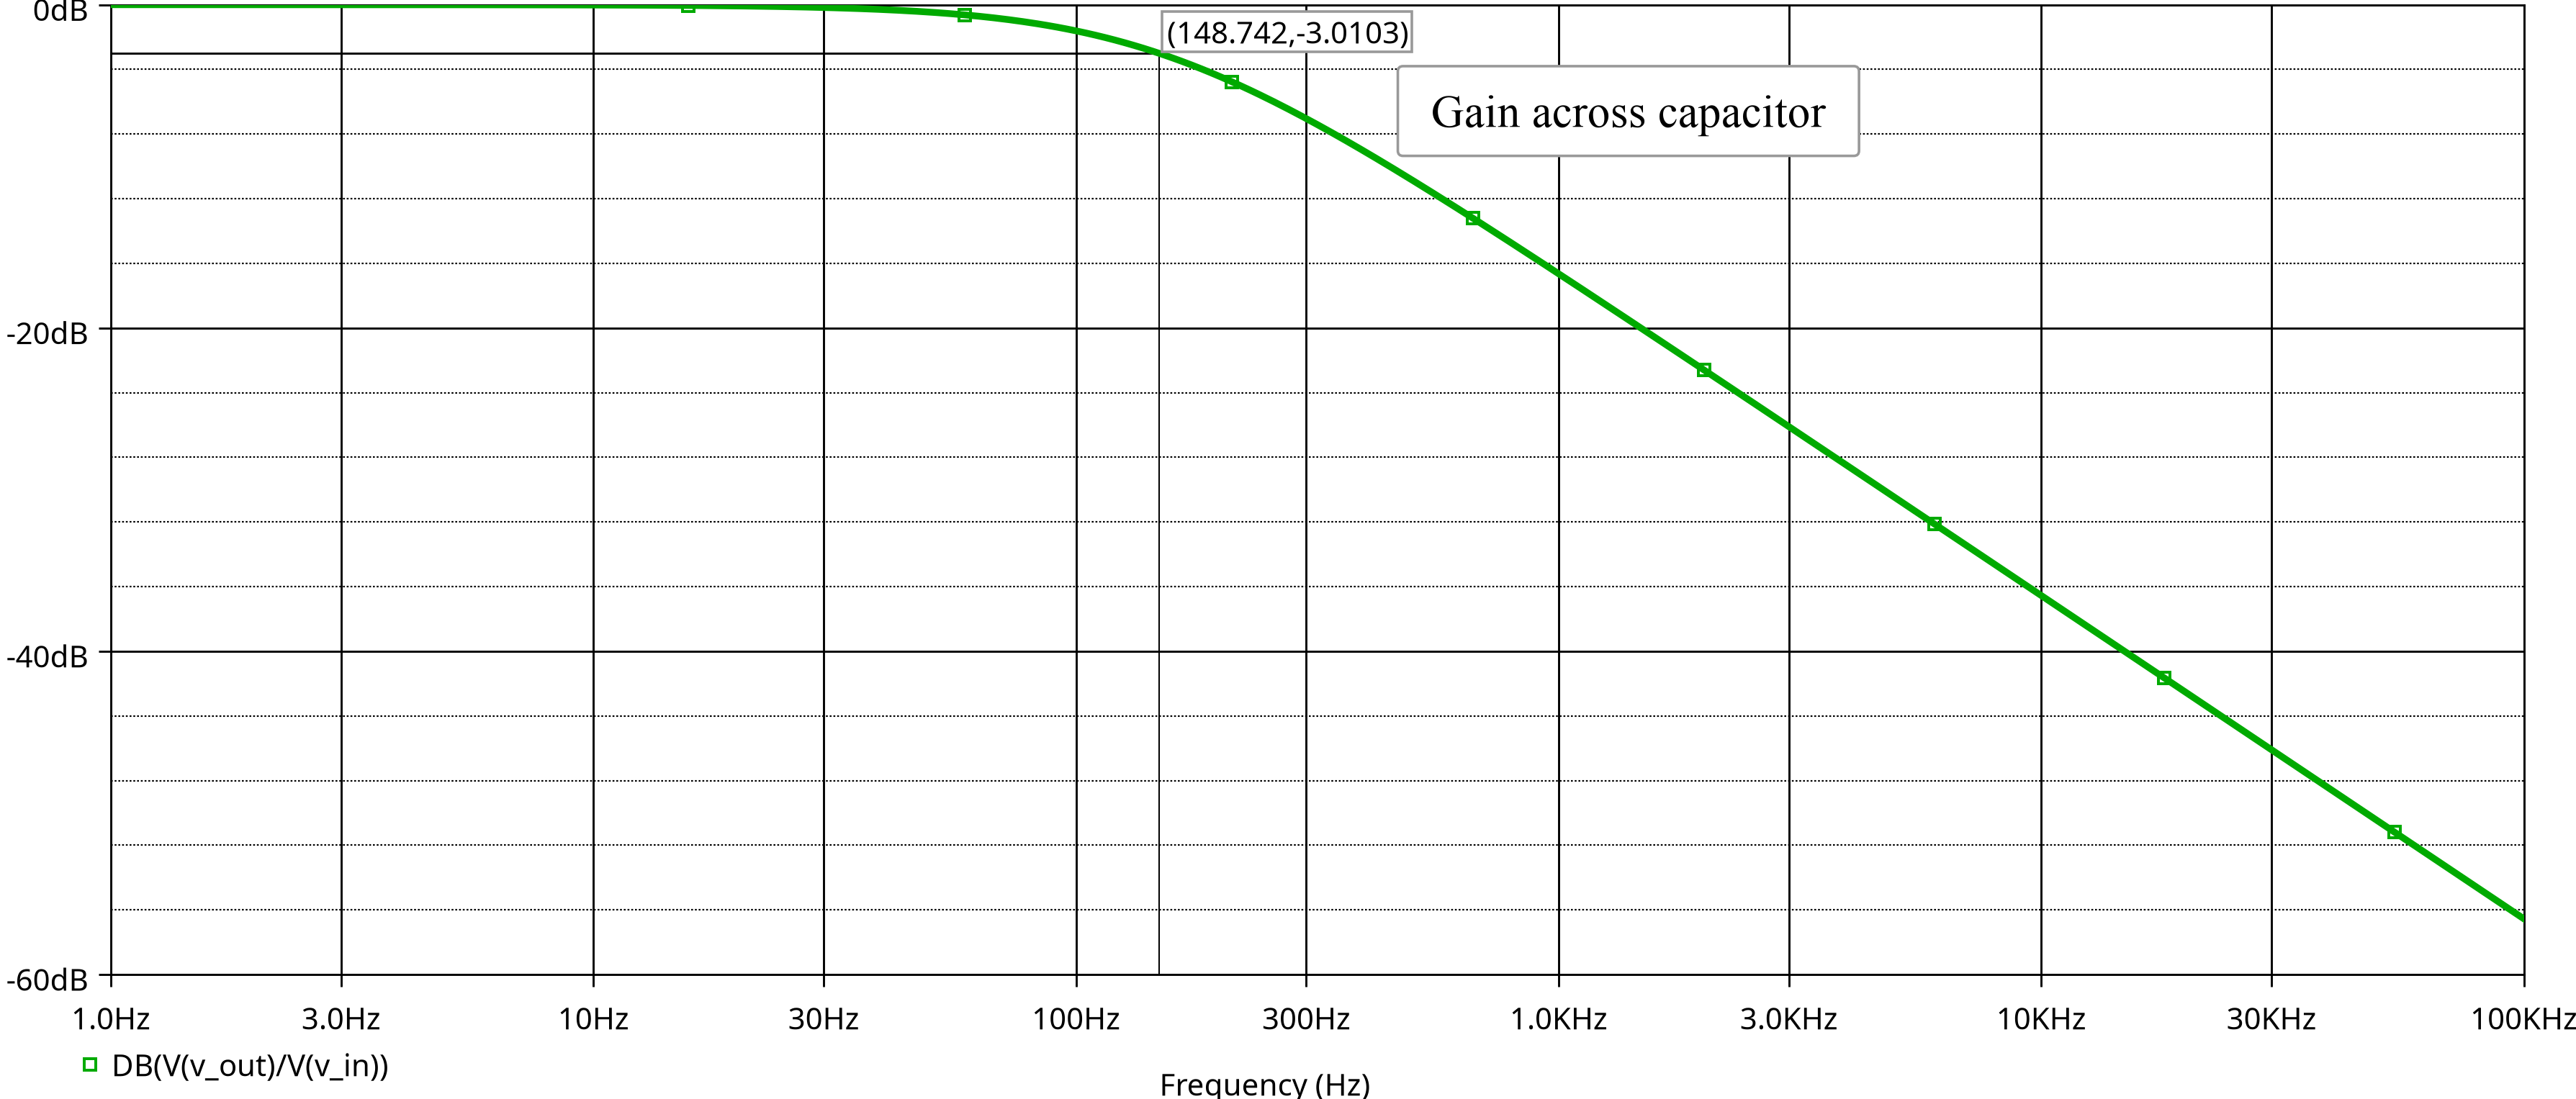
\includegraphics[width=0.95\textwidth]{pspice_graph_of_circuit1_gain_db.png}
		\caption{PSpice frequency response of the low-pass filter (circuit 1)}
		\label{fig:psp1}
	\end{figure}
	
	\begin{figure}[H]
		\centering
		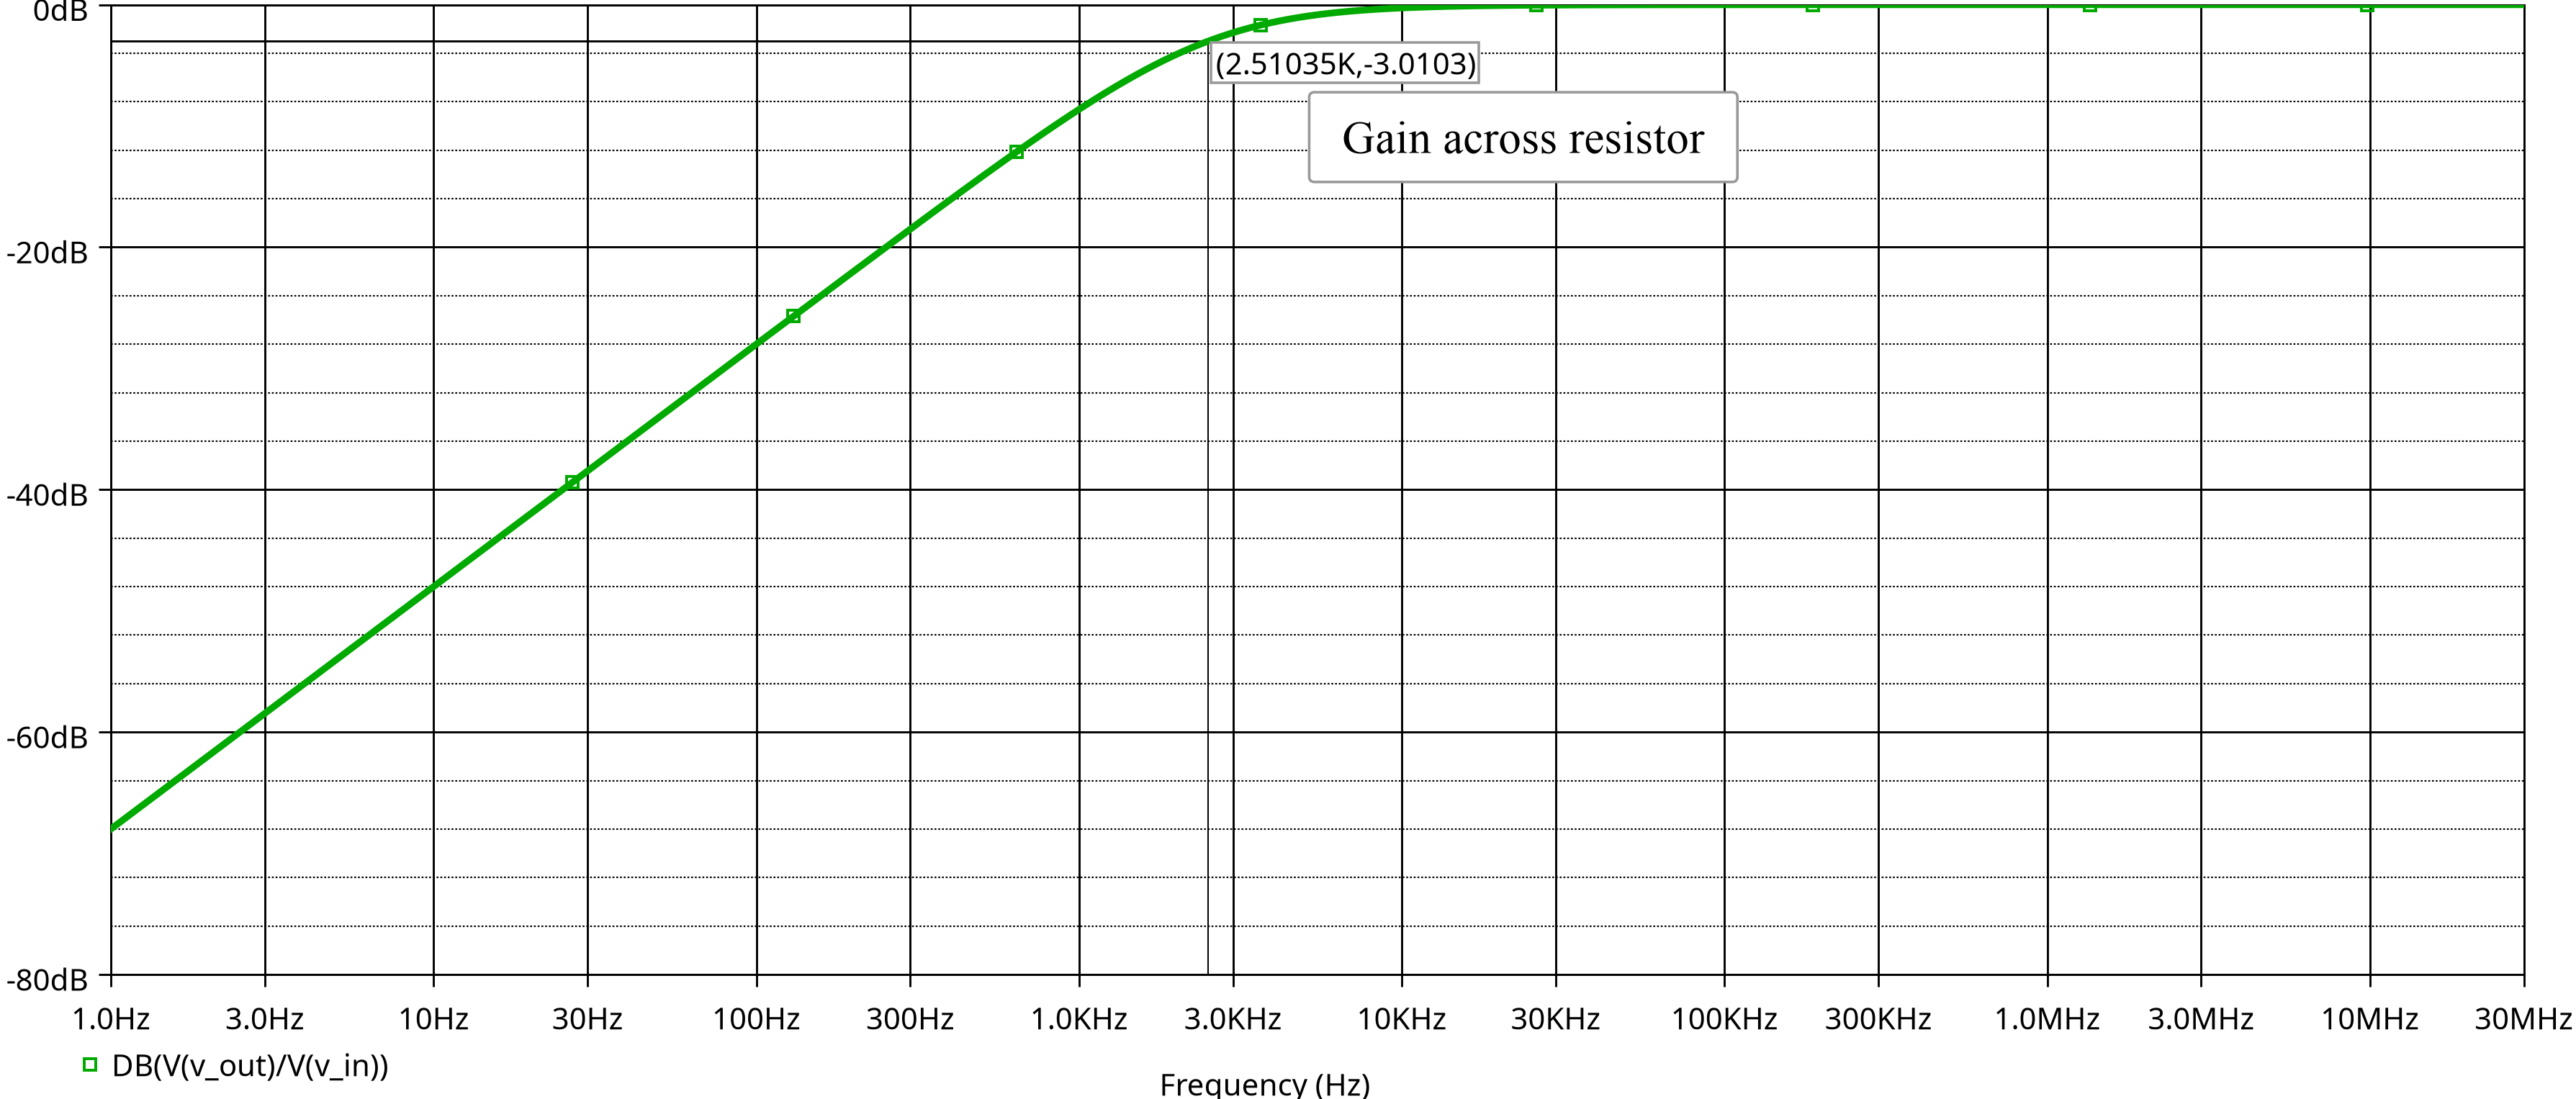
\includegraphics[width=0.95\textwidth]{pspice_graph_of_circuit2_gain_db.png}
		\caption{PSpice frequency response of the high-pass filter (circuit 2)}
		\label{fig:psp2}
	\end{figure}
	
	\begin{figure}[H]
		\centering
		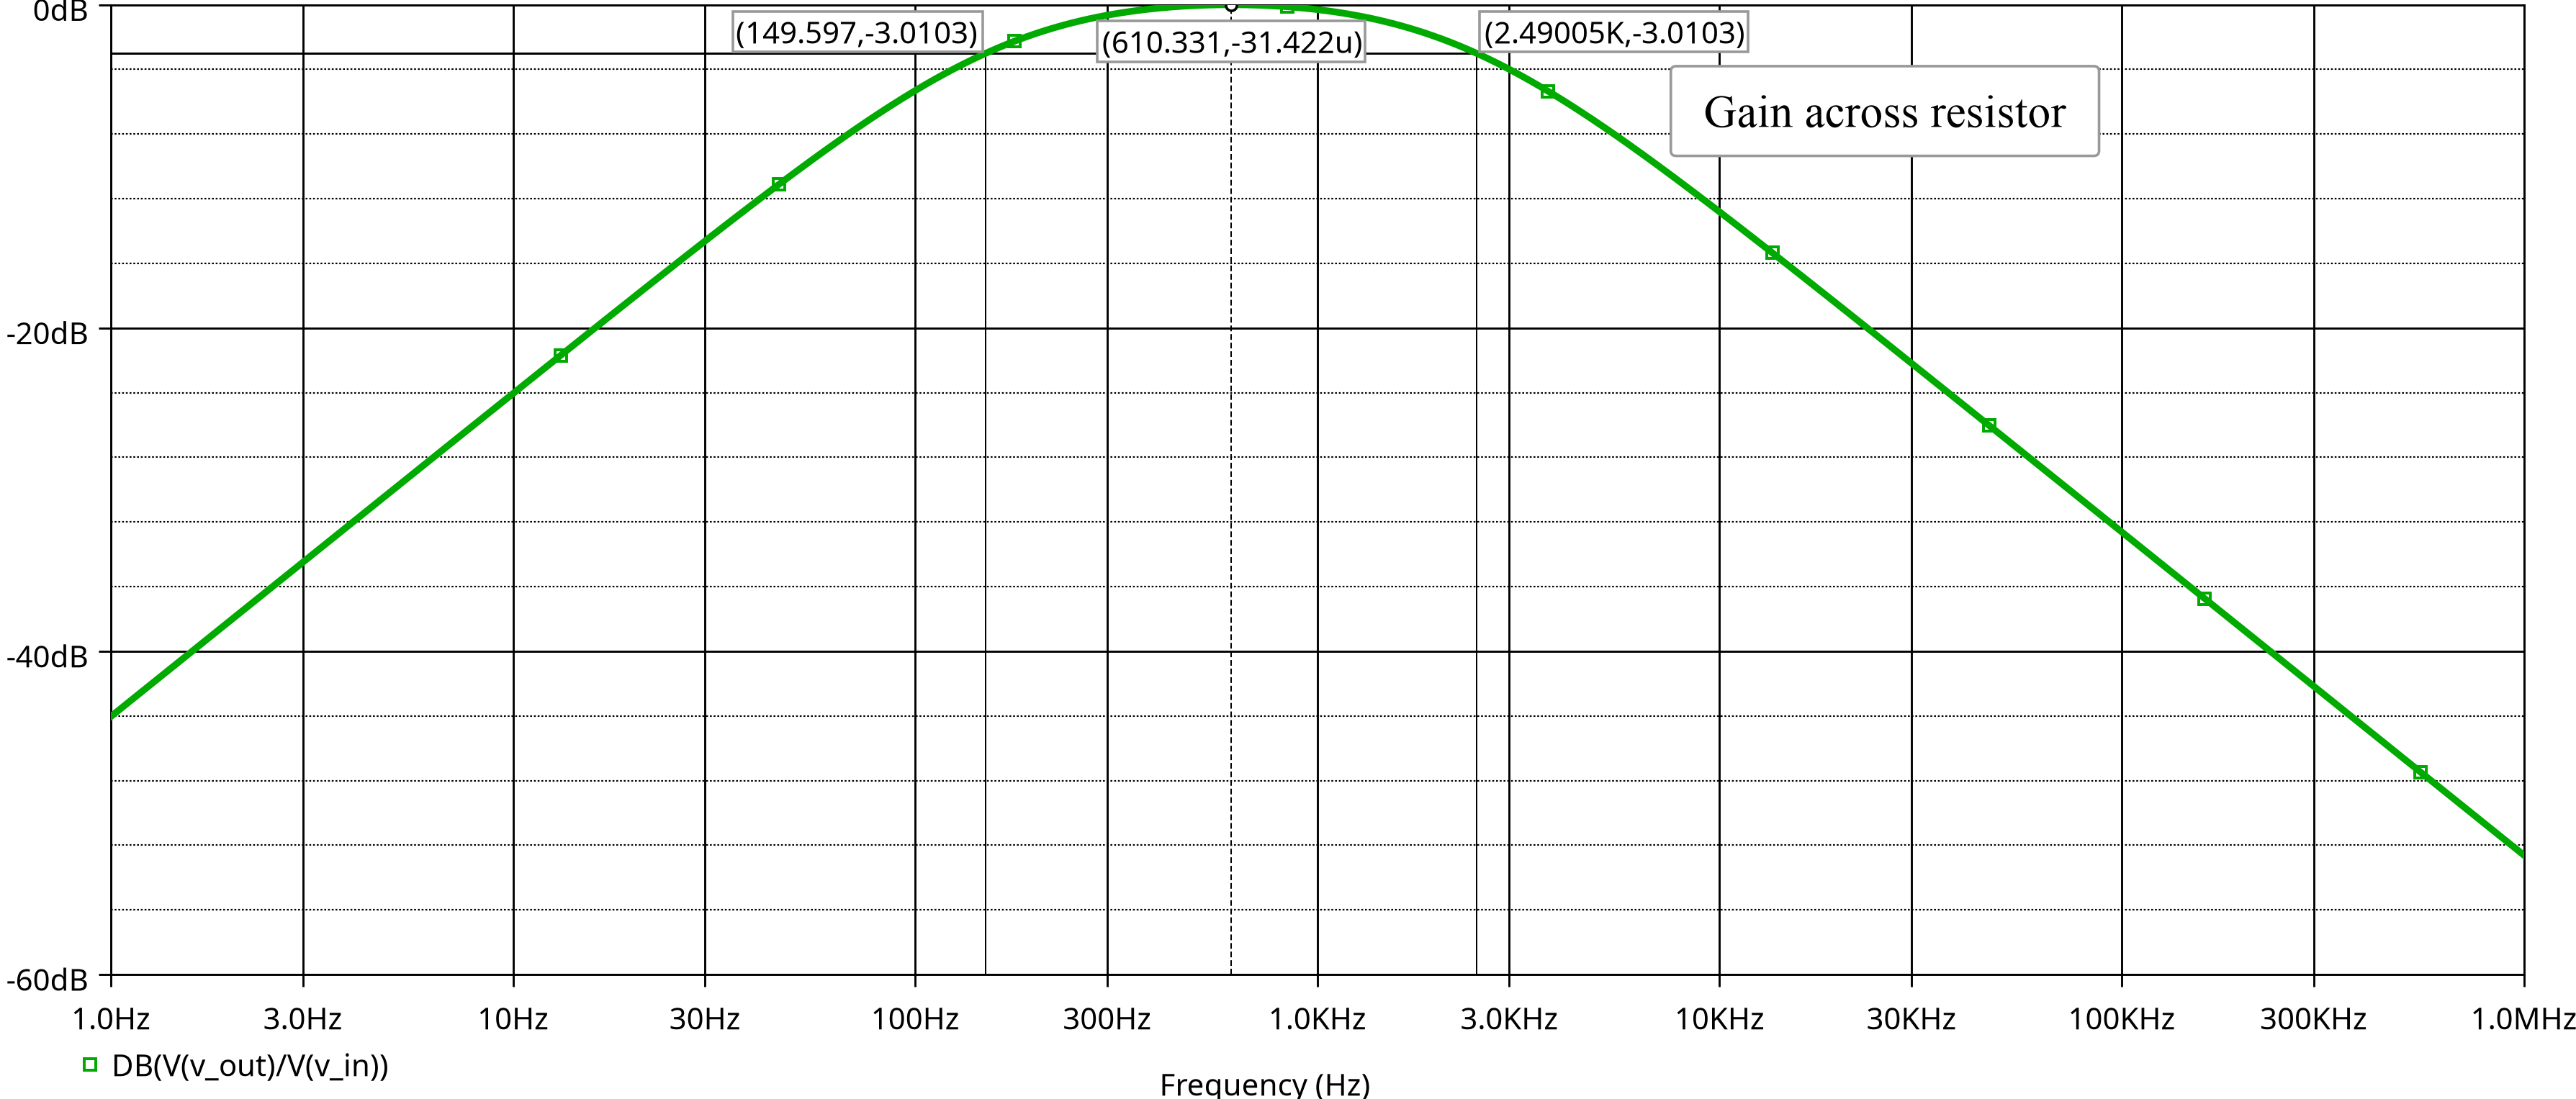
\includegraphics[width=0.95\textwidth]{pspice_graph_of_circuit3_gain_db.png}
		\caption{PSpice frequency response of the band-pass filter (circuit 3)}
		\label{fig:psp3}
	\end{figure}
	
	\begin{figure}[H]
		\centering
		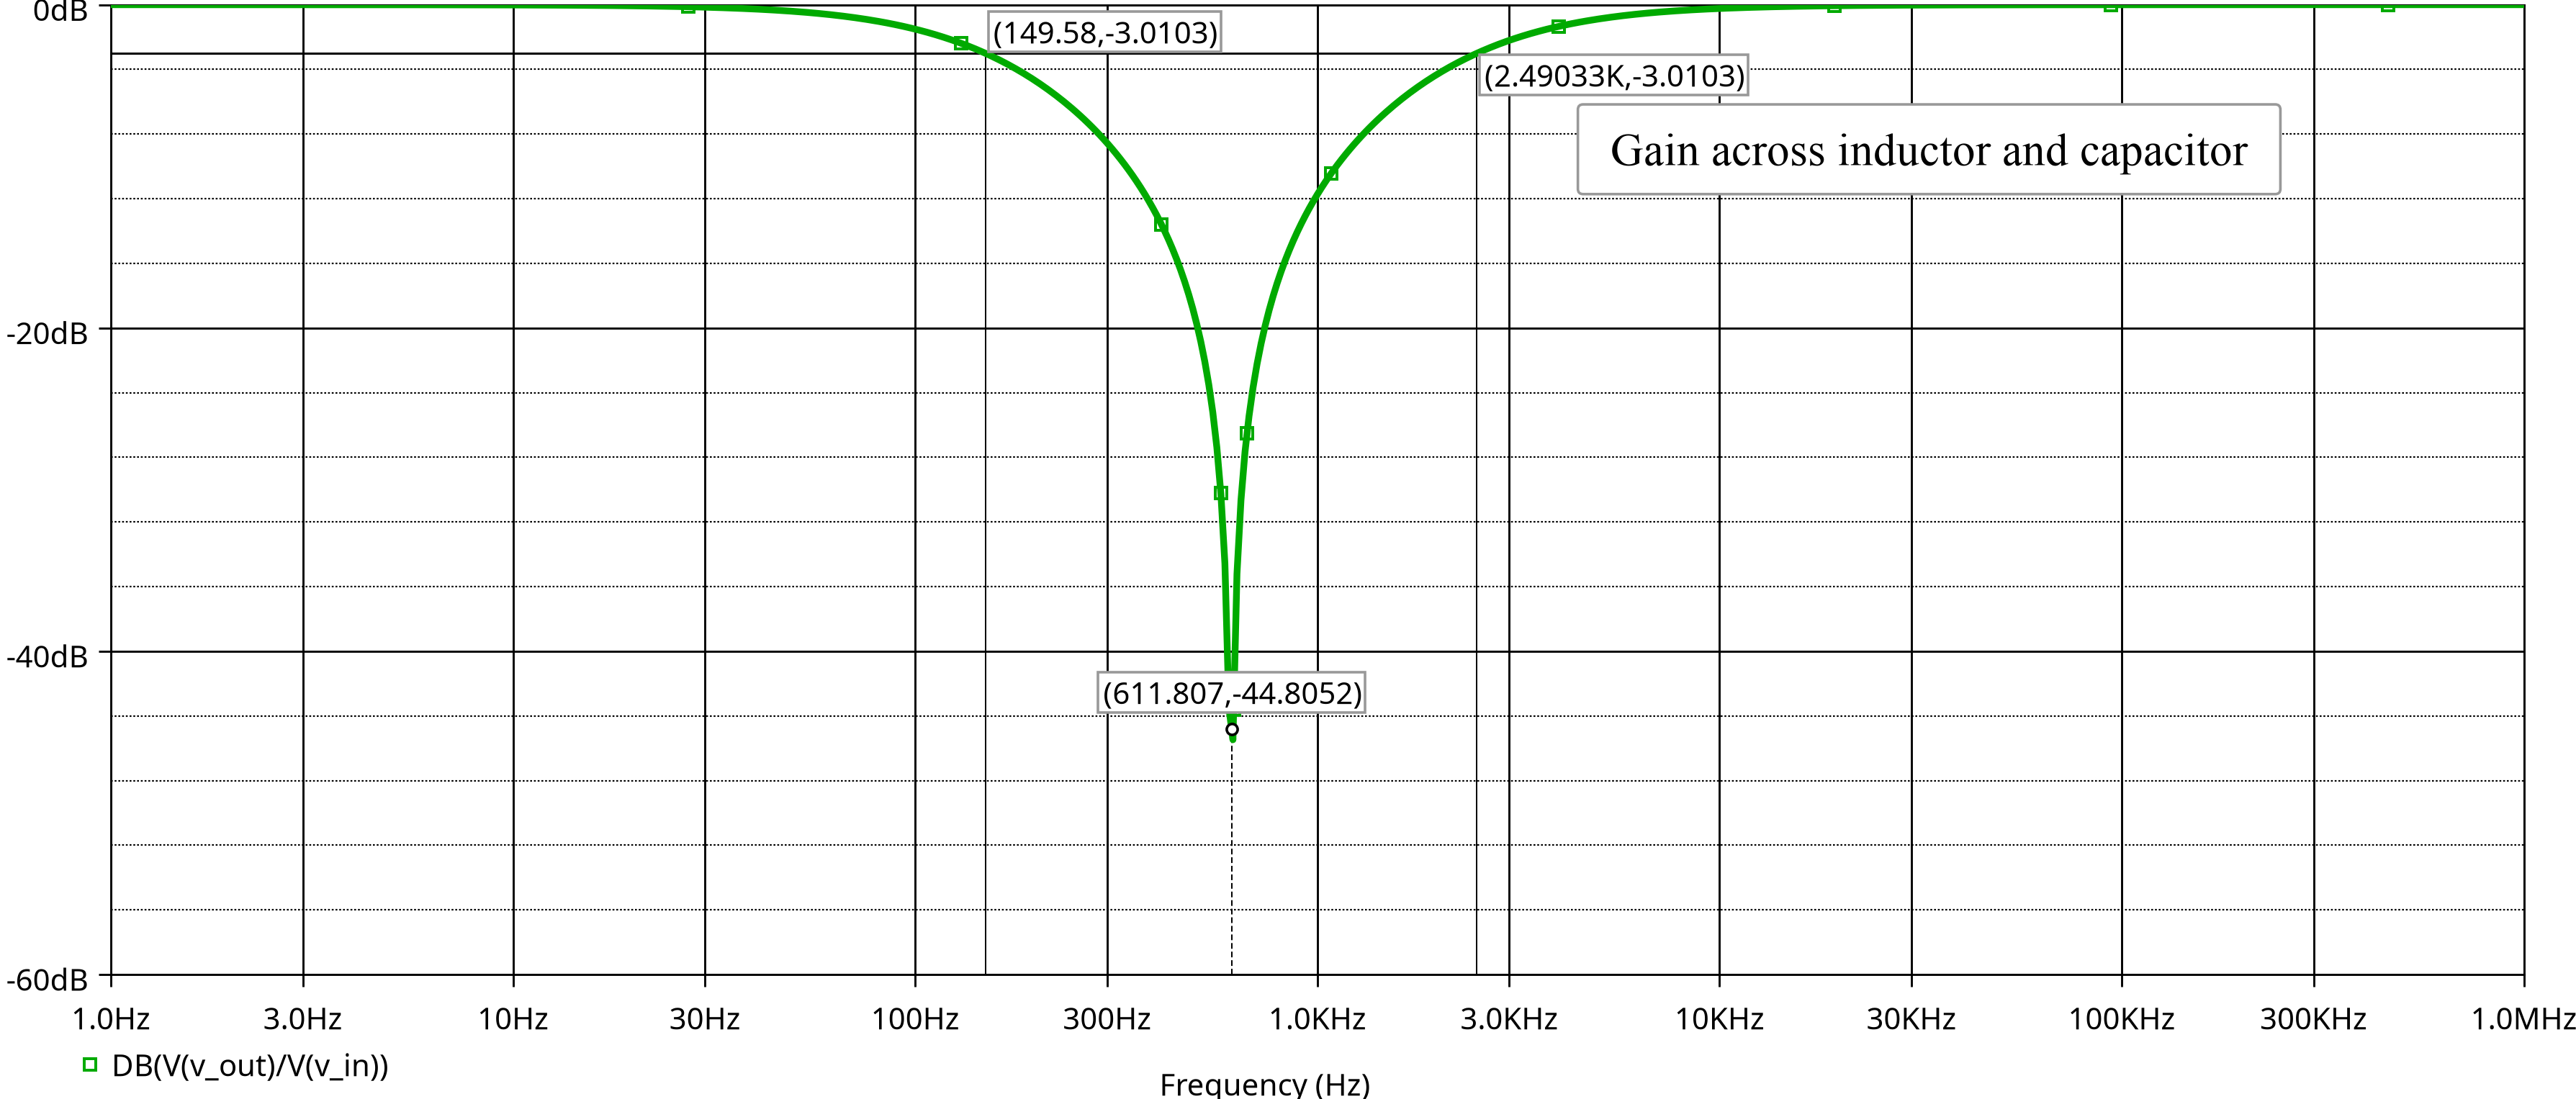
\includegraphics[width=0.95\textwidth]{pspice_graph_of_circuit4_gain_db.png}
		\caption{PSpice frequency response of the band-stop filter (circuit 4)}
		\label{fig:psp4}
	\end{figure}
	
	\begin{figure}[H]
		\centering
		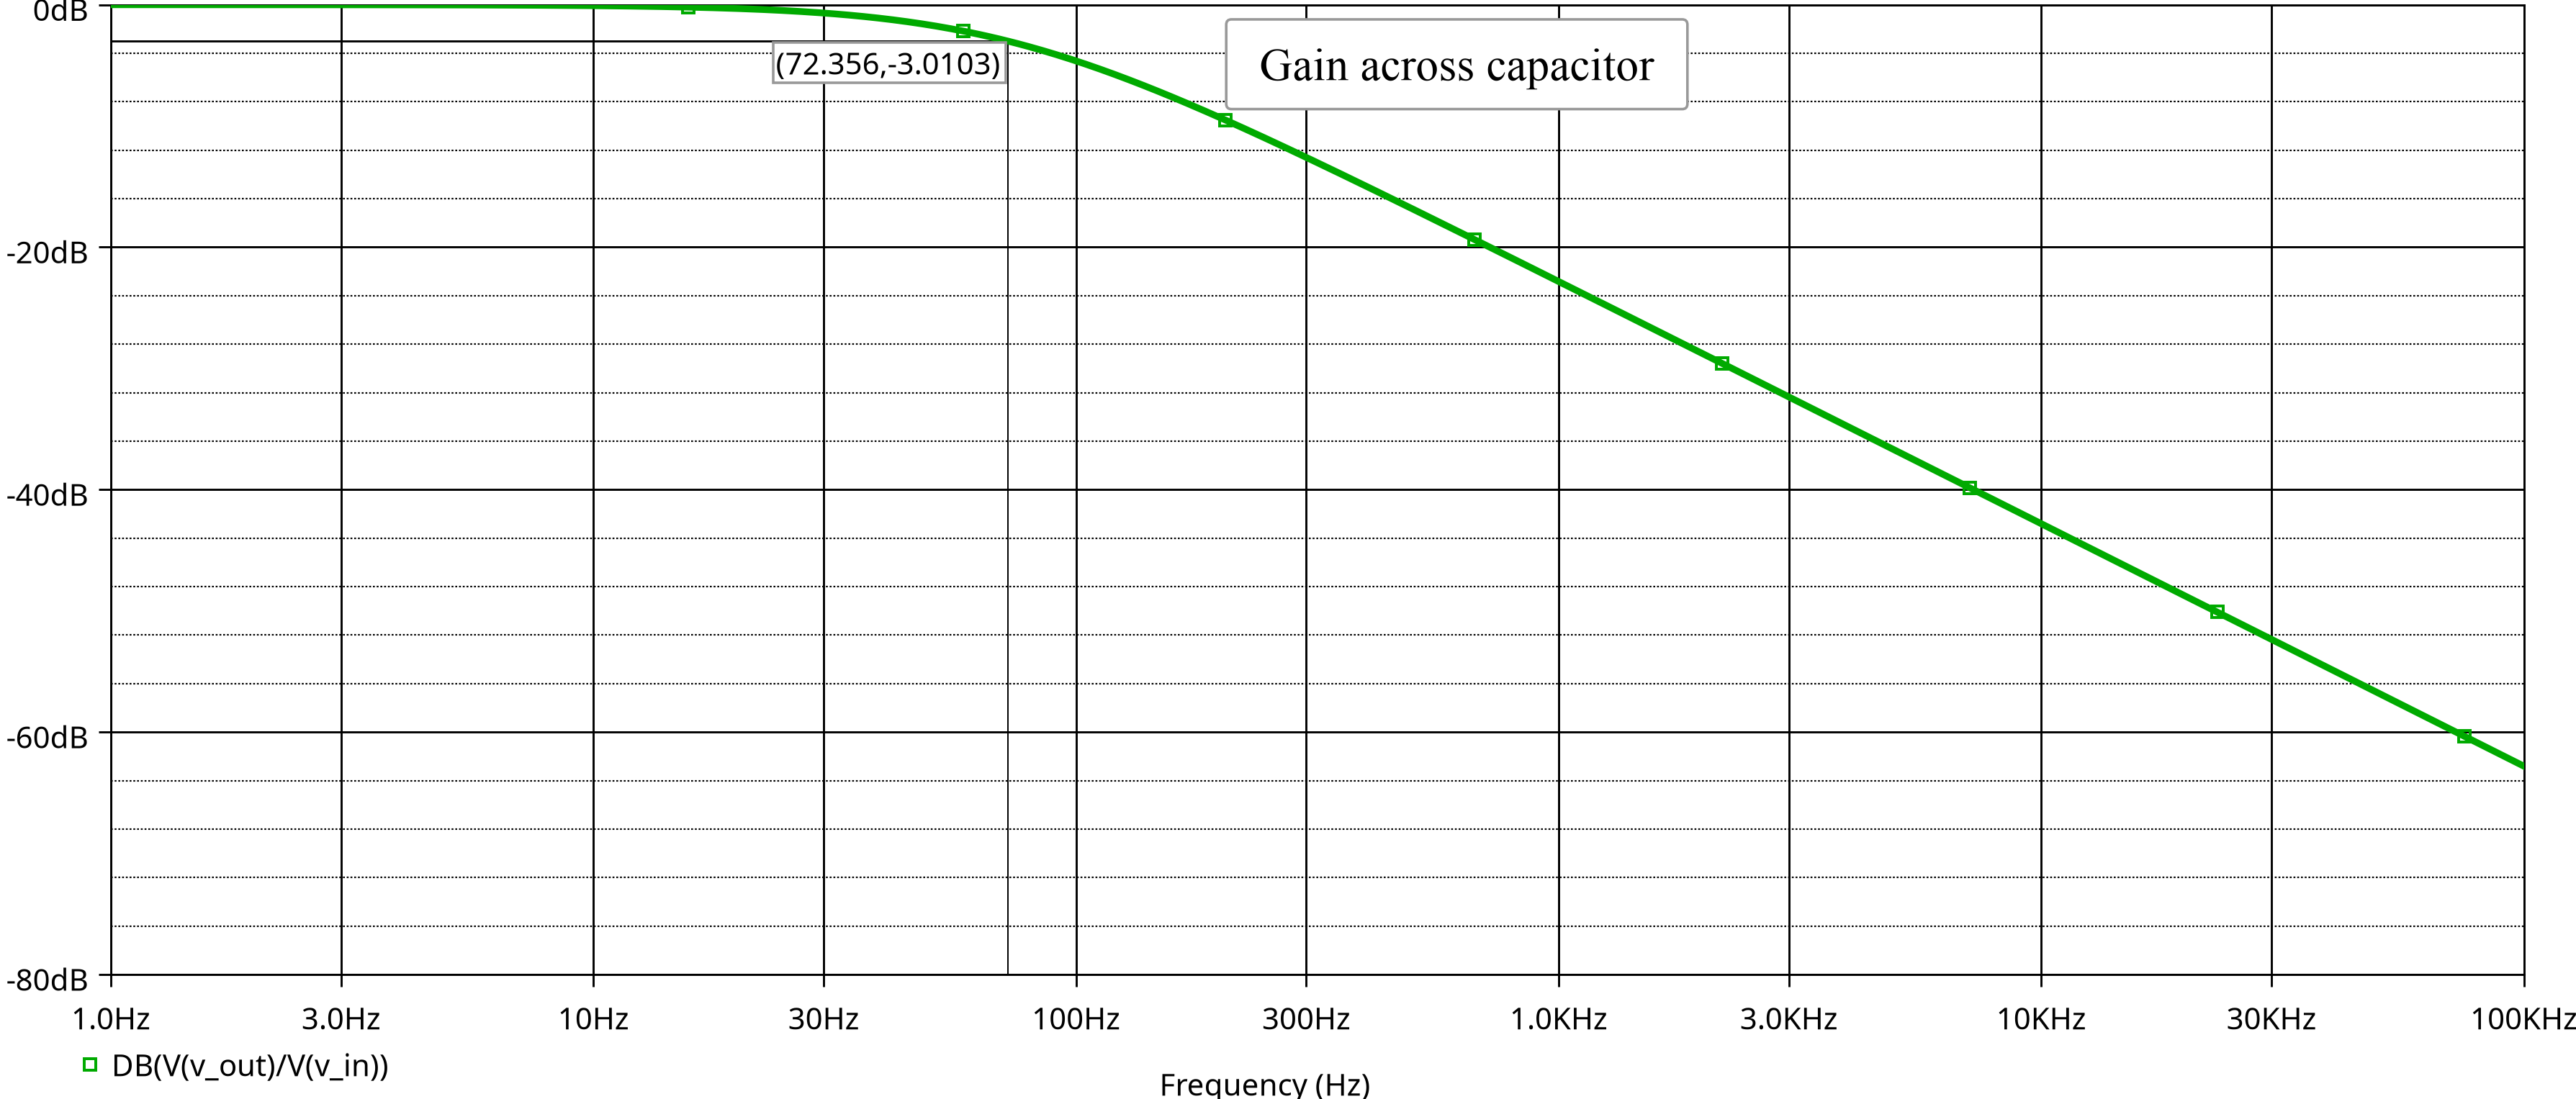
\includegraphics[width=0.95\textwidth]{pspice_graph_of_circuit1_changed_gain_db.png}
		\caption{PSpice frequency response of the modified low-pass filter
			(task 7)}
		\label{fig:pspc}
	\end{figure}
	
	\subsection{Output-voltage magnitude versus frequency}
	Figures~\ref{fig:vm1}--\ref{fig:vmc} plot the same simulations in
	absolute output voltage against frequency. The source drives the input
	with a \SI{5}{\volt} magnitude at every frequency, so each curve's
	passband level is the gain of Figures~\ref{fig:psp1}--\ref{fig:pspc} scaled by 5~V: the
	low-pass output holds near \SI{5}{\volt} at low frequency and collapses
	toward zero in the stopband; the high-pass output is complementary; the
	band-pass peaks at \SI{5}{\volt} at resonance, and the band-stop
	notches to nearly zero there ($\approx \SI{0.027}{\volt}$, i.e.\ the
	$-45.5\ \mathrm{dB}$ minimum of the sampled sweep).
	
	
	
	
	\begin{figure}[H]
		\centering
		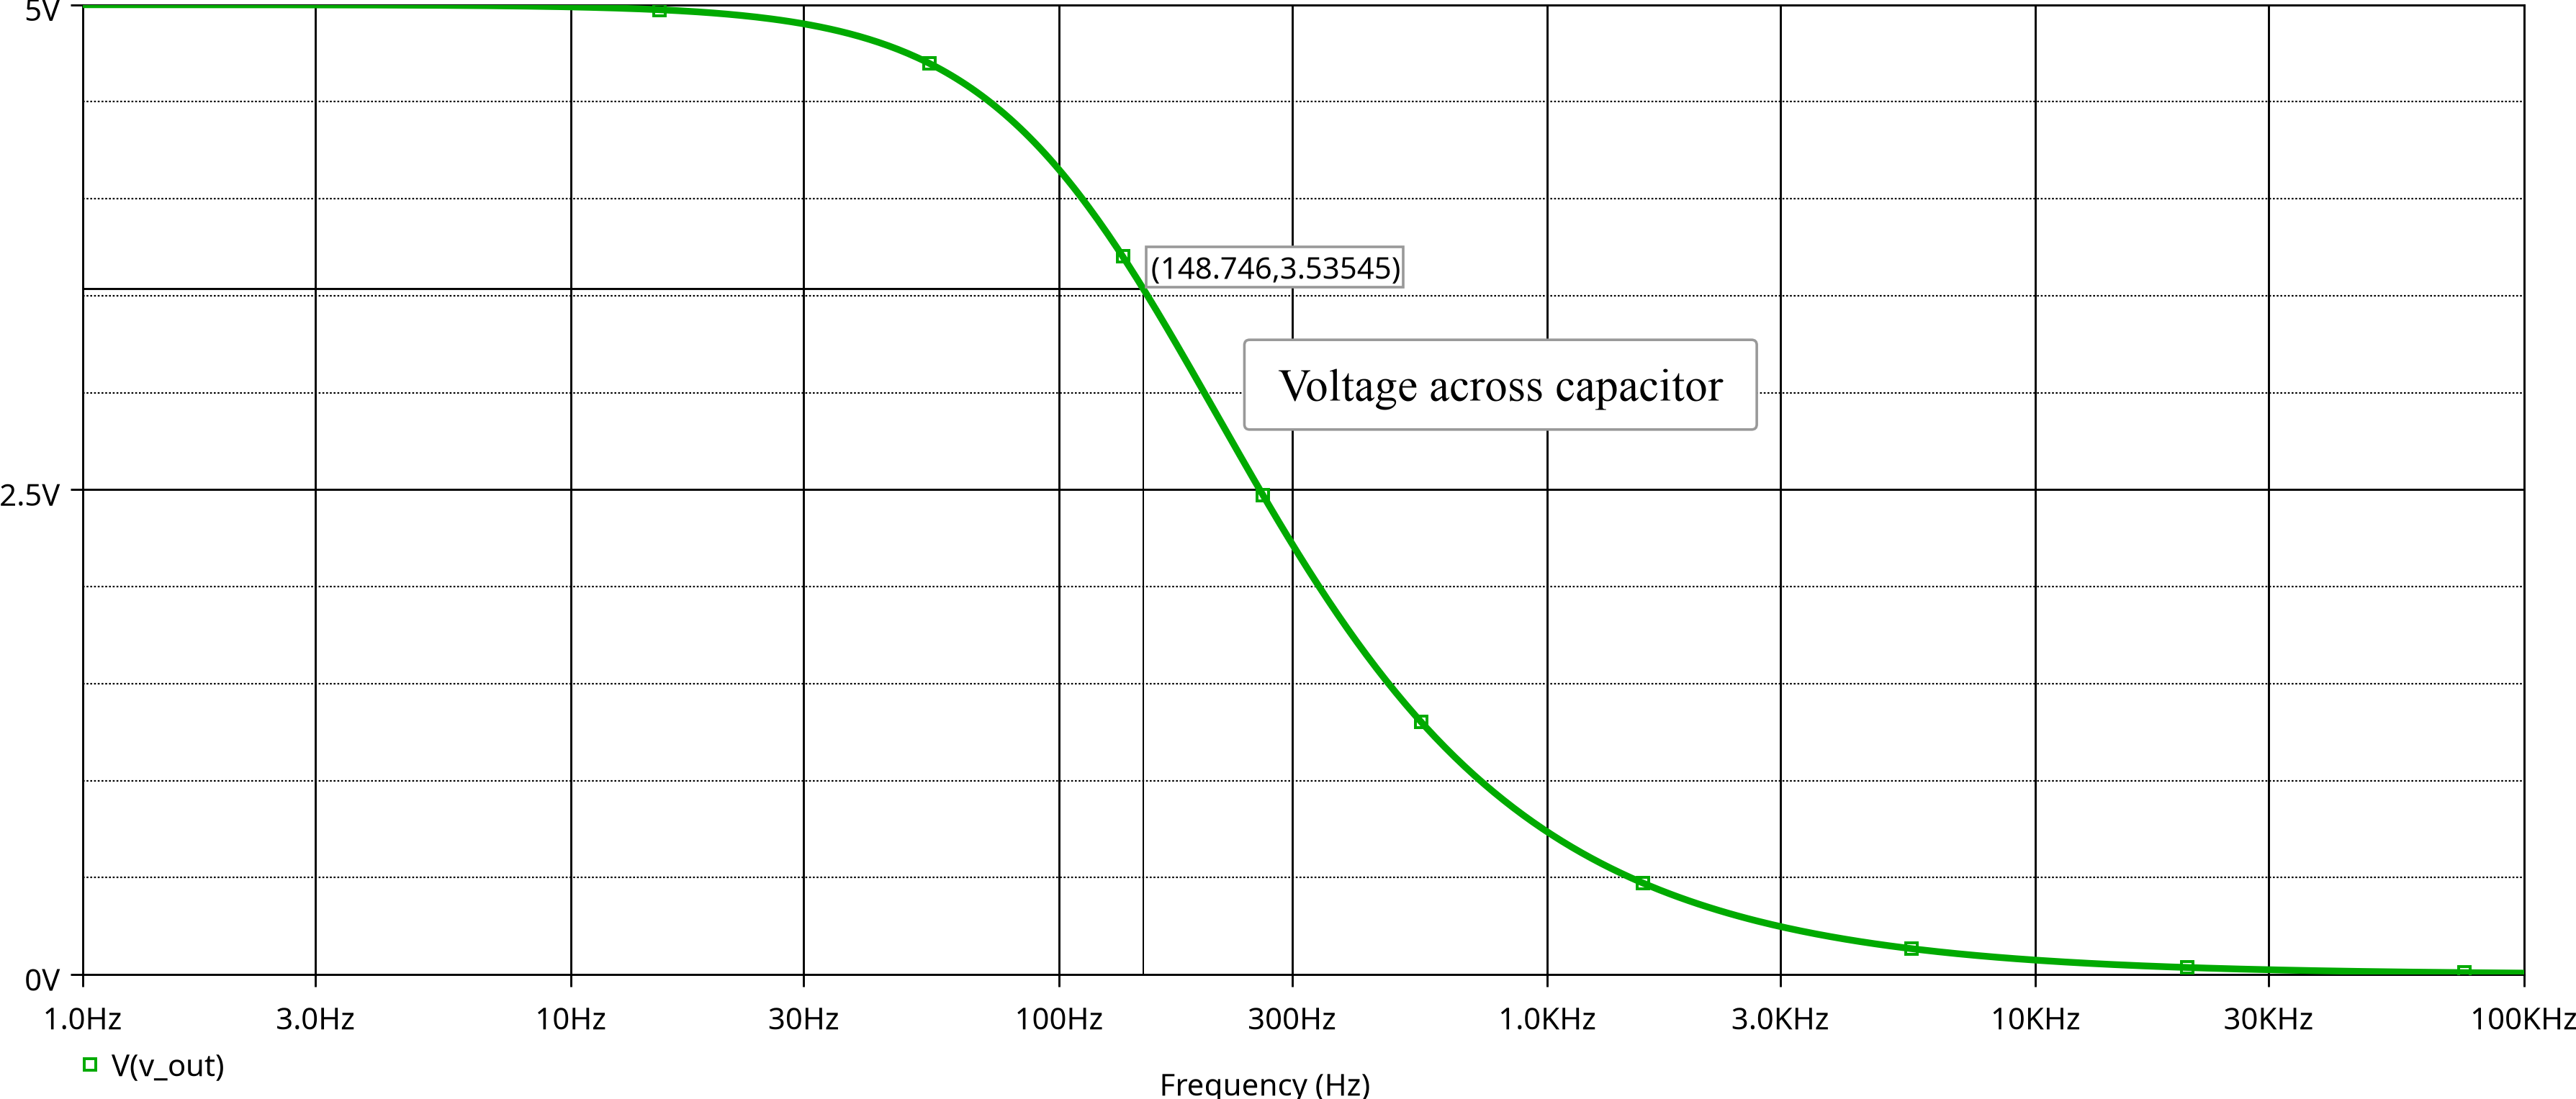
\includegraphics[width=0.95\textwidth]{pspice_graph_of_circuit1.png}
		\caption{PSpice output-voltage magnitude versus frequency for the
			low-pass filter (circuit 1)}
		\label{fig:vm1}
	\end{figure}
	
	\begin{figure}[H]
		\centering
		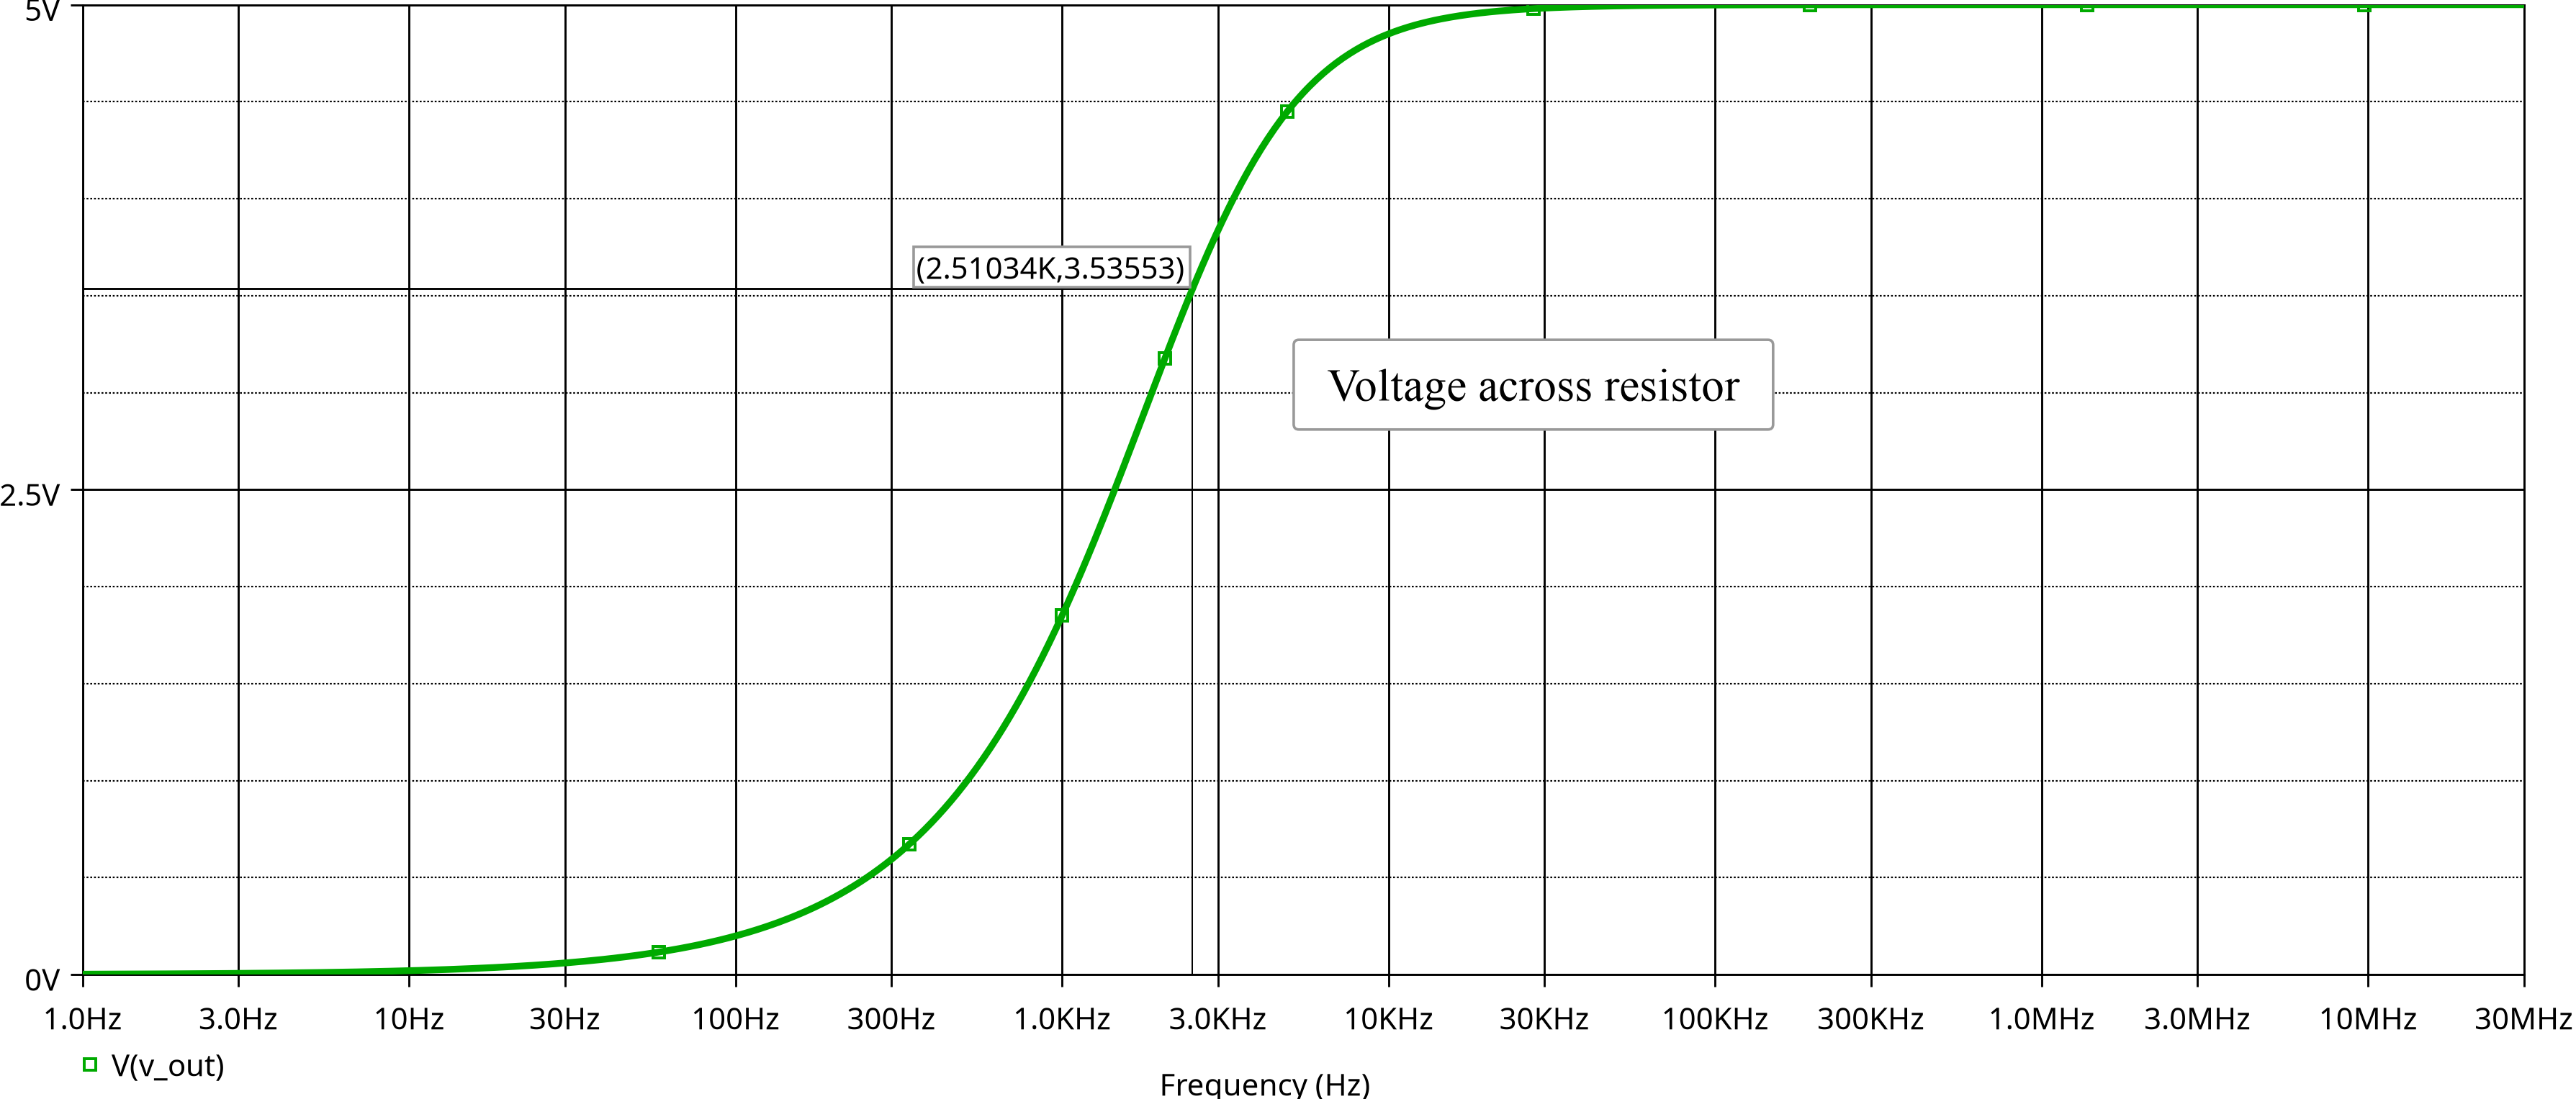
\includegraphics[width=0.95\textwidth]{pspice_graph_of_circuit2.png}
		\caption{PSpice output-voltage magnitude versus frequency for the
			high-pass filter (circuit 2)}
		\label{fig:vm2}
	\end{figure}
	
	\begin{figure}[H]
		\centering
		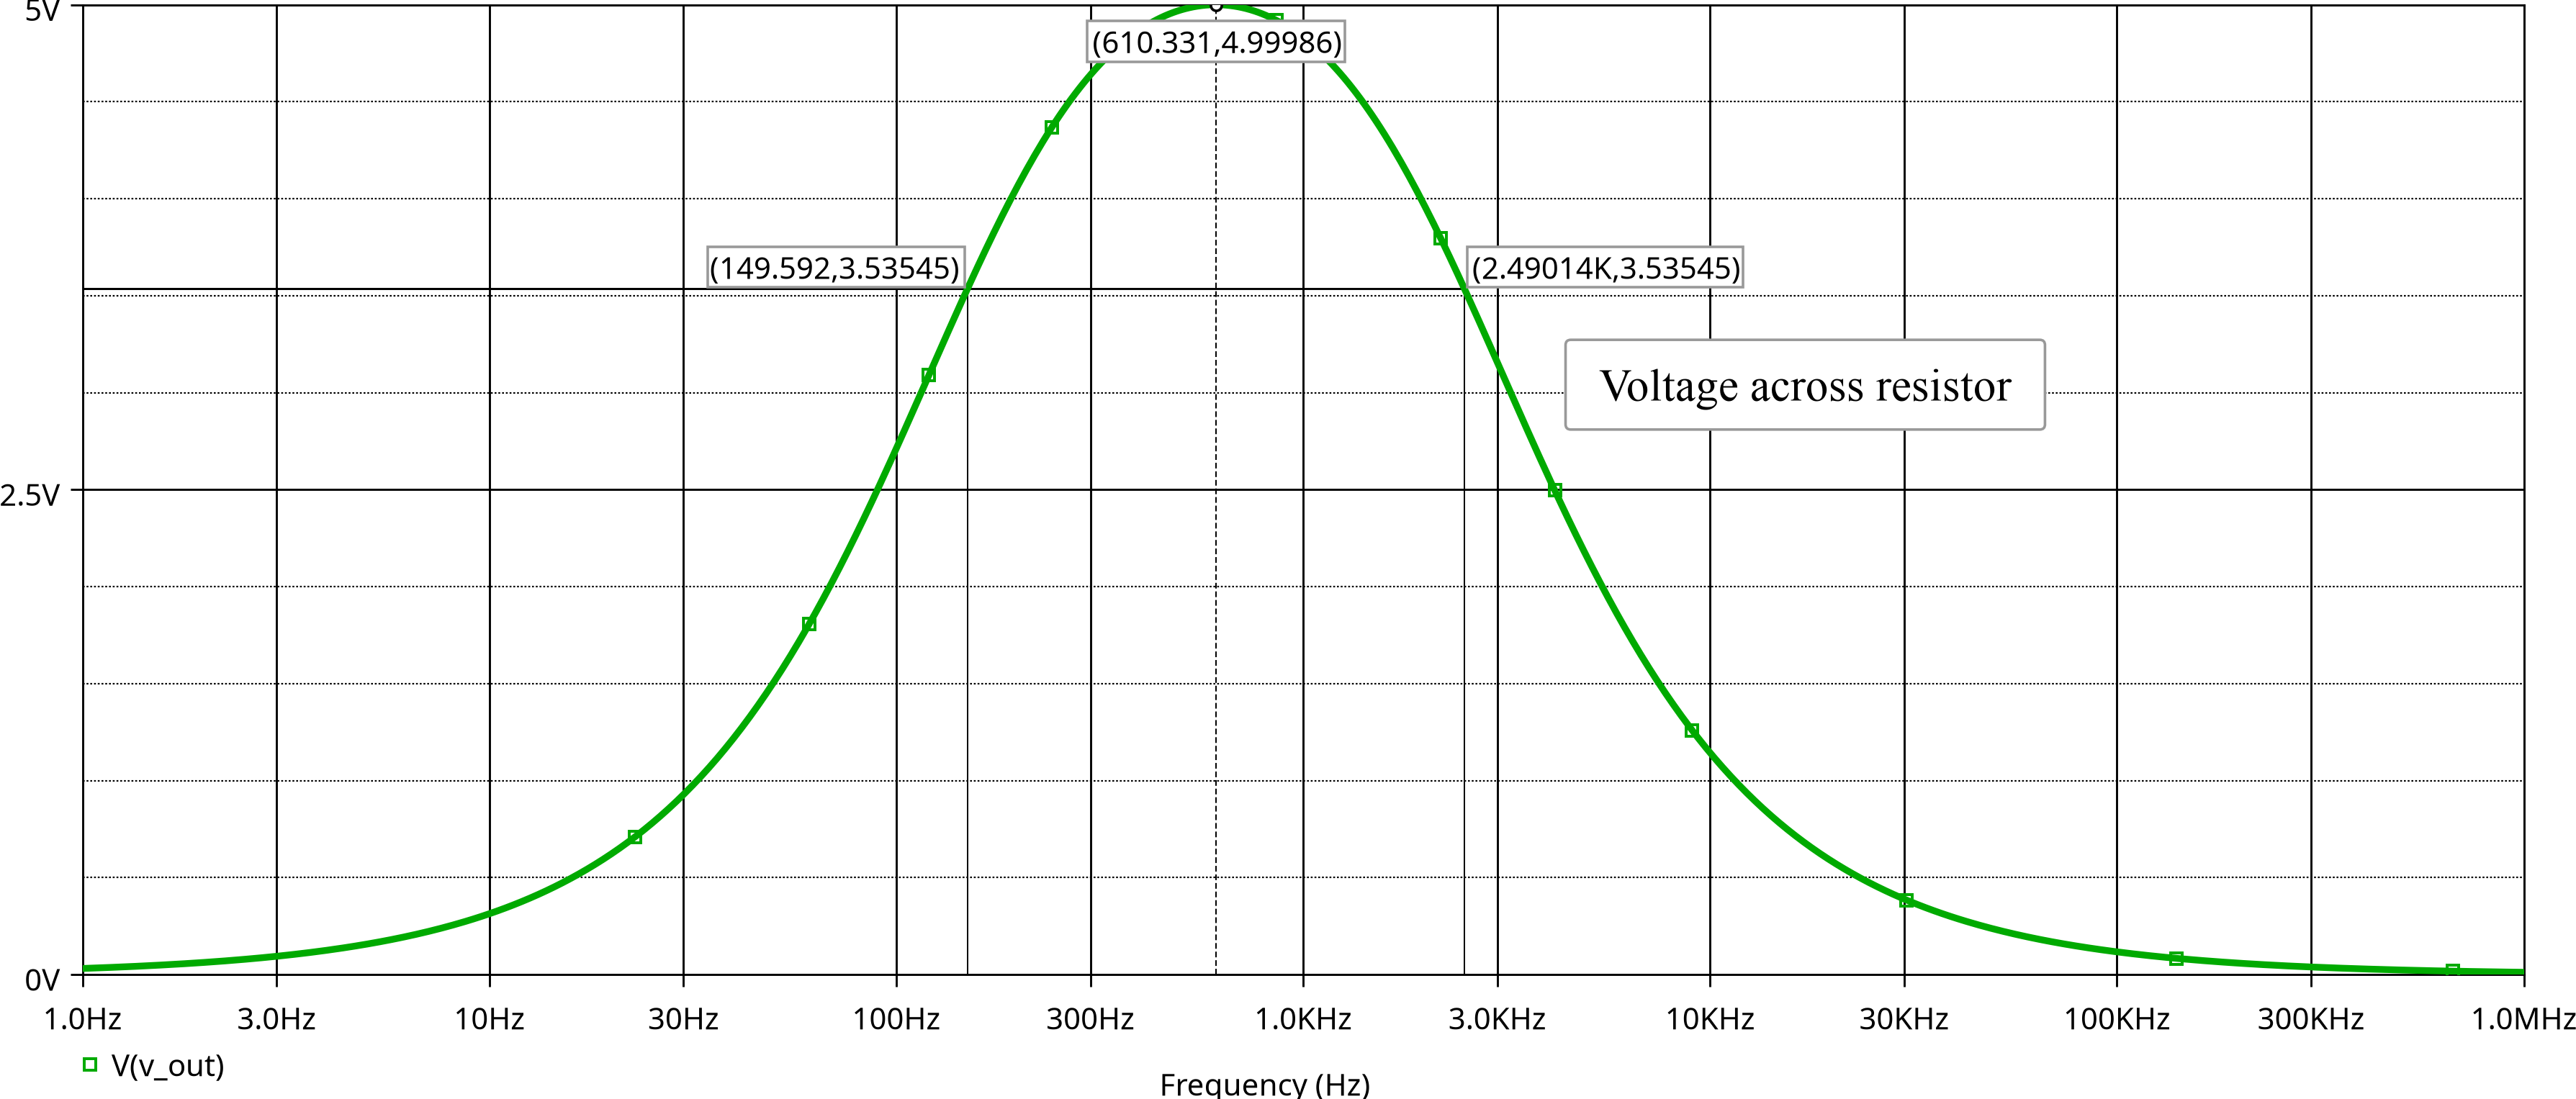
\includegraphics[width=0.95\textwidth]{pspice_graph_of_circuit3.png}
		\caption{PSpice output-voltage magnitude versus frequency for the
			band-pass filter (circuit 3)}
		\label{fig:vm3}
	\end{figure}
	
	\begin{figure}[H]
		\centering
		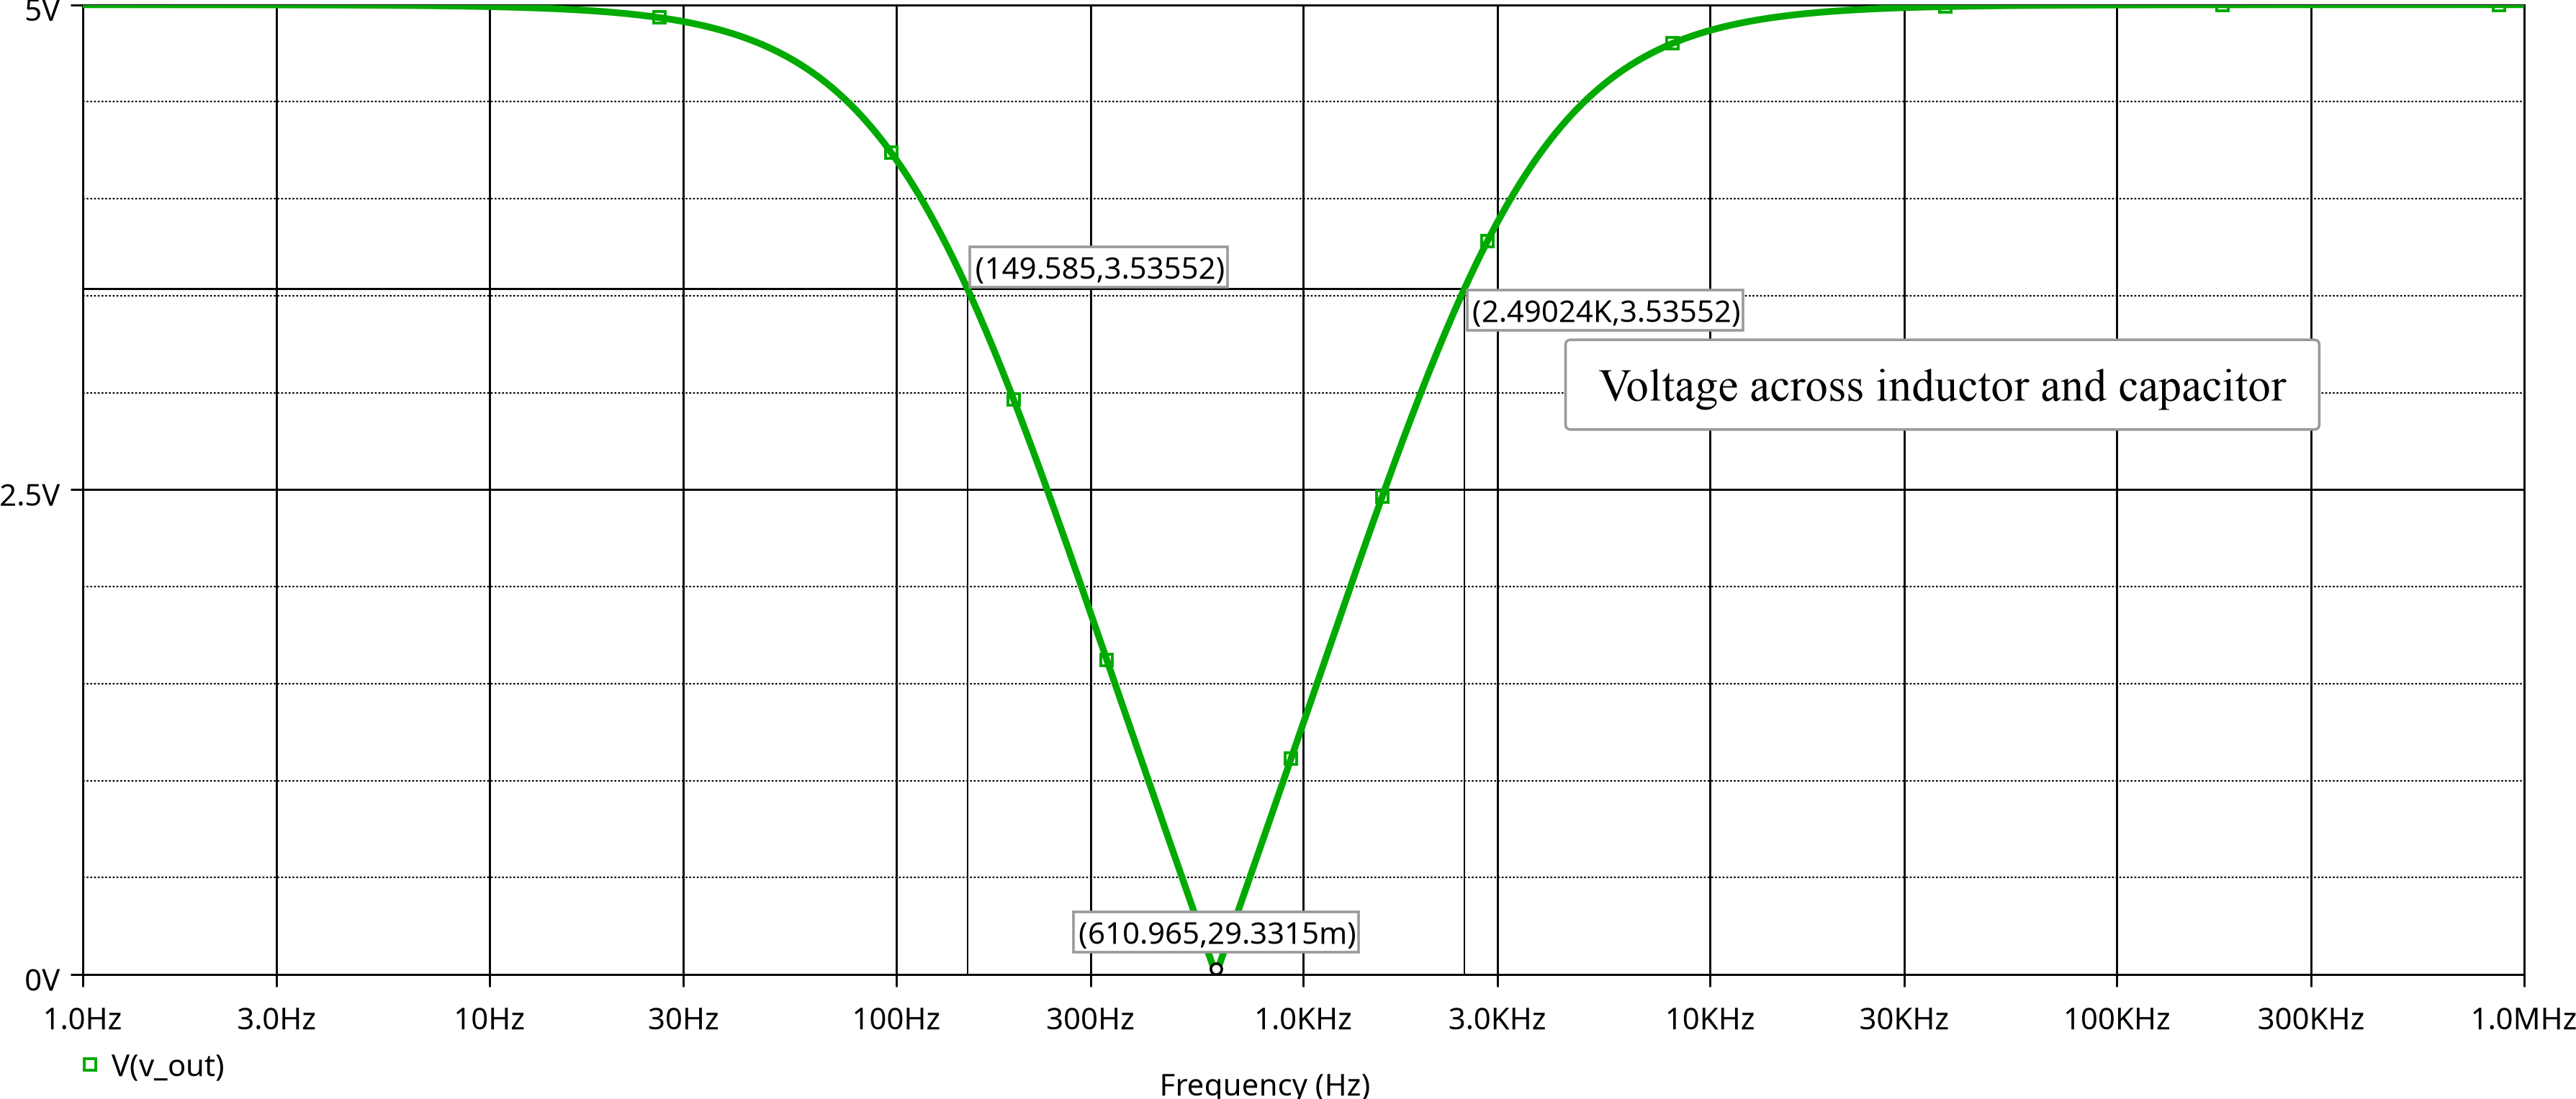
\includegraphics[width=0.95\textwidth]{pspice_graph_of_circuit4.png}
		\caption{PSpice output-voltage magnitude versus frequency for the
			band-stop filter (circuit 4)}
		\label{fig:vm4}
	\end{figure}
	
	\begin{figure}[H]
		\centering
		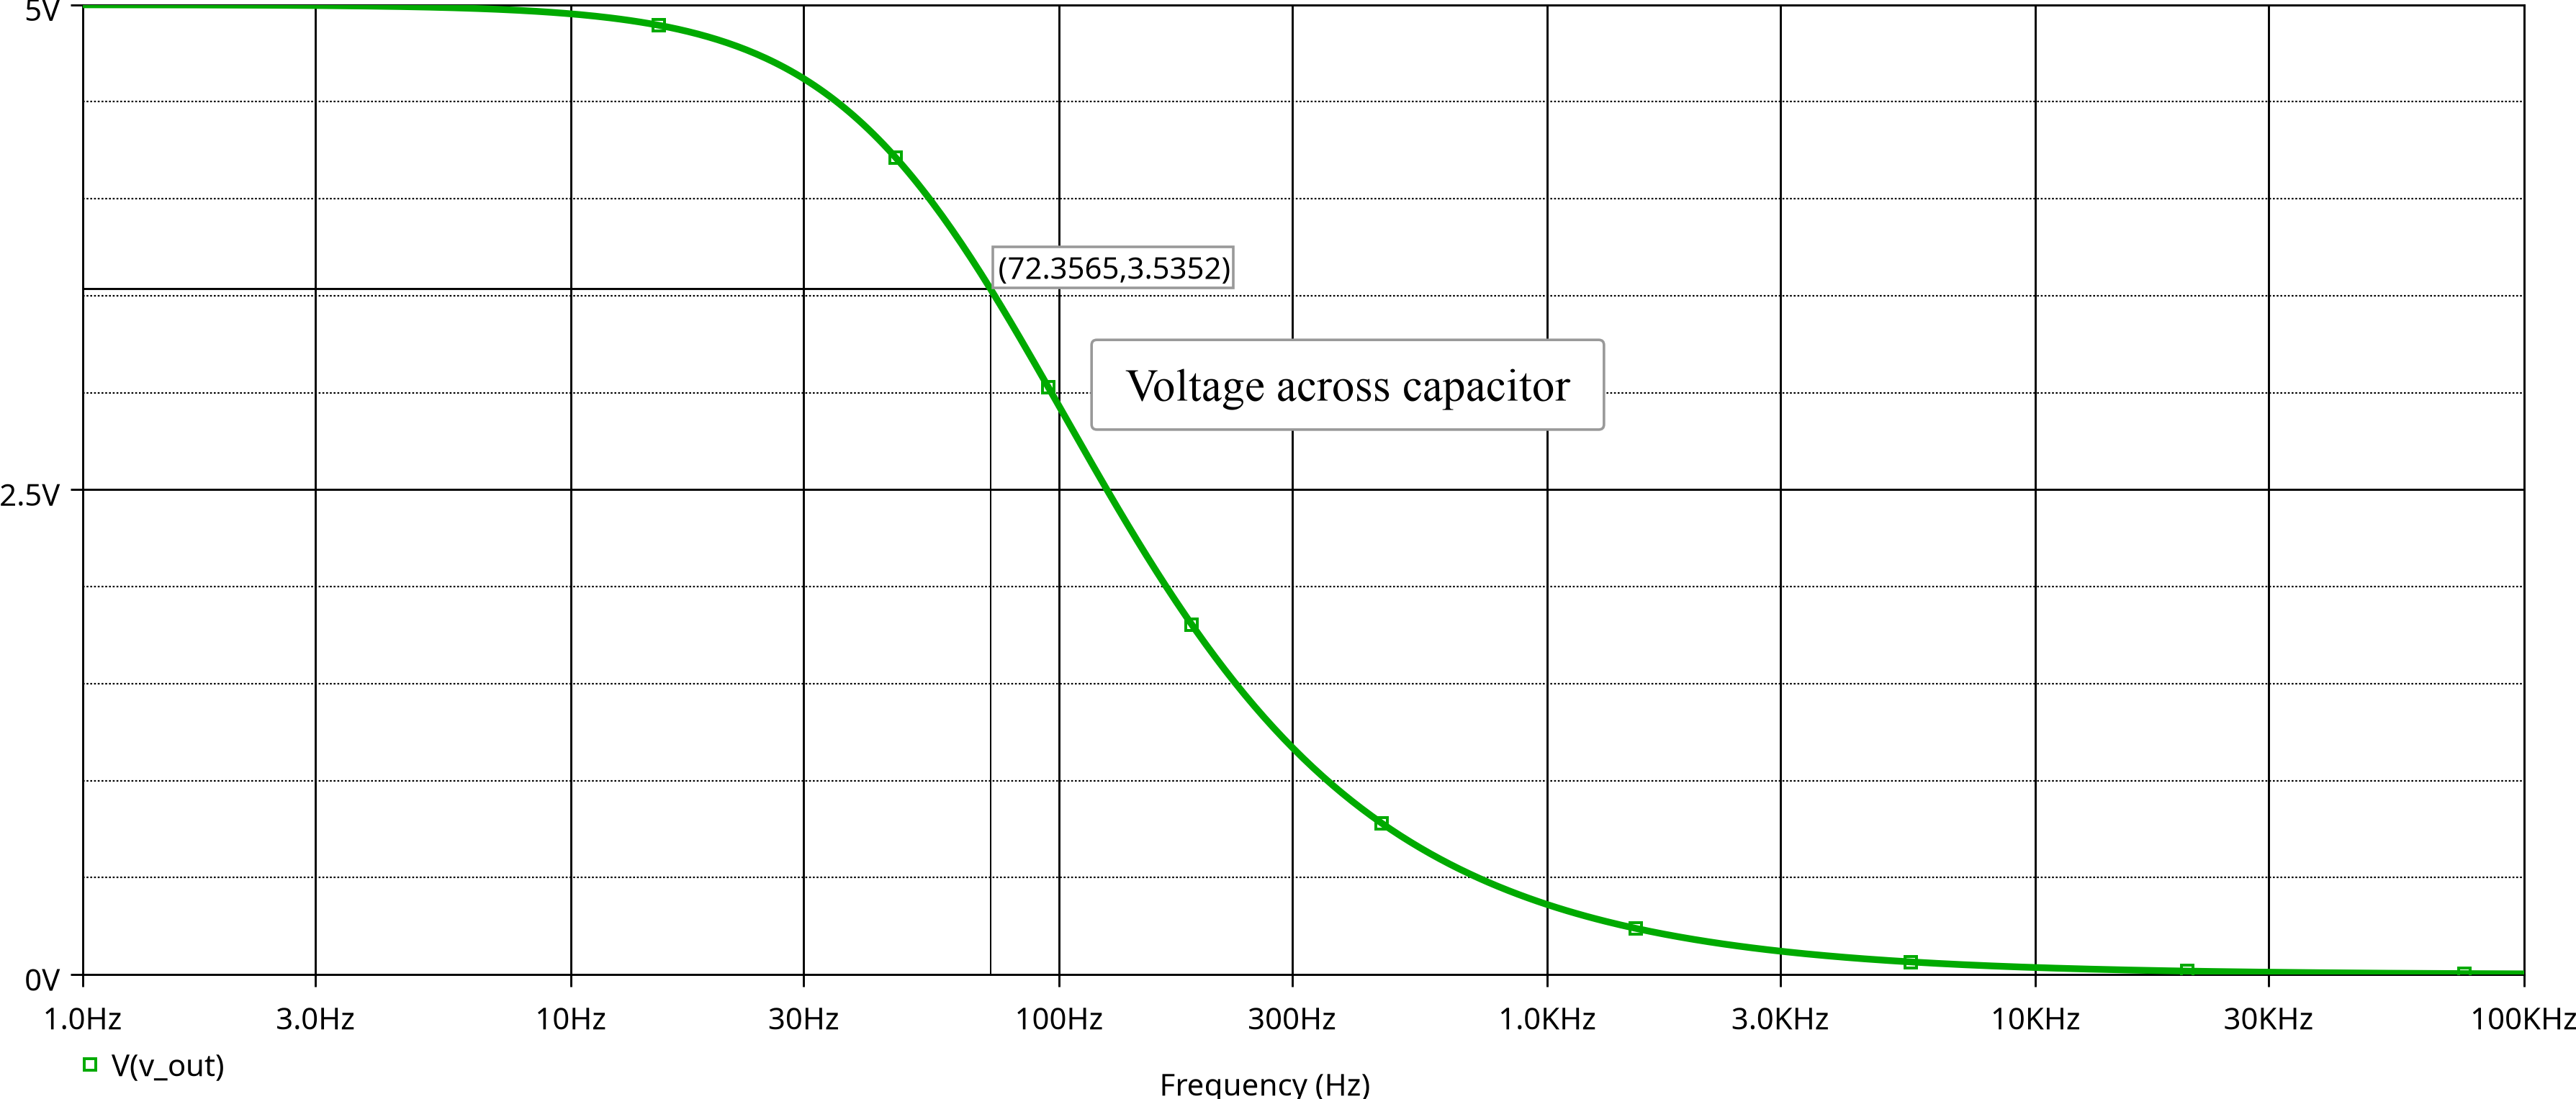
\includegraphics[width=0.95\textwidth]{pspice_graph_of_circuit1_changed.png}
		\caption{PSpice output-voltage magnitude versus frequency for the
			modified low-pass filter (task 7)}
		\label{fig:vmc}
	\end{figure}
	
	Tables~\ref{tab:data1}--\ref{tab:datac} list the data points read off the
	traces of Figures~\ref{fig:vm1}--\ref{fig:vmc}, from which the
	characteristic frequencies were determined using the 70.7\%
	criterion:
	
	\begin{table}[H]
		\centering
		\caption{Data points read off the PSpice trace of the low-pass filter}
		\label{tab:data1}
		\small
		\renewcommand{\arraystretch}{1.2}
		\begin{tabular}{|c|c|c|c|}
			\hline
			\rowcolor{black!12}\textbf{Input voltage $|V_{\mathrm{in}}|$ (V)} & \textbf{Frequency (Hz)} & \textbf{Output voltage $|V_{\mathrm{out}}|$ (V)} & \textbf{Gain $A_v = |V_{\mathrm{out}}|/|V_{\mathrm{in}}|$} \\
			\hline
			\num{5.000} & \num{1.00} & \num{5.000} & \num{1.0000}\\
			\hline
			\num{5.000} & \num{14.79} & \num{4.975} & \num{0.9950}\\
			\hline
			\num{5.000} & \num{26.30} & \num{4.924} & \num{0.9848}\\
			\hline
			\num{5.000} & \num{40.74} & \num{4.822} & \num{0.9644}\\
			\hline
			\num{5.000} & \num{50.12} & \num{4.738} & \num{0.9476}\\
			\hline
			\num{5.000} & \num{60.26} & \num{4.634} & \num{0.9268}\\
			\hline
			\num{5.000} & \num{70.79} & \num{4.515} & \num{0.9030}\\
			\hline
			\num{5.000} & \num{83.18} & \num{4.364} & \num{0.8728}\\
			\hline
			\num{5.000} & \num{97.72} & \num{4.179} & \num{0.8358}\\
			\hline
			\num{5.000} & \num{112.20} & \num{3.992} & \num{0.7984}\\
			\hline
			\num{5.000} & \num{128.82} & \num{3.780} & \num{0.7560}\\
			\hline
			\num{5.000} & \num{147.91} & \num{3.545} & \num{0.7090}\\
			\hline
			\num{5.000} & \num{169.82} & \num{3.294} & \num{0.6588}\\
			\hline
			\num{5.000} & \num{199.53} & \num{2.988} & \num{0.5976}\\
			\hline
			\num{5.000} & \num{234.42} & \num{2.679} & \num{0.5358}\\
			\hline
			\num{5.000} & \num{275.42} & \num{2.376} & \num{0.4752}\\
			\hline
			\num{5.000} & \num{398.11} & \num{1.750} & \num{0.3500}\\
			\hline
			\num{5.000} & \num{630.96} & \num{1.147} & \num{0.2294}\\
			\hline
			\num{5.000} & \num{2041.7} & \num{0.363} & \num{0.0726}\\
			\hline
			\num{5.000} & \num{100000} & \num{0.007} & \num{0.0014} \\
			\hline
		\end{tabular}
	\end{table}
	\begin{table}[H]
		\centering
		\caption{Data points read off the PSpice trace of the high-pass filter}
		\label{tab:data2}
		\small
		\renewcommand{\arraystretch}{1.2}
		\begin{tabular}{|c|c|c|c|}
			\hline
			\rowcolor{black!12}\textbf{Input voltage $|V_{\mathrm{in}}|$ (V)} & \textbf{Frequency (Hz)} & \textbf{Output voltage $|V_{\mathrm{out}}|$ (V)} & \textbf{Gain $A_v = |V_{\mathrm{out}}|/|V_{\mathrm{in}}|$} \\
			\hline
			\num{5.000} & \num{1.00} & \num{0.002} & \num{0.0004}\\
			\hline
			\num{5.000} & \num{151.36} & \num{0.301} & \num{0.0602}\\
			\hline
			\num{5.000} & \num{537.03} & \num{1.046} & \num{0.2092}\\
			\hline
			\num{5.000} & \num{870.96} & \num{1.639} & \num{0.3278}\\
			\hline
			\num{5.000} & \num{1288.2} & \num{2.283} & \num{0.4566}\\
			\hline
			\num{5.000} & \num{1548.8} & \num{2.625} & \num{0.5250}\\
			\hline
			\num{5.000} & \num{1819.7} & \num{2.935} & \num{0.5870}\\
			\hline
			\num{5.000} & \num{2138.0} & \num{3.242} & \num{0.6484}\\
			\hline
			\num{5.000} & \num{2511.9} & \num{3.537} & \num{0.7074}\\
			\hline
			\num{5.000} & \num{2951.2} & \num{3.809} & \num{0.7618}\\
			\hline
			\num{5.000} & \num{3467.4} & \num{4.050} & \num{0.8100}\\
			\hline
			\num{5.000} & \num{4168.7} & \num{4.283} & \num{0.8566}\\
			\hline
			\num{5.000} & \num{5011.9} & \num{4.471} & \num{0.8942}\\
			\hline
			\num{5.000} & \num{6165.9} & \num{4.631} & \num{0.9262}\\
			\hline
			\num{5.000} & \num{7585.8} & \num{4.747} & \num{0.9494}\\
			\hline
			\num{5.000} & \num{9772.4} & \num{4.843} & \num{0.9686}\\
			\hline
			\num{5.000} & \num{12882} & \num{4.908} & \num{0.9816}\\
			\hline
			\num{5.000} & \num{22387} & \num{4.969} & \num{0.9938}\\
			\hline
			\num{5.000} & \num{51286} & \num{4.994} & \num{0.9988}\\
			\hline
			\num{5.000} & \num{30000000} & \num{5.000} & \num{1.0000} \\
			\hline
		\end{tabular}
	\end{table}
	\begin{table}[H]
		\centering
		\caption{Data points read off the PSpice trace of the band-pass filter}
		\label{tab:data3}
		\small
		\renewcommand{\arraystretch}{1.2}
		\begin{tabular}{|c|c|c|c|}
			\hline
			\rowcolor{black!12}\textbf{Input voltage $|V_{\mathrm{in}}|$ (V)} & \textbf{Frequency (Hz)} & \textbf{Output voltage $|V_{\mathrm{out}}|$ (V)} & \textbf{Gain $A_v = |V_{\mathrm{out}}|/|V_{\mathrm{in}}|$} \\
			\hline
			\num{5.000} & \num{1.00} & \num{0.031} & \num{0.0062}\\
			\hline
			\num{5.000} & \num{15.49} & \num{0.485} & \num{0.0970}\\
			\hline
			\num{5.000} & \num{42.66} & \num{1.300} & \num{0.2600}\\
			\hline
			\num{5.000} & \num{87.10} & \num{2.438} & \num{0.4876}\\
			\hline
			\num{5.000} & \num{114.82} & \num{2.995} & \num{0.5990}\\
			\hline
			\num{5.000} & \num{151.36} & \num{3.559} & \num{0.7118}\\
			\hline
			\num{5.000} & \num{208.93} & \num{4.149} & \num{0.8298}\\
			\hline
			\num{5.000} & \num{288.40} & \num{4.596} & \num{0.9192}\\
			\hline
			\num{5.000} & \num{416.87} & \num{4.899} & \num{0.9798}\\
			\hline
			\num{5.000} & \num{616.60} & \num{5.000} & \num{1.0000}\\
			\hline
			\num{5.000} & \num{912.01} & \num{4.888} & \num{0.9776}\\
			\hline
			\num{5.000} & \num{1318.3} & \num{4.572} & \num{0.9144}\\
			\hline
			\num{5.000} & \num{1819.7} & \num{4.115} & \num{0.8230}\\
			\hline
			\num{5.000} & \num{2511.9} & \num{3.518} & \num{0.7036}\\
			\hline
			\num{5.000} & \num{3311.3} & \num{2.952} & \num{0.5904}\\
			\hline
			\num{5.000} & \num{4466.8} & \num{2.355} & \num{0.4710}\\
			\hline
			\num{5.000} & \num{6309.6} & \num{1.753} & \num{0.3506}\\
			\hline
			\num{5.000} & \num{9772.4} & \num{1.169} & \num{0.2338}\\
			\hline
			\num{5.000} & \num{30200} & \num{0.387} & \num{0.0774}\\
			\hline
			\num{5.000} & \num{1000000} & \num{0.012} & \num{0.0024} \\
			\hline
		\end{tabular}
	\end{table}
	\begin{table}[H]
		\centering
		\caption{Data points read off the PSpice trace of the band-stop filter}
		\label{tab:data4}
		\small
		\renewcommand{\arraystretch}{1.2}
		\begin{tabular}{|c|c|c|c|}
			\hline
			\rowcolor{black!12}\textbf{Input voltage $|V_{\mathrm{in}}|$ (V)} & \textbf{Frequency (Hz)} & \textbf{Output voltage $|V_{\mathrm{out}}|$ (V)} & \textbf{Gain $A_v = |V_{\mathrm{out}}|/|V_{\mathrm{in}}|$} \\
			\hline
			\num{5.000} & \num{1.00} & \num{5.000} & \num{1.0000}\\
			\hline
			\num{5.000} & \num{15.49} & \num{4.976} & \num{0.9952}\\
			\hline
			\num{5.000} & \num{42.66} & \num{4.828} & \num{0.9656}\\
			\hline
			\num{5.000} & \num{87.10} & \num{4.365} & \num{0.8730}\\
			\hline
			\num{5.000} & \num{147.91} & \num{3.558} & \num{0.7116}\\
			\hline
			\num{5.000} & \num{213.80} & \num{2.734} & \num{0.5468}\\
			\hline
			\num{5.000} & \num{295.12} & \num{1.909} & \num{0.3818}\\
			\hline
			\num{5.000} & \num{457.09} & \num{0.756} & \num{0.1512}\\
			\hline
			\num{5.000} & \num{562.34} & \num{0.214} & \num{0.0428}\\
			\hline
			\num{5.000} & \num{616.60} & \num{0.027} & \num{0.0054}\\
			\hline
			\num{5.000} & \num{660.69} & \num{0.207} & \num{0.0414}\\
			\hline
			\num{5.000} & \num{812.83} & \num{0.749} & \num{0.1498}\\
			\hline
			\num{5.000} & \num{977.24} & \num{1.234} & \num{0.2468}\\
			\hline
			\num{5.000} & \num{1258.9} & \num{1.903} & \num{0.3806}\\
			\hline
			\num{5.000} & \num{1737.8} & \num{2.728} & \num{0.5456}\\
			\hline
			\num{5.000} & \num{2511.9} & \num{3.553} & \num{0.7106}\\
			\hline
			\num{5.000} & \num{4466.8} & \num{4.411} & \num{0.8822}\\
			\hline
			\num{5.000} & \num{9549.9} & \num{4.855} & \num{0.9710}\\
			\hline
			\num{5.000} & \num{29512} & \num{4.984} & \num{0.9968}\\
			\hline
			\num{5.000} & \num{1000000} & \num{5.000} & \num{1.0000} \\
			\hline
		\end{tabular}
	\end{table}
	\begin{table}[H]
		\centering
		\caption{Data points read off the PSpice trace of the modified low-pass filter (task 7)}
		\label{tab:datac}
		\small
		\renewcommand{\arraystretch}{1.2}
		\begin{tabular}{|c|c|c|c|}
			\hline
			\rowcolor{black!12}\textbf{Input voltage $|V_{\mathrm{in}}|$ (V)} & \textbf{Frequency (Hz)} & \textbf{Output voltage $|V_{\mathrm{out}}|$ (V)} & \textbf{Gain $A_v = |V_{\mathrm{out}}|/|V_{\mathrm{in}}|$} \\
			\hline
			\num{5.000} & \num{1.00} & \num{5.000} & \num{1.0000}\\
			\hline
			\num{5.000} & \num{8.51} & \num{4.966} & \num{0.9932}\\
			\hline
			\num{5.000} & \num{14.45} & \num{4.903} & \num{0.9806}\\
			\hline
			\num{5.000} & \num{21.38} & \num{4.795} & \num{0.9590}\\
			\hline
			\num{5.000} & \num{25.70} & \num{4.711} & \num{0.9422}\\
			\hline
			\num{5.000} & \num{30.90} & \num{4.598} & \num{0.9196}\\
			\hline
			\num{5.000} & \num{36.31} & \num{4.469} & \num{0.8938}\\
			\hline
			\num{5.000} & \num{41.69} & \num{4.332} & \num{0.8664}\\
			\hline
			\num{5.000} & \num{47.86} & \num{4.170} & \num{0.8340}\\
			\hline
			\num{5.000} & \num{54.95} & \num{3.982} & \num{0.7964}\\
			\hline
			\num{5.000} & \num{63.10} & \num{3.768} & \num{0.7536}\\
			\hline
			\num{5.000} & \num{72.44} & \num{3.533} & \num{0.7066}\\
			\hline
			\num{5.000} & \num{85.11} & \num{3.238} & \num{0.6476}\\
			\hline
			\num{5.000} & \num{100.00} & \num{2.931} & \num{0.5862}\\
			\hline
			\num{5.000} & \num{117.49} & \num{2.622} & \num{0.5244}\\
			\hline
			\num{5.000} & \num{138.04} & \num{2.321} & \num{0.4642}\\
			\hline
			\num{5.000} & \num{204.17} & \num{1.670} & \num{0.3340}\\
			\hline
			\num{5.000} & \num{323.59} & \num{1.091} & \num{0.2182}\\
			\hline
			\num{5.000} & \num{1096.5} & \num{0.329} & \num{0.0658}\\
			\hline
			\num{5.000} & \num{100000} & \num{0.004} & \num{0.0008} \\
			\hline
		\end{tabular}
	\end{table}
	
	
	\subsection{Gain-versus-frequency curves from the read data points (task 5)}
	The data points of Tables
	\ref{tab:data1}--\ref{tab:datac} were plotted in OriginPro (Figures
	\ref{fig:og1}--\ref{fig:ogc}). The $-3.01\ \mathrm{dB}$ line
	(70.7\% criterion) intersects the circuit-1 curve at
	\SI{148.7}{\hertz}, the circuit-2 curve at \SI{2510.5}{\hertz}, the
	circuit-3 curve at \SI{149.8}{\hertz} and \SI{2486.5}{\hertz}, the
	circuit-4 curve at \SI{149.2}{\hertz} and \SI{2494.9}{\hertz}, and the
	modified circuit-1 curve at \SI{72.3}{\hertz}.
	
	\begin{figure}[H]
		\centering
		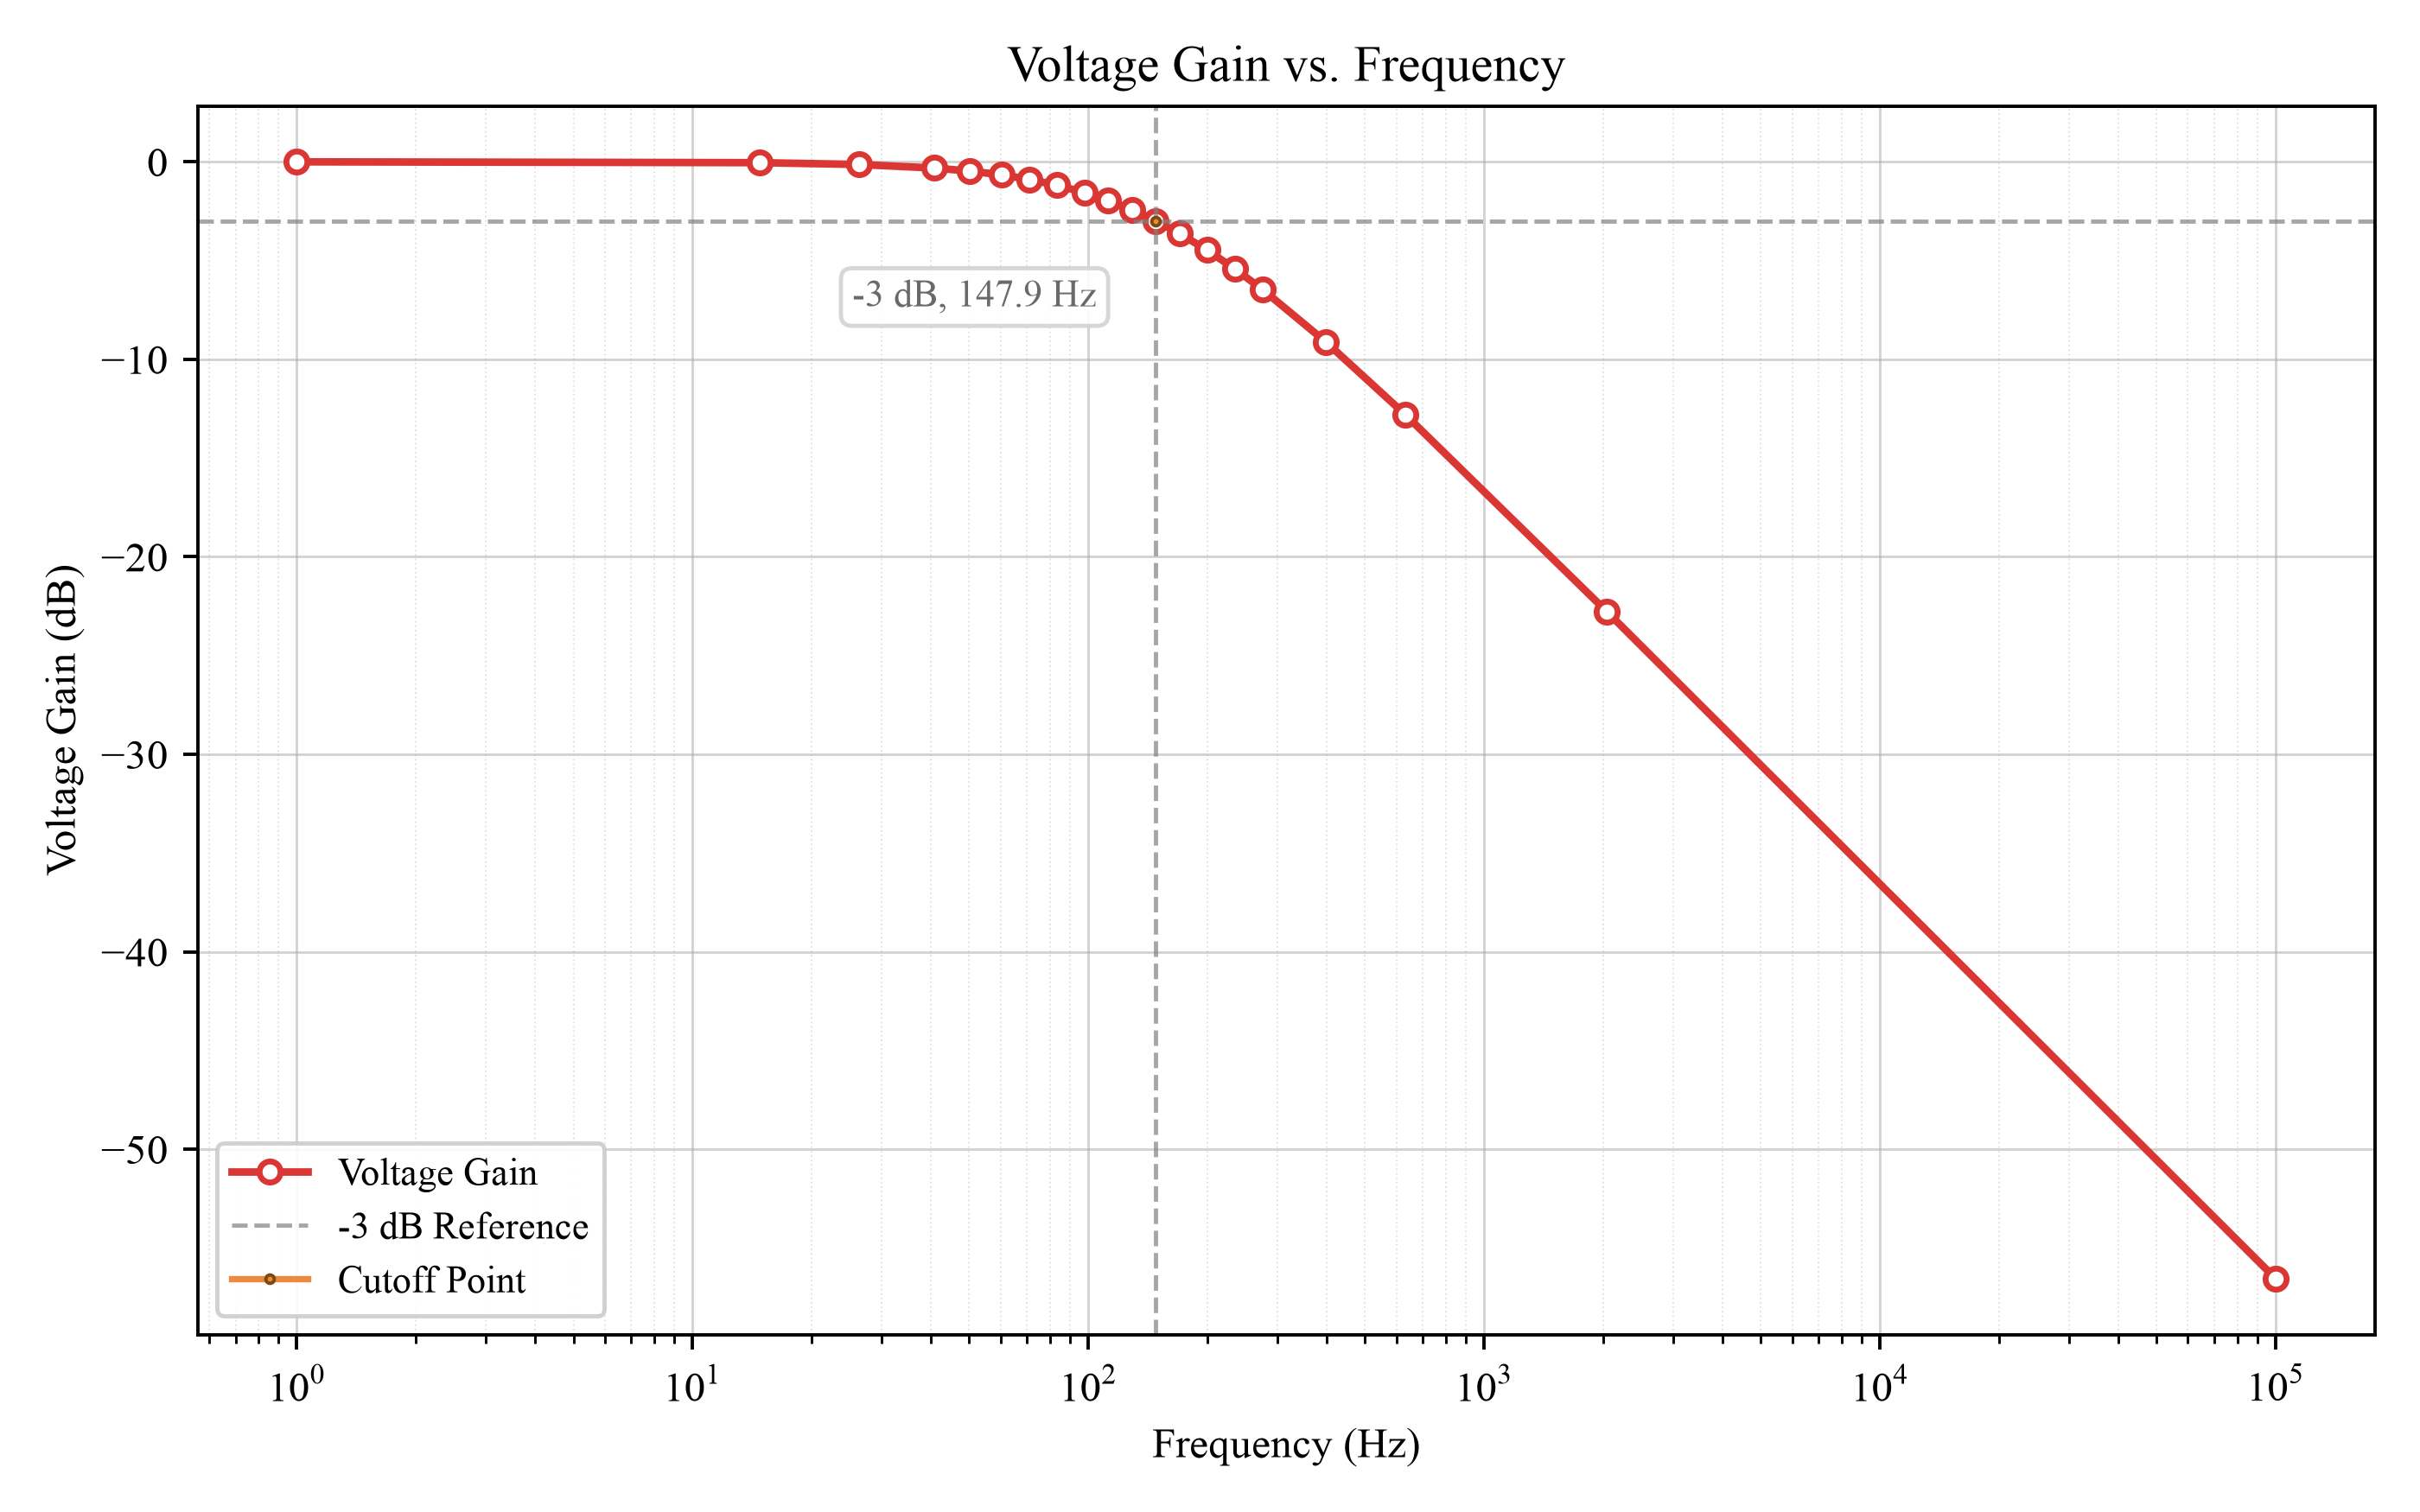
\includegraphics[width=0.85\textwidth]{OriginPro_graph_of_circuit1_gain_db_vs_freq.png}
		\caption{OriginPro gain-versus-frequency curve of the low-pass filter}
		\label{fig:og1}
	\end{figure}
	
	\begin{figure}[H]
		\centering
		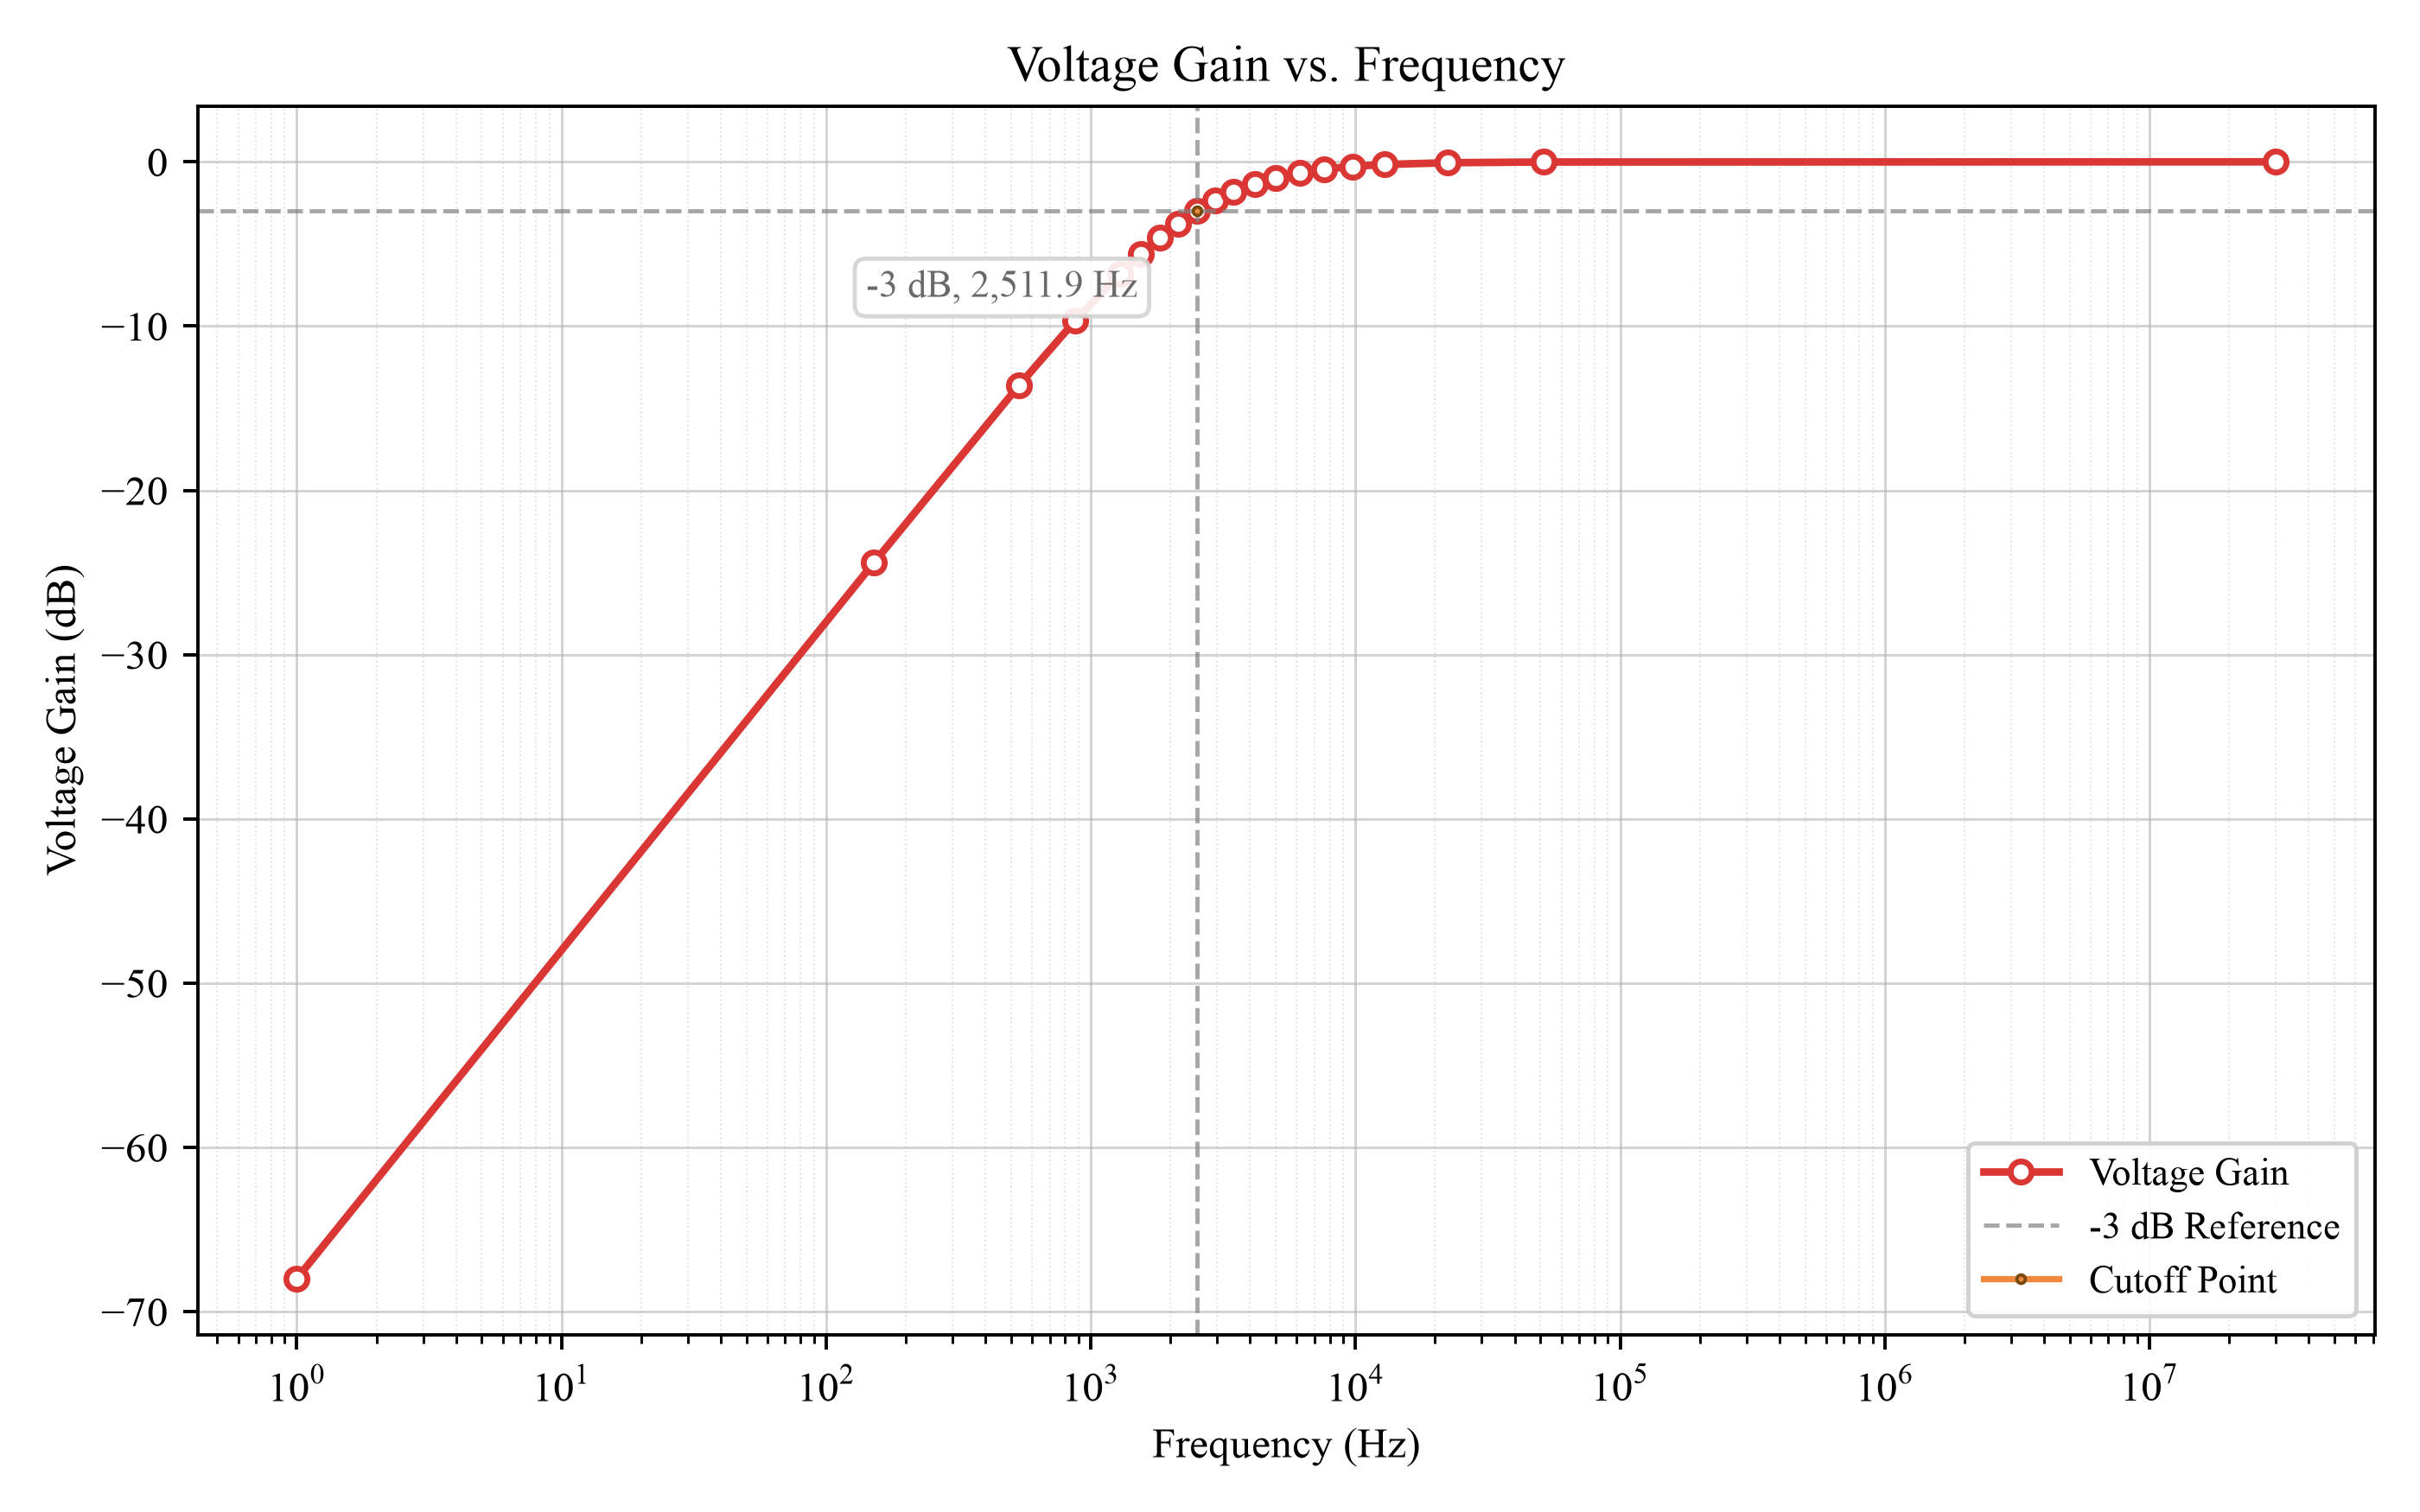
\includegraphics[width=0.85\textwidth]{OriginPro_graph_of_circuit2_gain_db_vs_freq.png}
		\caption{OriginPro gain-versus-frequency curve of the high-pass
			filter}
		\label{fig:og2}
	\end{figure}
	
	\begin{figure}[H]
		\centering
		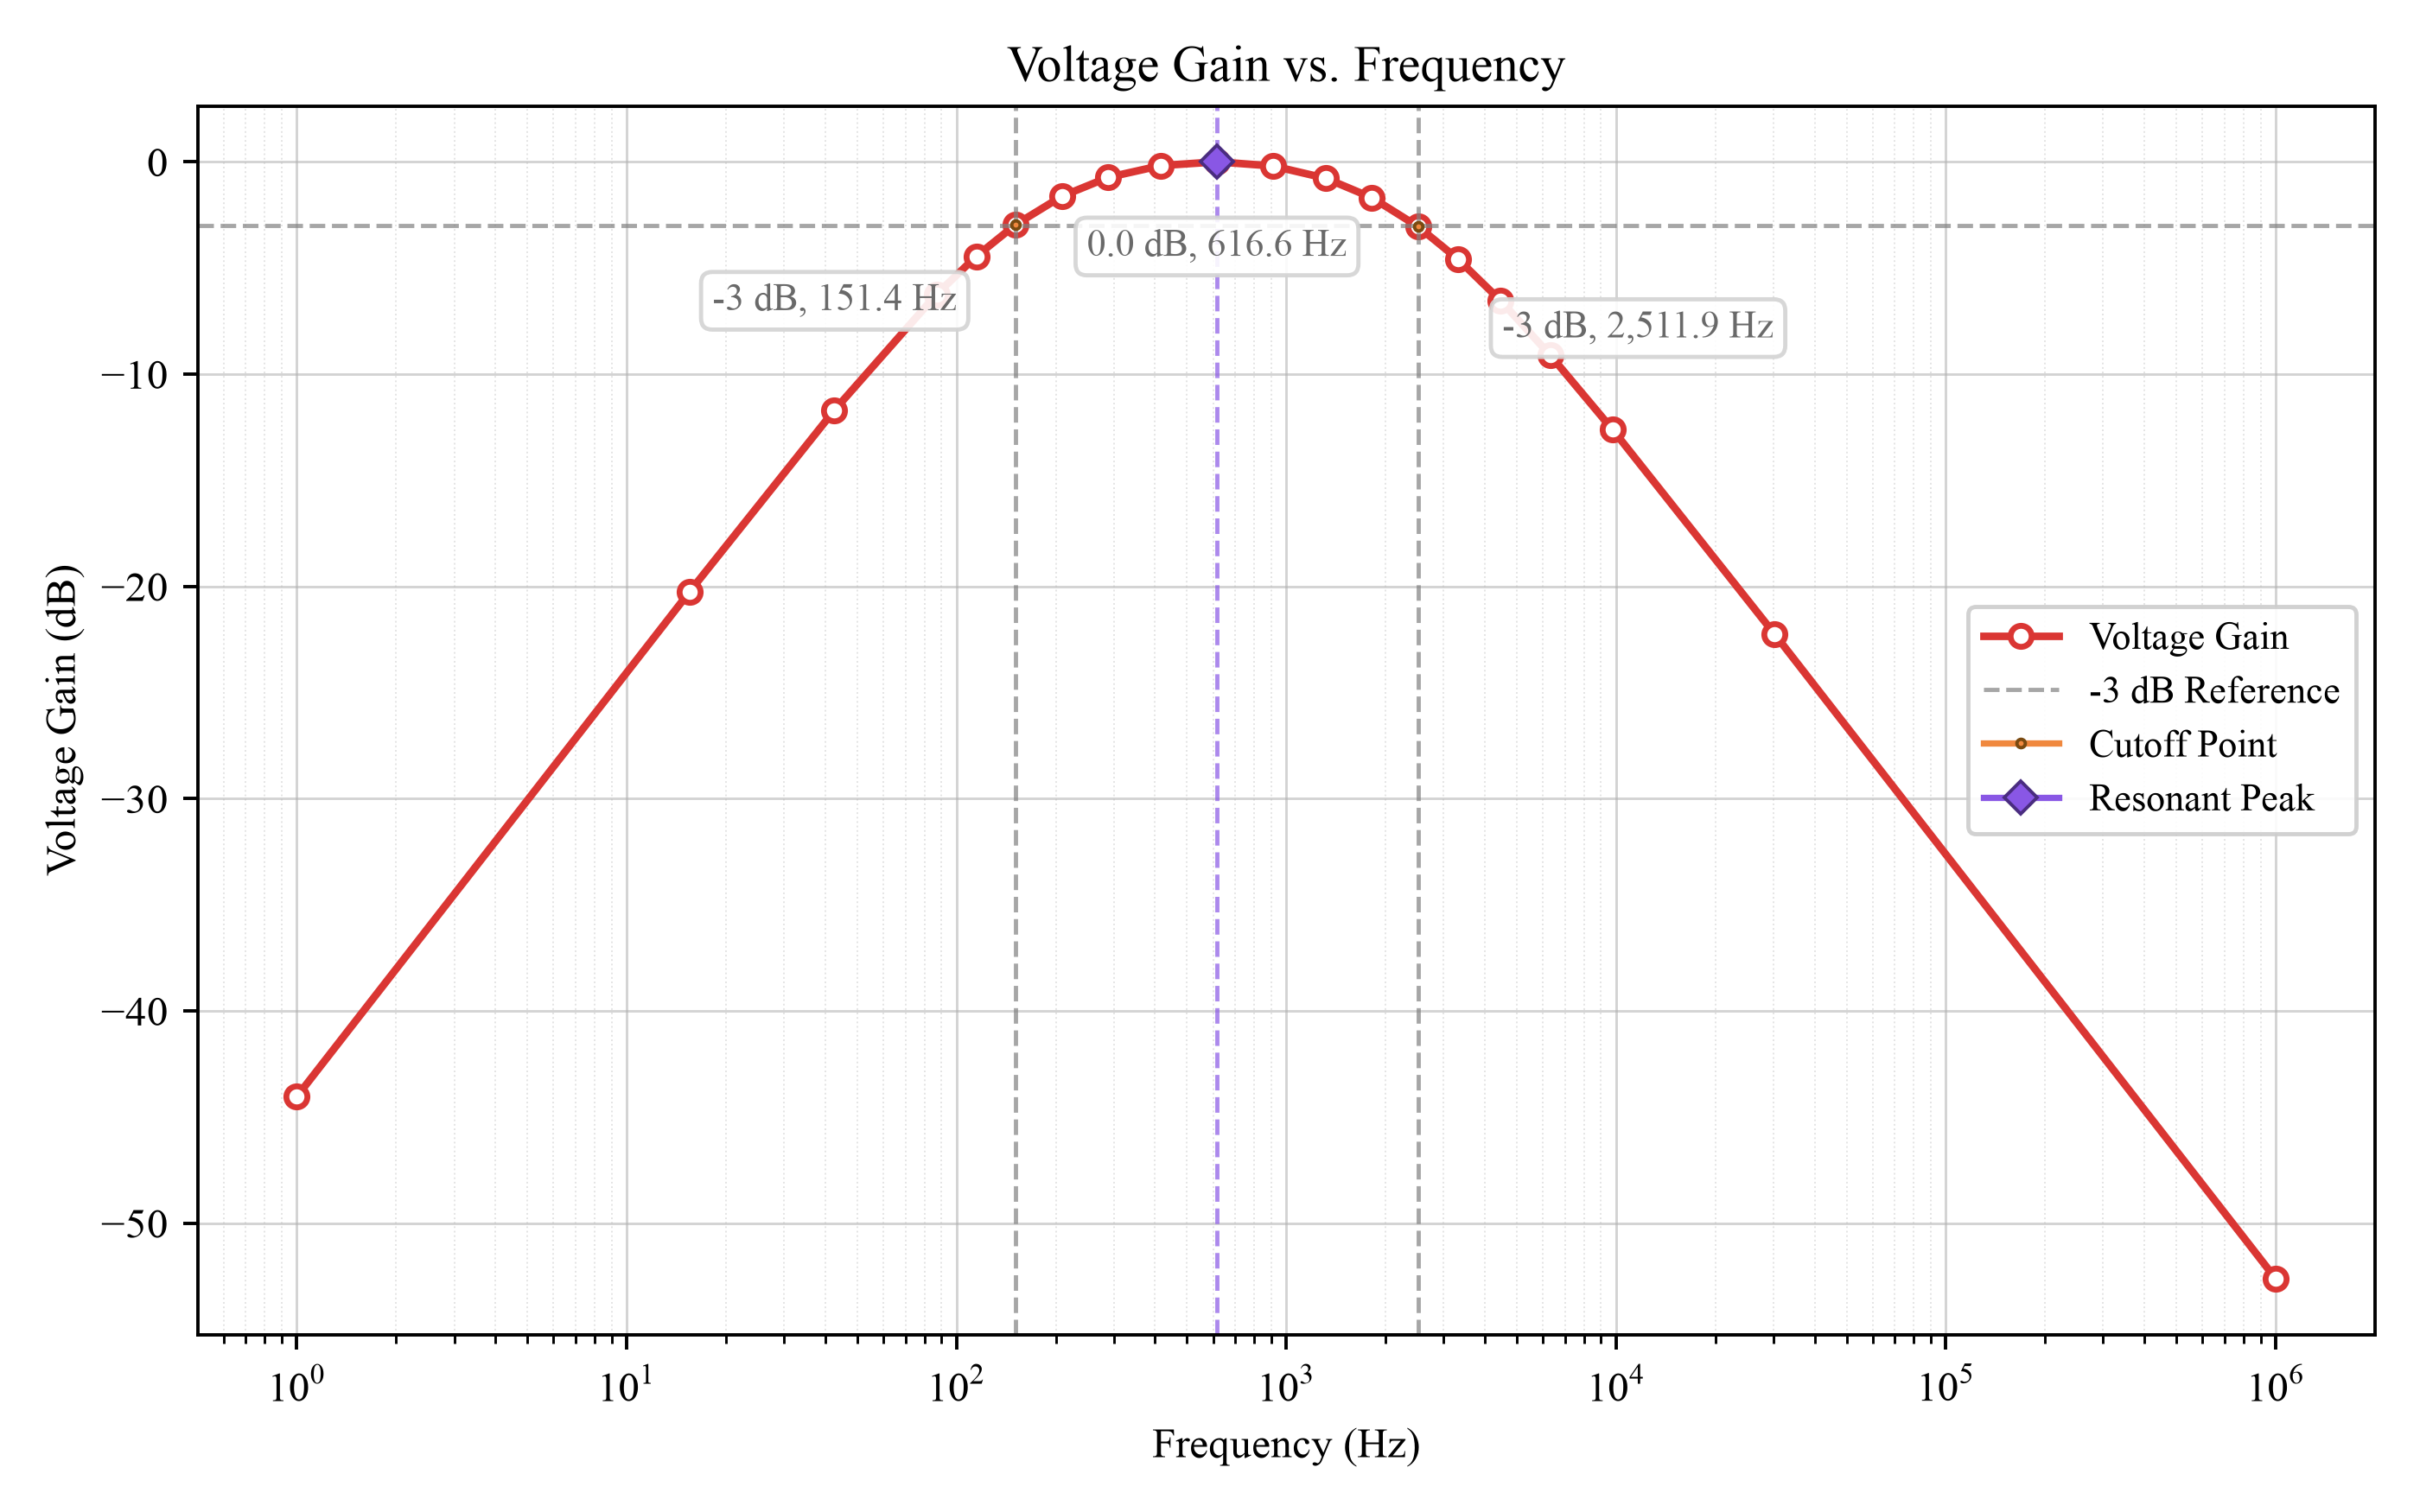
\includegraphics[width=0.85\textwidth]{OriginPro_graph_of_circuit3_gain_db_vs_freq.png}
		\caption{OriginPro gain-versus-frequency curve of the band-pass
			filter}
		\label{fig:og3}
	\end{figure}
	
	\begin{figure}[H]
		\centering
		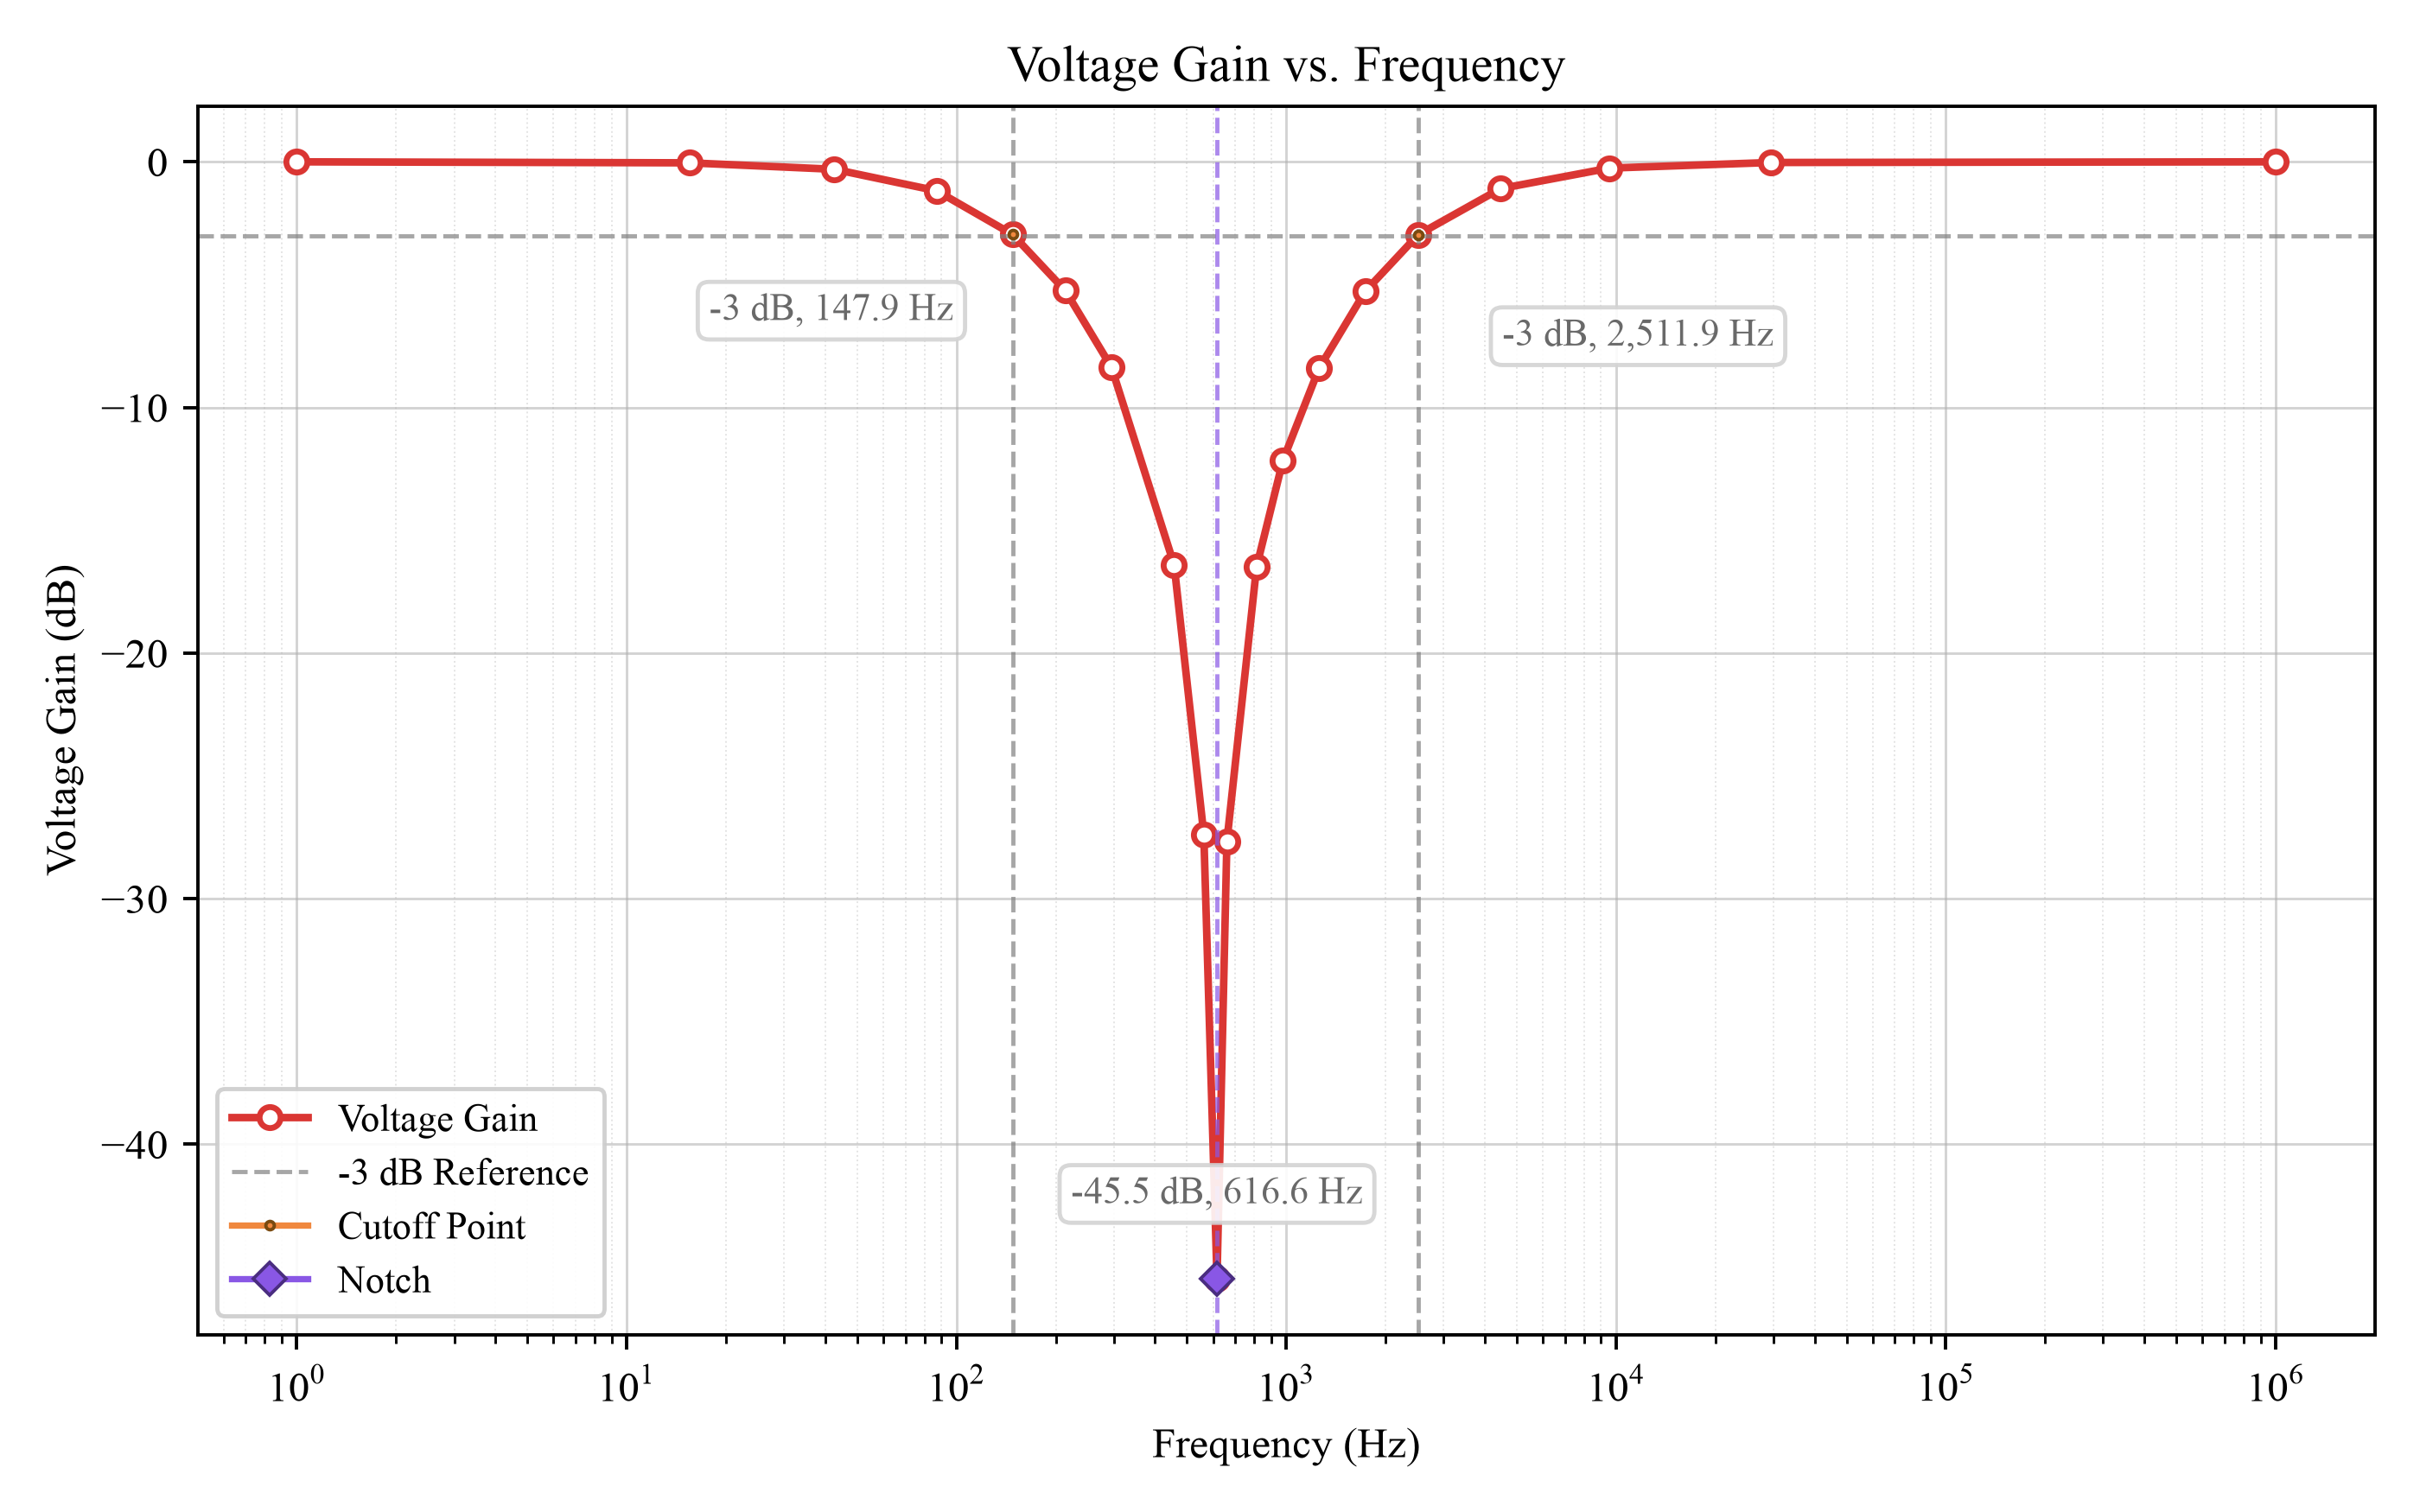
\includegraphics[width=0.85\textwidth]{OriginPro_graph_of_circuit4_gain_db_vs_freq.png}
		\caption{OriginPro gain-versus-frequency curve of the band-stop
			filter}
		\label{fig:og4}
	\end{figure}
	
	\begin{figure}[H]
		\centering
		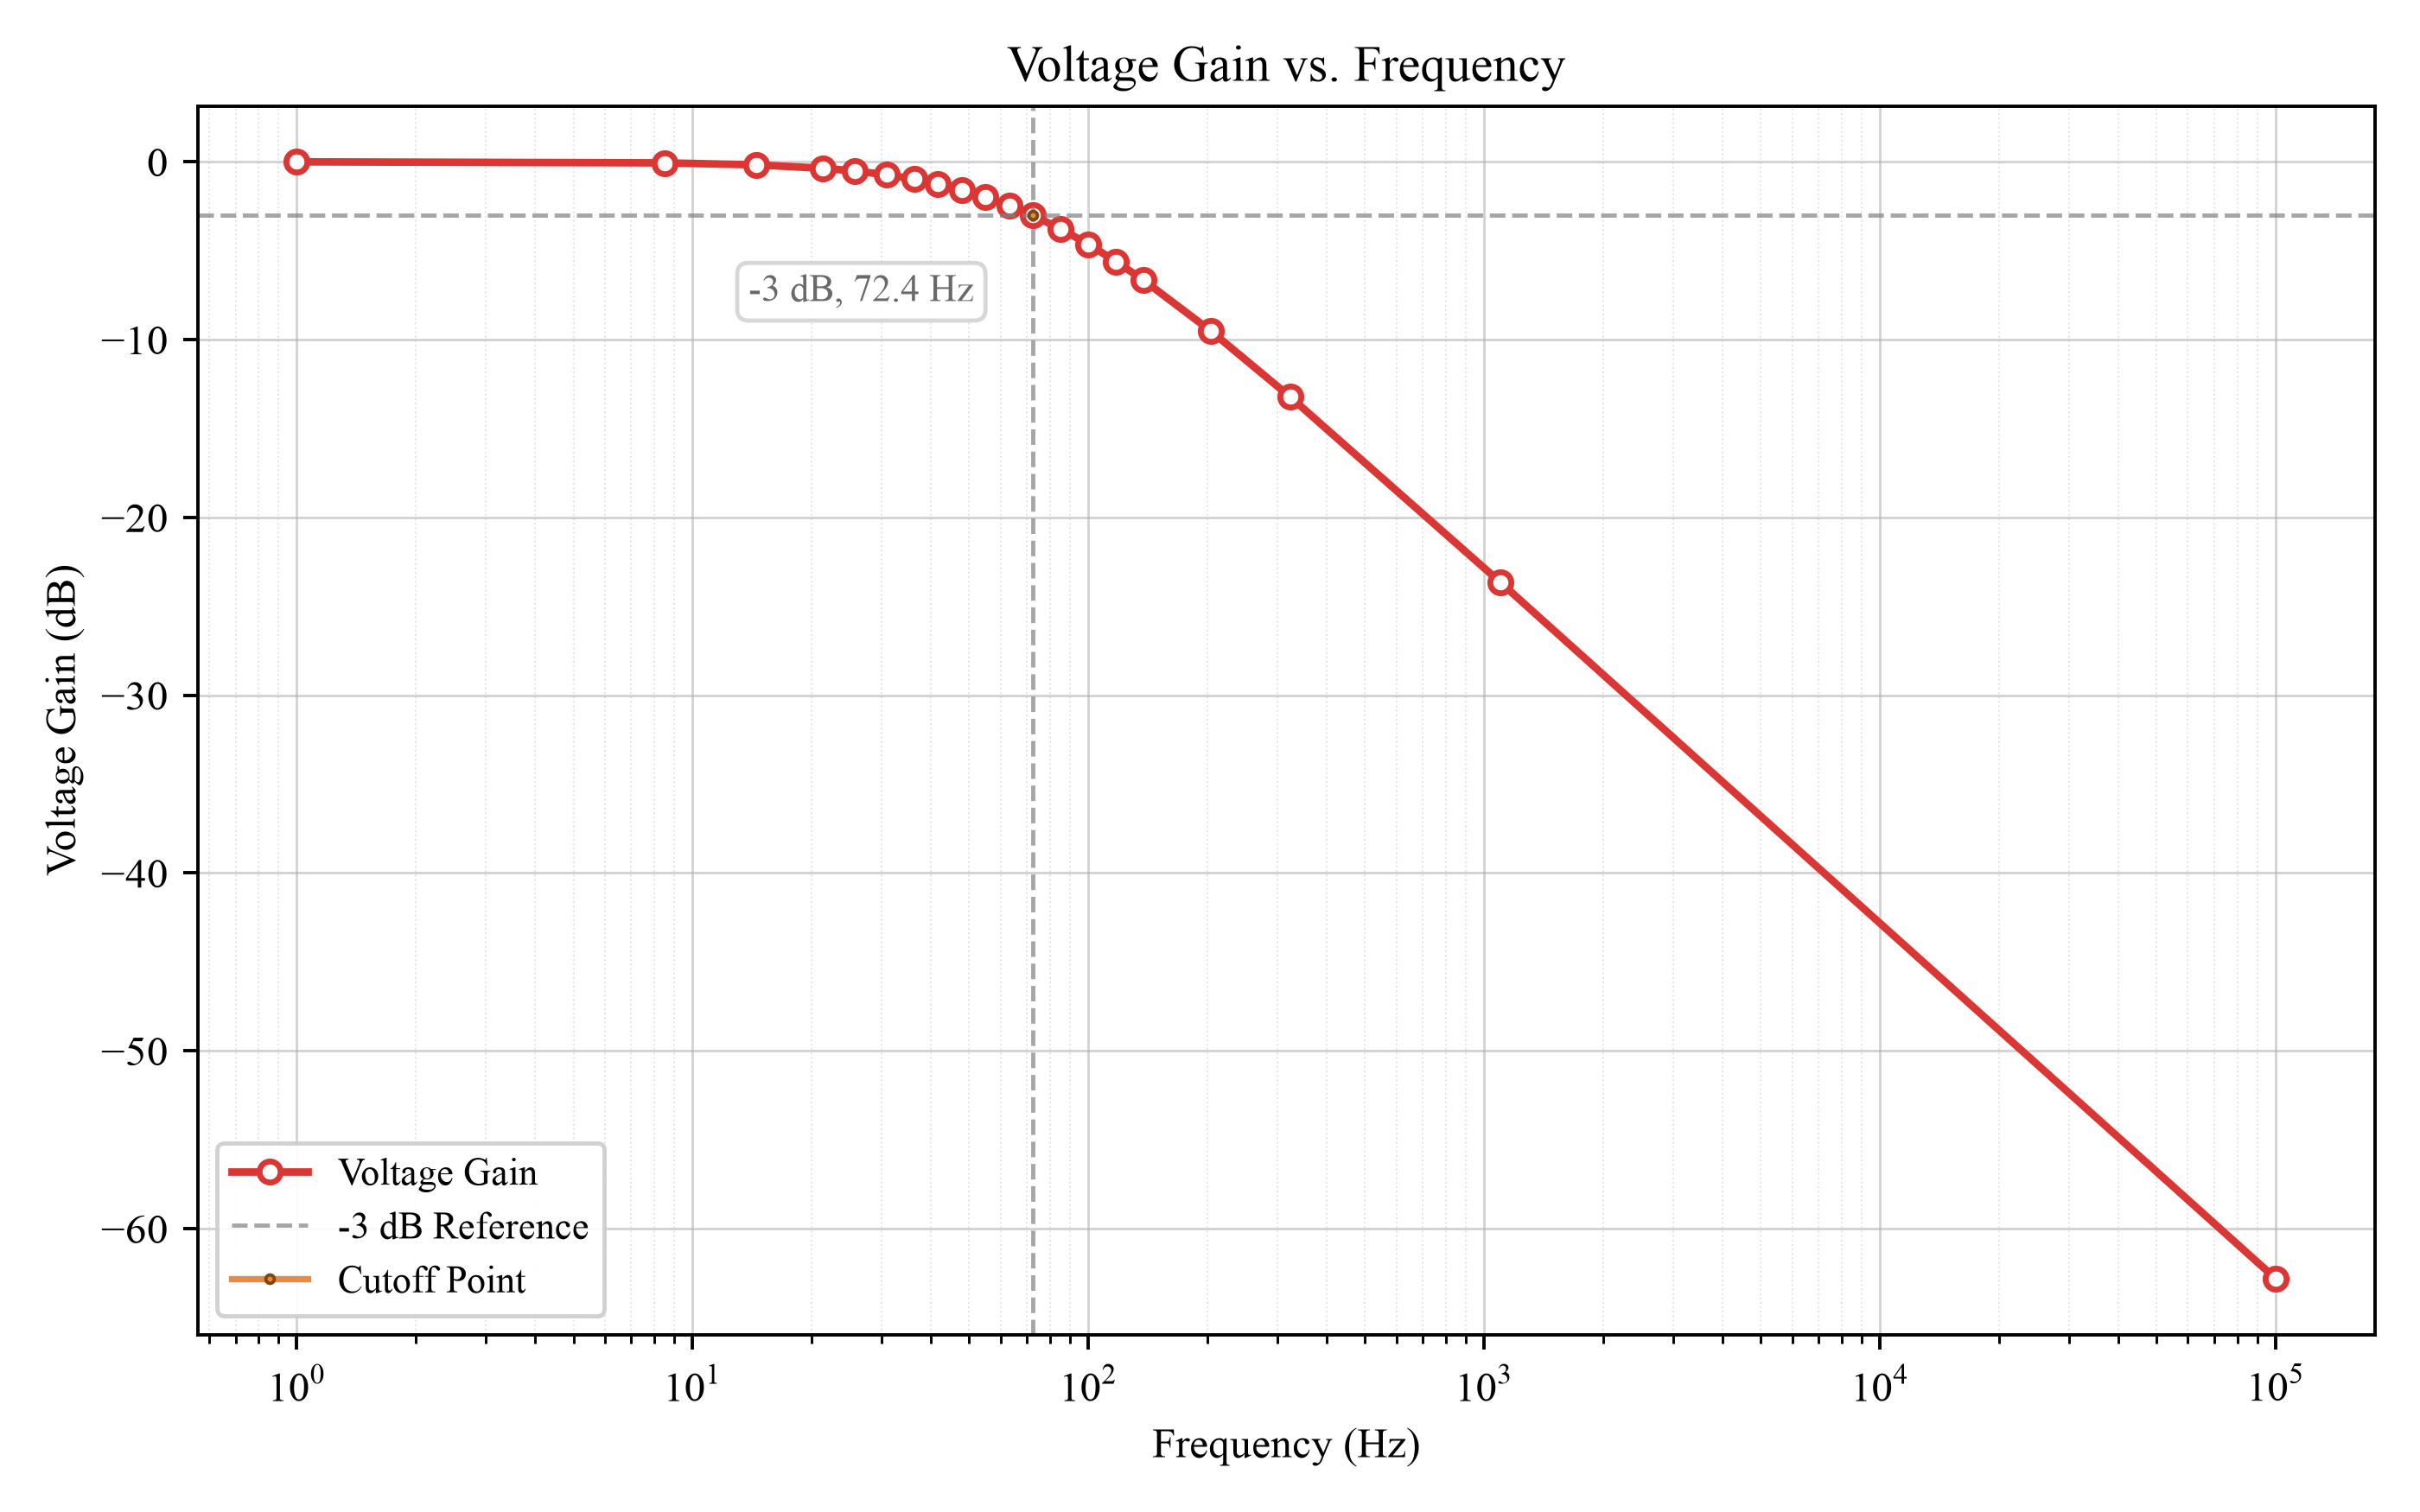
\includegraphics[width=0.85\textwidth]{OriginPro_graph_of_circuit1_changed_gain_db_vs_freq.png}
		\caption{OriginPro gain-versus-frequency curve of the modified
			low-pass filter (task 7)}
		\label{fig:ogc}
	\end{figure}
	
	\subsection{Comparison of formula, theoretical, and simulated frequencies (task 6)}
	Table~\ref{tab:compare} collects the class-roll formula targets, the
	theoretical values computed from the standard component values in
	Section 2.7, and the simulated values extracted from the data with the
	70.7\% criterion. Percentage error is defined as
	\[
	\%\ \text{error} =
	\left|\frac{\text{Theoretical} - \text{Simulated}}{\text{Theoretical}}\right| \times 100.
	\]
	
	\begin{table}[H]
		\centering
		\caption{Formula targets vs.\ theoretical vs.\ simulated characteristic
			frequencies; percentage error is theory vs.\ simulation}
		\label{tab:compare}
		\small
		\renewcommand{\arraystretch}{1.25}
		\begin{tabular}{|l|l|r|r|r|r|}
			\hline
			\rowcolor{black!12}\textbf{Circuit} & \textbf{Quantity} & \textbf{Formula} & \textbf{Theoretical} &
			\textbf{Simulated} & \textbf{\% Error} \\
			\hline
			1 (LP) & $f_c$ & 150.0 Hz & 148.7 Hz & 148.74 Hz & $0.03$ \\
			\hline
			2 (HP) & $f_c$ & 2500.0 Hz & 2510.3 Hz & 2510.35 Hz & $0.00$ \\
			\hline
			\multirow{5}{*}{3 (BP)}
			& $f_L$ & 150.0 Hz & 149.6 Hz & 149.59 Hz & $0.01$ \\
			\cline{2-6}
			& $f_H$ & 2500.0 Hz & 2490.1 Hz & 2490.05 Hz & $0.00$ \\
			\cline{2-6}
			& $f_0$ & 612.4 Hz & 610.3 Hz & 610.33 Hz & $0.00$ \\
			\cline{2-6}
			& $BW$ & 2350.0 Hz & 2340.5 Hz & 2340.5 Hz & $0.00$ \\
			\cline{2-6}
			& $Q$ & 0.2606 & 0.2608 & 0.2608 & $0.00$ \\
			\hline
			\multirow{5}{*}{4 (BS)}
			& $f_L$ & 150.0 Hz & 149.6 Hz & 149.58 Hz & $0.01$ \\
			\cline{2-6}
			& $f_H$ & 2500.0 Hz & 2490.1 Hz & 2490.3 Hz & $0.01$ \\
			\cline{2-6}
			& $f_0$ & 612.4 Hz & 610.3 Hz & 611.8 Hz & $0.25$ \\
			\cline{2-6}
			& $BW$ & 2350.0 Hz & 2340.5 Hz & 2340.7 Hz & $0.01$ \\
			\cline{2-6}
			& $Q$ & 0.2606 & 0.2608 & 0.2614 & $0.23$ \\
			\hline
			1 changed (LP) & $f_c$ & 150.0 Hz & 72.3 Hz & 72.36 Hz & $0.08$ \\
			\hline
		\end{tabular}
	\end{table}
	Every simulated quantity agrees with its theoretical value to better
	than $0.3\%$. The deviation of the theoretical values from the
	formula targets (at most $0.84\%$, e.g.\ $148.7\ \mathrm{Hz}$ against
	$150\ \mathrm{Hz}$ for the low-pass filter) is not a simulation
	discrepancy: it is the deliberate consequence of rounding the designed
	component values to standard series values (Section 2.3).
	
	\subsection{Effect of changing R and C (task 7)}
	Table~\ref{tab:task7} compares the original and modified low-pass
	filters.
	
	\begin{table}[H]
		\centering
		\caption{Low-pass filter before and after changing R and C}
		\label{tab:task7}
		\renewcommand{\arraystretch}{1.25}
		\begin{tabular}{|l|c|c|}
			\hline
			\rowcolor{black!12}\textbf{Quantity} & \textbf{Original (circuit 1)} & \textbf{Modified (task 7)} \\
			\hline
			$R$ & \SI{10.7}{\kilo\ohm} & \SI{2.2}{\kilo\ohm} \\
			\hline
			$C$ & \SI{100}{\nano\farad} & \SI{1}{\micro\farad} \\
			\hline
			$RC$ & \SI{1.07}{\milli\second} & \SI{2.2}{\milli\second} \\
			\hline
			Theoretical $f_c$ & \SI{148.7}{\hertz} & \SI{72.3}{\hertz} \\
			\hline
			Simulated $f_c$ & \SI{148.74}{\hertz} & \SI{72.36}{\hertz} \\
			\hline
			\% Error & $0.03$ & $0.08$ \\
			\hline
		\end{tabular}
	\end{table}
	
	Although the resistor was \emph{decreased} from
	\SI{10.7}{\kilo\ohm} to \SI{2.2}{\kilo\ohm}, the cutoff frequency also
	decreased by a factor of about 2.05, because the capacitor was
	increased tenfold while the resistor was only decreased by a factor of
	4.86; the product $RC$ (hence $1/2\pi RC$) governs. The overall shape
	of the response is unchanged.
	
	% =====================================================================
	\section{Discussion}
	% =====================================================================
	All four filter types behaved exactly as the derived theory predicts.
	The low-pass response is flat near unity gain and falls at
	$-20\ \mathrm{dB/decade}$ beyond $f_c$; the high-pass response is its
	mirror image; the band-pass curve peaks at $f_0 = \SI{610}{\hertz}$
	with a gain of essentially 1, and the band-stop curve shows the
	complementary deep notch at the same frequency. Since both RLC filters
	share one loop and differ only in the output terminals, their cutoff
	frequencies come from the same condition $|X(\omega)| = R$ and agree
	with each other within the interpolation tolerance.
	
	The agreement between simulation and theory (percentage errors below
	$0.3\%$, Table \ref{tab:compare}) is far better than one would obtain
	with physical components. This is expected: the PSpice models are
	ideal lumped elements at the specified values, that is there are no
	tolerances, parasitics, or meter-loading effects; and the AC solver
	evaluates the same node equations derived in Section 2.2. The
	residual sub-percent discrepancies are therefore numerical rather
	than physical: the manually tabulated data of Tables~\ref{tab:data1}--\ref{tab:datac} contain only 20 logarithmically spaced
	points, so the true $-3\ \mathrm{dB}$ crossing usually falls between
	samples and the interpolated value inherits a small error from the
	curvature of the response on the log-log grid. A denser sweep would
	reduce the residuals further.
	
	The formula/theoretical/simulated distinction deserves emphasis. The
	class-roll formula specifies an ideal target (e.g.\ \SI{150}{\hertz}),
	but only standard E-series components are available; choosing, say,
	\SI{10.7}{\kilo\ohm} instead of the exactly required
	\SI{10.61}{\kilo\ohm} shifts the true cutoff to \SI{148.7}{\hertz}.
	Grading the simulation against the formula directly would wrongly
	attribute this intentional design rounding to simulation error, which
	is why the standard-value theory is the proper reference and
	against it the simulation is essentially exact.
	
	Changing $R$ and $C$ (task 7) illustrates the inverse-proportional
	dependence $f_c \propto 1/RC$. A first-order filter's cutoff is set by
	the single time constant $RC$; only the \emph{product} matters, which
	is why very different $R$/$C$ pairs yield the same response shape and
	the frequency simply scales with $1/RC$. The unchanged
	$-20\ \mathrm{dB/decade}$ slope confirms that the filter order is a
	property of the topology (one energy-storage element), not of the
	component values. For the RLC pair, by contrast, $f_0$ depends only on
	$L$ and $C$ while the bandwidth depends on $R/L$: increasing $R$ would
	widen the band and reduce $Q$ (already low here, $Q \approx 0.26$,
	which is why the passband is very wide with gentle skirts), whereas
	increasing $L$ or $C$ would pull $f_0$ down without changing $Q$'s
	dependence on $L/C$ alone ($Q \propto \sqrt{L/C}$).
	
	Two waveform details are worth noting. The circuit-4 notch bottoms out
	near $-45.5\ \mathrm{dB}$ in the read data, but the theoretical null is
	complete ($|H_{\mathrm{BS}}|\to 0$ at $f_0$ because the series $LC$
	branch becomes a short); the finite floor is again a sweep-sampling
	artefact, the nearest sample point does not fall exactly on $f_0$.
	Likewise, the high-pass gain at \SI{1}{\hertz} ($\approx -68\ \mathrm{dB}$)
	matches the predicted asymptote $20\log_{10}(f/f_c)$. Practically,
	the experiment shows that passive filters are simple, robust and
	require no power supply, but their selectivity is limited by the
	low $Q$ achievable with passive elements: for narrow bands one needs
	high-$Q$ coils or active topologies, since loading by the source and
	measuring instrument (idealised away here) further degrades real
	passive responses.
	
	% =====================================================================
	\section{Reference}
	% =====================================================================
	\renewcommand{\refname}{} % suppress duplicate heading; \section{Reference} above serves
	\begin{thebibliography}{9}
		\bibitem{ref:sadiku} C. K. Alexander and M. N. O. Sadiku,
		\textit{Fundamentals of Electric Circuits}, 5th ed. New York,
		NY, USA: McGraw-Hill, 2013, ch.~14, sec.~14.3--14.7,
		pp.~617--641.
		\bibitem{ref:boylestad} R. L. Boylestad, \textit{Introductory
			Circuit Analysis}, 13th ed. Harlow, U.K.: Pearson Education,
		2016, chs.~21 and 22, pp.~921--1046.
	\end{thebibliography}
	
\end{document}